\documentclass[a4paper]{article}
%\documentclass[aps,prd,preprint,nofootinbib]{revtex4-1}
\pdfoutput=1
\linespread{1}
\usepackage[T1]{fontenc}
\usepackage{amssymb}
\usepackage{url}
\usepackage{graphicx}
\usepackage{xspace}
\usepackage[svgnames]{xcolor}
\usepackage[caption=false]{subfig}
\usepackage{setspace}
\usepackage{amsmath}
\usepackage{listings} 
\usepackage[normalem]{ulem}
\usepackage{placeins}
%\usepackage{braket}
\usepackage{multirow}
\usepackage{tabulary}
\usepackage{hyperref}% add hypertext capabilities
\usepackage{dcolumn}% Align table columns on decimal point
\usepackage{bm}% bold math
\usepackage{soul}
%\usepackage{makecell}

\usepackage[utf8]{inputenc} % utf8 support in source code
\usepackage[a4paper,top=3cm,bottom=2cm,left=3cm,right=3cm,marginparwidth=1.75cm]{geometry}

\usepackage[autostyle]{csquotes} % recommended by biblatex
\usepackage{xpatch} % recommended by biblatex
\usepackage[backend=biber, giveninits, sorting=none, style=numeric-comp]{biblatex} % much more flexible than BibTeX
\addbibresource{bibliography.bib}

\usepackage{siunitx}
\sisetup{separate-uncertainty=true}

\newcommand{\todo}[1]{{\color{red} (To Do: #1)}}
\newcommand{\blue}[1]{\textcolor{NALblue}{#1}}
\newcommand\addcite{[{\color{blue} \underline{CITATION NEEDED}}]}

\newcommand{\enu}{\ensuremath{E_{\nu}}\xspace}
\def\bracketbar{\hbox{\kern-9pt\raise1pt%
    \hbox{{\tiny(}{\lower1.5pt\hbox{\bf--}}{\tiny)}}}}

\begin{document}


\begin{center}
		
	{\Large \bf ProtoDUNE-ND: proposal to place the ArgonCube 2x2 Demonstrator module in a neutrino beamline at Fermilab} 
	\vspace*{0.5cm}
	\setcounter{footnote}{0}  
	\def\A{\kern+.6ex\lower.42ex\hbox{$\scriptstyle \iota$}\kern-1.20ex a}
	\def\E{\kern+.5ex\lower.42ex\hbox{$\scriptstyle \iota$}\kern-1.10ex e}
	\small
	\newcommand{\Aname}[2]{#1}
	\def\titlefoot#1{\vspace{-0.3cm}\begin{center}{\bf #1}\end{center}}
	
	\Aname{M.~Auger}{Bern},
	\Aname{R.~Berner}{Bern},
	\Aname{Y.~Chen}{Bern},
	\Aname{A.~Ereditato}{Bern},
	\Aname{D.~Goeldi\footnote{Now at Department of Physics, Carleton University, Ottawa, Ontario, K1S 5B6, Canada}}{Bern},
	\Aname{P.~P.~Koller}{Bern},
	\Aname{I.~Kreslo}{Bern},
	\Aname{D.~Lorca}{Bern},
	\Aname{T.~Mettler}{Bern},
	\Aname{F.~Piastra}{Bern},
	\Aname{J.~R.~Sinclair\footnote{Corresponding author: james.sinclair@lhep.unibe.ch}}{Bern},
	\Aname{M.~Weber}{Bern} and
	\Aname{C.~Wilkinson\footnote{Corresponding author: callum.wilkinson@lhep.unibe.ch}}{Bern}
	\titlefoot{Albert Einstein Center for Fundamental Physics (AEC), Laboratory for High Energy Physics, University of Bern, 3012 Bern, Switzerland\label{Bern}}
	
	\Aname{M.~Bishai}{BNL},
	\Aname{H.~Chen}{BNL},
	\Aname{M.~Diwan}{BNL},
	\Aname{F.~Lanni}{BNL},
	\Aname{Y.~Li}{BNL},
	\Aname{D.~Lissauer}{BNL},
	\Aname{X.~Qian}{BNL},
	\Aname{V.~Radeka}{BNL} and
	\Aname{B.~Yu}{BNL}
	\titlefoot{Brookhaven National Laboratory (BNL), Upton, NY 11973-5000, USA\label{BNL}}
	
	\Aname{M.~Mooney}{Colorado}
	\titlefoot{Colorado State University, Fort Collins, CO 80523, USA\label{colorado}}
	
	\Aname{A.~Bross}{FNAL},
	\Aname{L.~Fields}{FNAL},
	\Aname{D.~A.~Harris}{FNAL},
	\Aname{A.~Marchionni}{FNAL},
	\Aname{T.~Miao}{FNAL},
	\Aname{J.~L.~Raaf}{FNAL} and
	\Aname{J.~Zennamo}{FNAL}
	\titlefoot{Fermi National Accelerator Laboratory (FNAL), Batavia, IL 60510 USA\label{FNAL}}
	
	\Aname{R.~Guenette}{Harvard}, and
	\Aname{J.~Martin-Albo}{Harvard}
	\titlefoot{Harvard University, Cambridge, MA 02138, USA\label{Harvard}}
	
	\Aname{C.~Azevedo}{I3N},
	\Aname{A.~L.~Silva}{I3N} and
	\Aname{J.~Veloso}{I3N}
	\titlefoot{I3N, Physics Department, University of Aveiro, 3810-193 Aveiro, Portugal\label{I3N}}
	
	\Aname{N.~Anfimov}{dubna},
	\Aname{A.~Olshevskiy}{dubna},
	\Aname{A.~Selyunin}{dubna},
	\Aname{S.~Sokolov}{dubna} and
	\Aname{A.~Sotnikov}{dubna}
	\titlefoot{Joint Institute for Nuclear Research~(JINR), Joliot-Curie 6, 141980 Dubna, Moscow region, Russia\label{dubna}}
	
	\Aname{D.~Douglas}{MSU} and
	\Aname{K.~Mahn}{MSU}
	\titlefoot{Michigan State University, Department of Physics and Astronomy, East Lansing,  MI 48824, U.S.A\label{MSU}}
	
	\Aname{M.~Zeyrek}{METU}
	\titlefoot{Middle East Technical University (METU), TR-06800, Ankara, Turkey\label{METU}}
	
	\Aname{M.~Convery}{SLAC},
	\Aname{L.~Domine}{SLAC},
	\Aname{R.~Itay}{SLAC},
	\Aname{K.~Skarpaas}{SLAC},
	\Aname{H.~Tanaka}{SLAC},
	\Aname{K.~Terao}{SLAC},
	\Aname{Y-T.~Tsai}{SLAC} and
	\Aname{T.~Usher}{SLAC}
	\titlefoot{SLAC National Accelerator Laboratory and Stanford University, 2575 Sand Hill Rd, Menlo Park, CA 94025, USA\label{SLAC}}
	
	\Aname{C.~K.~Jung}{Stony},
	\Aname{C.~Vilela}{Stony},
	\Aname{M.~Wilking}{Stony} and
	\Aname{K.~Wood}{Stony}
	\titlefoot{Stony Brook University, Stony Brook, NY 11794, USA\label{Stony}}
	
	\Aname{M.~Soderberg}{Syracuse}
	\titlefoot{Syracuse University, Syracuse, NY 13210, USA\label{Syracuse}}
	
	\Aname{D.~A.~Dwyer}{LBNL},
	\Aname{D.~Gnani}{LBNL},
	\Aname{C.~Grace}{LBNL},
	\Aname{S.~Kohn}{LBNL},
	\Aname{M.~Kramer}{LBNL},
	\Aname{A.~Krieger}{LBNL},
	\Aname{K.~B.~Luk}{LBNL},
	\Aname{P.~Madigan}{LBNL} and
	\Aname{C.~Marshall}{LBNL}
	\titlefoot{University of California and Lawrence Berkeley National Laboratory, Berkeley, CA 94720, USA\label{LBNL}}
	
	\Aname{B.~Bilki}{Iowa},
	\Aname{K.~Cankocak}{Iowa},
	\Aname{J.~Nachtman}{Iowa},
	\Aname{Y.~Onel}{Iowa} and
	\Aname{A.~Penzo}{Iowa}
	\titlefoot{University of Iowa High Energy Physics Group, Iowa City, IA 52242, USA\label{Iowa}}
	
	\Aname{J.~Chaves}{UPenn} and
	\Aname{C.~M.~Mauger}{UPenn}
	\titlefoot{University of Pennsylvania,Philadelphia, PA 19104, USA\label{UPenn}}
	
	\Aname{S.~Manly}{Rochester},
	\Aname{K.~S.~McFarland}{Rochester} and
	\Aname{D.~Ruterbories}{Rocester}
	\titlefoot{University of Rochester, Rochester, NY 14627 USA\label{Rochester}}
			
	\Aname{D.~Barker}{Sheffield},
	\Aname{A.~C.~Ezeribe}{Sheffield},
	\Aname{T.~Gamble}{Sheffield},
	\Aname{N.~McConkey}{Sheffield},
	\Aname{N.~J.~C.~Spooner}{Sheffield},
	\Aname{M.~Thiesse}{Sheffield}, 
	\Aname{E.~Tyley}{Sheffield} and
	\Aname{M.~H.~Wright}{Sheffield}
	\titlefoot{University of Sheffield, Western Bank, Sheffield S10 2TN, UK\label{sheffield}}

        \newpage
	
	\Aname{C.~Kuruppu}{SC}, 
	\Aname{S.~R.~Mishra}{SC} and
	\Aname{R.~Petti}{SC}
	\titlefoot{University of South Carolina, 712 Main Street, Columbia, SC 29208 USA\label{SC}}

	\Aname{J.~Asaadi}{Arlington} and 
	\Aname{H.~Sullivan}{Arlington}
	\titlefoot{University of Texas at Arlington, Arlington, TX 76019, USA\label{Arlington}}
	
	\Aname{B.~Fleming}{YALE} and
	\Aname{S.~Tufanli}{YALE}
	\titlefoot{Yale University, Wright Laboratory, New Haven, CT 06520 USA\label{YALE}}
	
\end{center}
\vspace*{1cm}

\begin{abstract}

This document outlines the case for a neutrino beam test of the DUNE near detector (ND) at Fermilab, dubbed ProtoDUNE-ND. The proposed location for ProtoDUNE-ND is in the MINOS-ND hall, upstream of the current MINERvA/MINOS-ND locations, placing it on-axis in the NuMI medium energy neutrino beam. The core of ProtoDUNE-ND is the ArgonCube 2x2 Demonstrator module, a large scale demonstrator for the core liquid argon (LAr) component of the ND. A description of the ArgonCube 2x2 Demonstrator is given, together with a brief outline of the required infrastructure. Additionally, the possibility to include test modules for other DUNE ND component detectors is discussed. 
An overview of the detector physics studies which can be completed with ProtoDUNE-ND is given, which will inform the final DUNE ND design choices, and aid in developing reconstruction tools in preparation for DUNE.
Placing the 2x2 Demonstrator as a stand-alone underground in the NuMI beam will allow for the development and demonstration of the tools necessary to disentangle piled up events within the LAr.
In the absence of DUNE ND demonstrators for the other technologies, existing detectors can be utilised.
Pairing the 2x2 with MINERvA enables a test of the ability to track muons and fast neutrons from the slow and busy LAr detector into a fast-response detector, the keystone of the DUNE ND. 
Additionally, by pairing the 2x2 with both MINERvA and MINOS the response of 2x2 can be characterised as a function of momentum, providing a validation of the momentum measurement via multiple coulomb scattering that will need to be used for side-exiting muons in both the DUNE ND and far detector.
  
\end{abstract}



% For now suppress the table of contents
%\tableofcontents

\section{Introduction}
\label{sec:introduction}

DUNE is a next-generation accelerator neutrino oscillation experiment~\cite{DUNE, DUNE2}. DUNE will utilize an intense beam of predominantly muon (anti)neutrinos produced at Fermilab, will sample the unoscillated beam on the Fermilab site, \SI{574}{\metre} from the proton target and \SI{62}{\metre} underground, and then will sample the oscillated beam \SI{1300}{\kilo\metre} away and \SI{1.5}{\kilo\metre} underground, at the Sanford Underground Research Facility (SURF) in South Dakota, using four \SI{10}{\kilo\tonne} liquid argon (LAr) target modules. By using LAr time projection chambers (TPCs), DUNE benefits from the exquisite precision to look at the particles escaping the nucleus, and measuring the neutrino energies with unparalleled accuracy. An extensive research and development (R\&D) program is currently ongoing to deliver detectors capable of fulfilling DUNE's physics goals. The unprecedented size of the DUNE far detectors~\cite{DUNE_IDR_v1, DUNE_IDR_v2, DUNE_IDR_v3} has motivated large-scale LAr TPC tests, in the single- and dual-phase ProtoDUNE modules in CERN~\cite{Abi:2017aow, Agostino:2014qoa}, in themselves, the largest LAr TPCs built to date.

As the DUNE far detectors have LAr targets, there will also be a major LAr component for the DUNE near detector suite, in order to minimize cross section and detector systematic uncertainties for oscillation analyses~\cite{DUNE, DUNE2}. However, the intense neutrino flux and high event rate at the near detector makes traditional, monolithic, projective wire readout TPCs unsuitable, which has motivated a program of R\&D into a new LAr TPC approach, suitable for such a high rate environment, known as ArgonCube~\cite{argoncube_loi}. ArgonCube utilizes detector modularization to improve drift field stability, reducing high voltage (HV) and the LAr purity requirements; it uses a pixelized charge readout~\cite{pixels, larpix}, which provides unambiguous 3D imaging of particle interactions drastically simplifying the reconstruction; and new dielectric light detection techniques with ArCLight~\cite{arclight}, which can be placed inside the field cage to increase light yield, and localization of light signals. Additionally, ArgonCube uses a resistive field shell, instead of traditional field shaping rings, to minimize the dead material and maximize active volume, and to minimize the power release in the event of a breakdown~\cite{argoncube_fd}. Such an optically segmented, pixel readout LAr TPC has been recommended as the major LAr component for the DUNE near detector by the DUNE Near Detector Concept Study Group~\cite{dune_ndcsg}.

Early investigations in Bern into long drift lengths and high electric fields with the ArgonTube detector~\cite{argontube_design} found a number of technical issues and a higher than expected risk of breakdowns~\cite{argontube}, as well as testing cryogenic charge readout electronics~\cite{art_cold_ero}. Smaller, modular, LAr TPCs were introduced as a robust solution to the high voltage problem, which reduces the LAr purity requirements due to the short drift lengths, and which have obvious advantages in high multiplicity environments. The feasibility of pixelated readout was demonstrated using a 60-cm-drift pixel TPC located at the University of Bern in 2016~\cite{pixels}. LArIAT~\cite{lariat} has since operated a scaled-up version of this readout technique (renamed PixLAr) at Fermilab in 2017. The recent development of the LArPix pixel readout electronics by LBNL have removed the ambiguities present for the earlier tests~\cite{larpix}. The 60-cm-drift pixel TPC, and a 10-cm version at LBNL, were used to demonstrate cold amplification and cold digitization with the first version of the LArPix electronics~\cite{larpix}. A field-shell demonstrator TPC was tested successfully in Bern in 2018~\cite{argoncube_fd}. Tests of the ArCLight dielectric photon detector have also been carried out in LAr, as described in Ref.~\cite{arclight}. With the various technological developments demonstrated with small-scale TPCs, the next necessary step in the ArgonCube program is to demonstrate the scalability of the pixelized charge readout and light detection systems, and to show that information from separate modules can be combined to produce high quality event reconstruction for particle interactions. To that end, a mid-scale (\SI[product-units=repeat]{1.4x1.4x1.2}{\metre}) modular TPC, dubbed the ArgonCube 2x2 Demonstrator, with 4 independent LAr TPC modules arranged in a 2x2 grid has been designed, and is currently under construction in Bern. Given the environment that the DUNE near detector will operate in, it is desirable to operate the ArgonCube 2x2 Demonstrator in an intense, few-GeV, neutrino beam.


In this document, we propose moving the ArgonCube 2x2 Demonstrator into the NuMI on-axis neutrino beamline at FNAL, to serve as the core of a prototype for the near detector, or ProtoDUNE-ND. This is in analogy to the successful ProtoDUNE program for the far detector. A detailed description of the proposed location and the ArgonCube 2x2 Demonstrator module can be found in Section~\ref{sec:protodune-nd}. A description of the detector physics studies to be performed with the 2x2 alone is given in Section~\ref{sec:detector-physics-studies}. Additional detector physics possibilities if a downstream tracker is added to ProtoDUNE-ND are described in Section~\ref{sec:MINERvA_MINOS}, with the option of repurposing existing MINERVA and/or MINOS ND hardware is discussed. The outlook for the test modules and a timeline in Section~\ref{sec:outlook}. Conclusions are presented in Section~\ref{sec:conclusions}.


\section{ProtoDUNE-ND}
\label{sec:protodune-nd}
In this section, the technical design of the proposed ProtoDUNE-ND at Fermilab is described. First, a consideration of the available neutrino beamlines at Fermilab is carried out in Section~\ref{sec:neutrino-flux}, which shows that the on-axis medium-energy NuMI beam provides a rate closest to that of the future, intense, LBNF beamline~\cite{DUNE3, dune_opt_flux}, making the MINOS hall the ideal location for this prototype. Second, a discussion of the MINOS near detector hall is provided in Section~\ref{sec:minos-hall}, with consideration given to the existing and required infrastructure to support the ProtoDUNE-ND detectors. Then, a discussion of the technical aspects of the ProtoDUNE-ND detector design is given: a description of the ArgonCube 2x2 Demonstrator module is given in Section~\ref{sec:2x2-design}, and a description of potential downstream tracking detectors is given in Section~\ref{sec:tracking_detectors}. %\todo{Modify as appropriate... if there's only ArgonCube information available, we can note the possibility of others being included, and comment on the branch points when decisions about whether to include them or not must be made.}

\subsection{Neutrino flux study}
\label{sec:neutrino-flux}
The LBNF beamline is an intense source of muon (anti-)neutrinos, with a much higher flux of neutrinos than accelerator neutrino beams currently in operation~\cite{DUNE3,dune_opt_flux}. A key design requirement for the DUNE near detectors, and one of the primary concerns motivating this ProtoDUNE-ND proposal, is how well the near detector components will perform in a high multiplicity environment. It is therefore worth asking how suitable existing beamlines are for providing a useful neutrino beam test for the proposed near detector components.

\begin{figure}[htb]
  \centering
  \subfloat[Flux\label{subfig:flux}]    {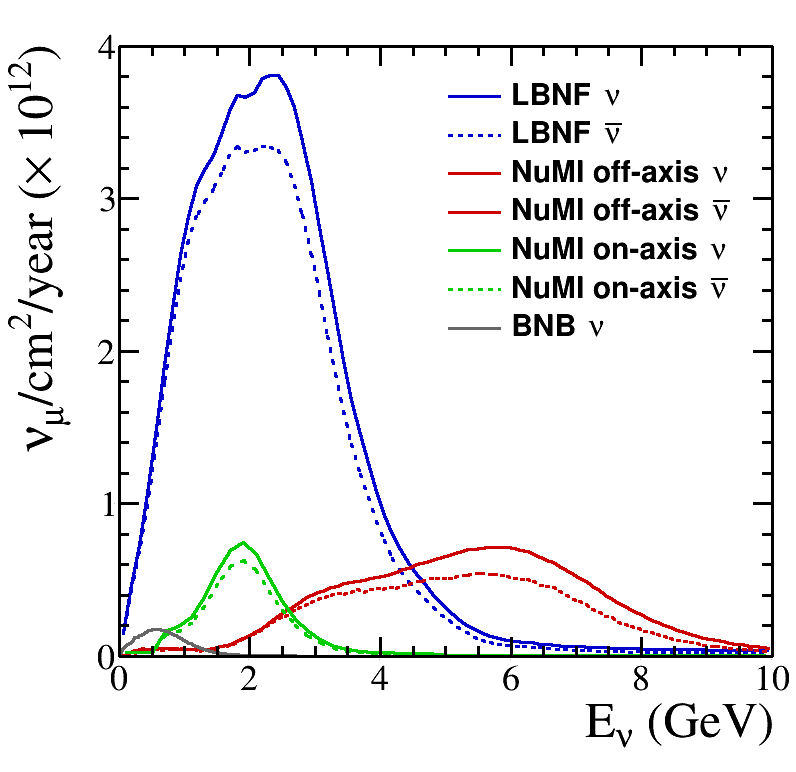
\includegraphics[width=0.5\textwidth]{plots/fnal_flux_comparison.png}}
  \subfloat[Rate\label{subfig:rate}]    {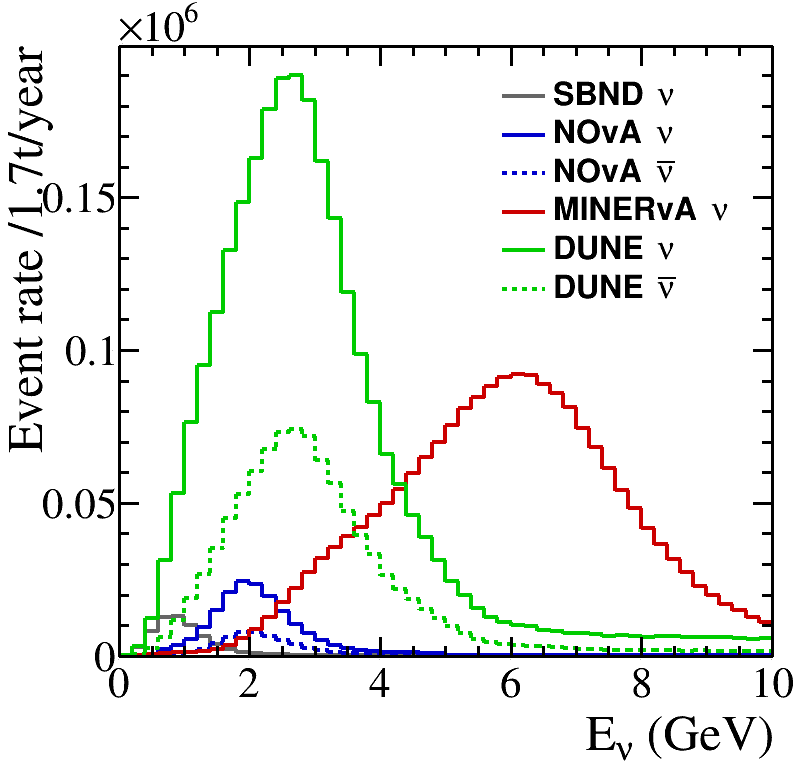
\includegraphics[width=0.5\textwidth]{plots/2x2_Enu_all.png}}
  \caption{Comparison of the absolutely normalized fluxes for different neutrino beamlines at Fermilab, and the expected yearly rates in the ArgonCube 2x2 Demonstrator module's 1.7t active LAr volume as a function of \enu, produced using GENIE v2.12.10 with the ``ValenciaQEBergerSehgalCOHRES'' configuration~\cite{genie}.}
  \label{fig:beam_options}
\end{figure}
In Figure~\ref{subfig:flux}, the currently available neutrino fluxes at various near detector halls in Fermilab are compared, on an absolutely normalized scale, to the LBNF three-horn optimized flux at the 574~m near detector site~\cite{dune_opt_flux}. The currently available neutrino fluxes considered are the on- and 14 mrad. off-axis medium-energy neutrinos from the main injector (NuMI) beam~\cite{numi}, which corresponds to the MINOS and NOvA near detector halls; and the booster neutrino beam (BNB) at the SBND hall~\cite{Antonello:2015lea}. The FY2017 delivered POT was used to produce a yearly flux and rate for the BNB and NuMI beams~\cite{fnal_beam_2017}. It is clear that the proposed LBNF flux is significantly more intense than the fluxes sampled at any existing experimental hall. However, due to the roughly linear relationship between neutrino energy and cross section, the measured rate from the on-axis NuMI beam in the MINOS-ND hall is approximately the same as for the planned LBNF flux, and is therefore the most desirable currently functional experimental hall at Fermilab for a ProtoDUNE-ND test. The rate has been produced with the GENIE neutrino interaction Monte Carlo package~\cite{genie}, using v2.12.10 with the ValenciaQEBergerSehgalCOHRES configuration. Note that the rate is normalized to the active volume of the ArgonCube 2x2 Demonstrator module, showing that significant statistics will be accumulated in a matter of months of ProtoDUNE-ND operation.

\FloatBarrier
\subsection{MINOS near detector hall}
\label{sec:minos-hall}
\begin{itemize}
\item Size of the hall
\item Existing infrastructure required for the test
\item Need to consider whether we need to move anything (e.g. MINERvA) to make space
\item New infrastructure to be put in for the test --> Barry Norris/ Alan Bross. Probably need to discuss language with Steve Brice to make it forceful enough
\end{itemize}

\subsection{ArgonCube 2x2 Demonstrator module}
\label{sec:2x2-design}

ArgonCube, and the Argoncube 2x2 Demonstrator module are described in Ref.~\cite{argoncube_loi}. However, a number of significant changes to the design have been made since then, to account for the advancements made in the ArgonCube R\&D program. In particular, the four modules of the ArgonCube 2x2 Demonstrator module will not test separate technologies, as design choices have already been informed by smaller scale tests. Instead, the modules will be functionally identical, to allow for more sophisticated reconstruction tests.

\begin{figure}[htbp]
\centering
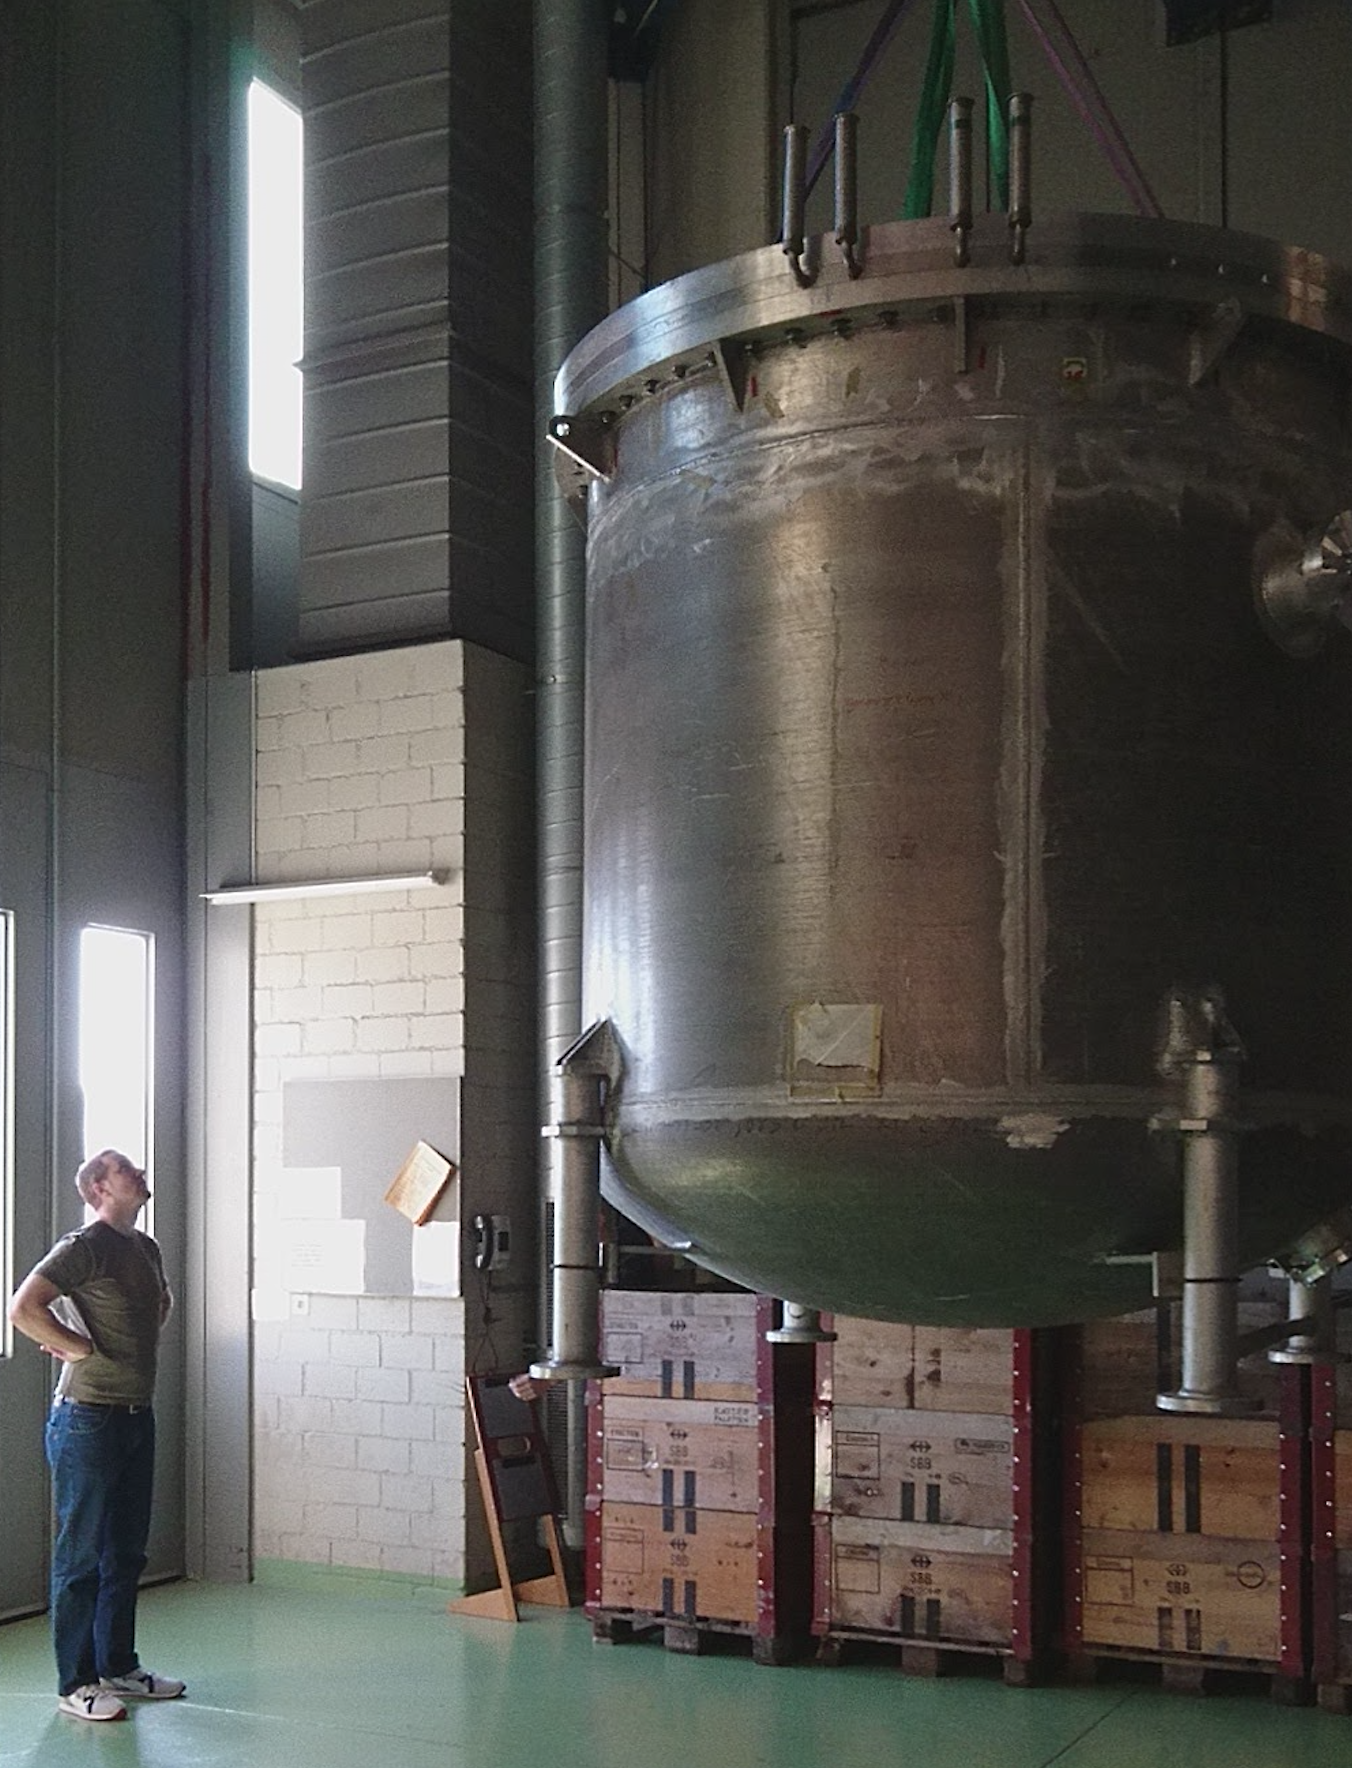
\includegraphics[width=0.45\linewidth]{plots/cryostat.png}
\caption{The liquid nitrogen-cooled and vacuum-insulated cryostat that will host the ArgonCube 2x2 Demonstrator module, reproduced from Ref.~\cite{argoncube_loi}.}
\label{fig:2x2_cryostat}
\end{figure}

The basic principle of ArgonCube is a detector made of self-contained TPC modules sharing a common cryostat. Each module is made of a rectangular box with a square footprint and a height to be optimized in order to meet the physics goals and/or sensitivity constraints. The ArgonCube 2x2 Demonstrator module will be housed within an existing liquid nitrogen (LN2)-cooled and vacuum-insulated cryostat, shown in Figure~\ref{fig:2x2_cryostat}, which is $\sim$\SI{2.2}{\metre} in diameter, and $\sim$\SI{2.8}{\metre} deep, for a total volume of $\sim$\SI{6}{\metre\cubed}. The size of the cryostat sets the dimensions of the modules for the demonstrator. The square base of each module will be \SI{0.67 x 0.67}{\metre}, and the height will be \SI{1.81}{\metre}. This makes the modules comparable in size to, but slightly smaller than, the proposed DUNE near detector, which will have a base of \SI{1 x 1}{\metre}, with a \SI{3.5}{\metre} height; optimized in order to meet the physics goals and sensitivity constraints.

\begin{figure}[htbp]
\centering
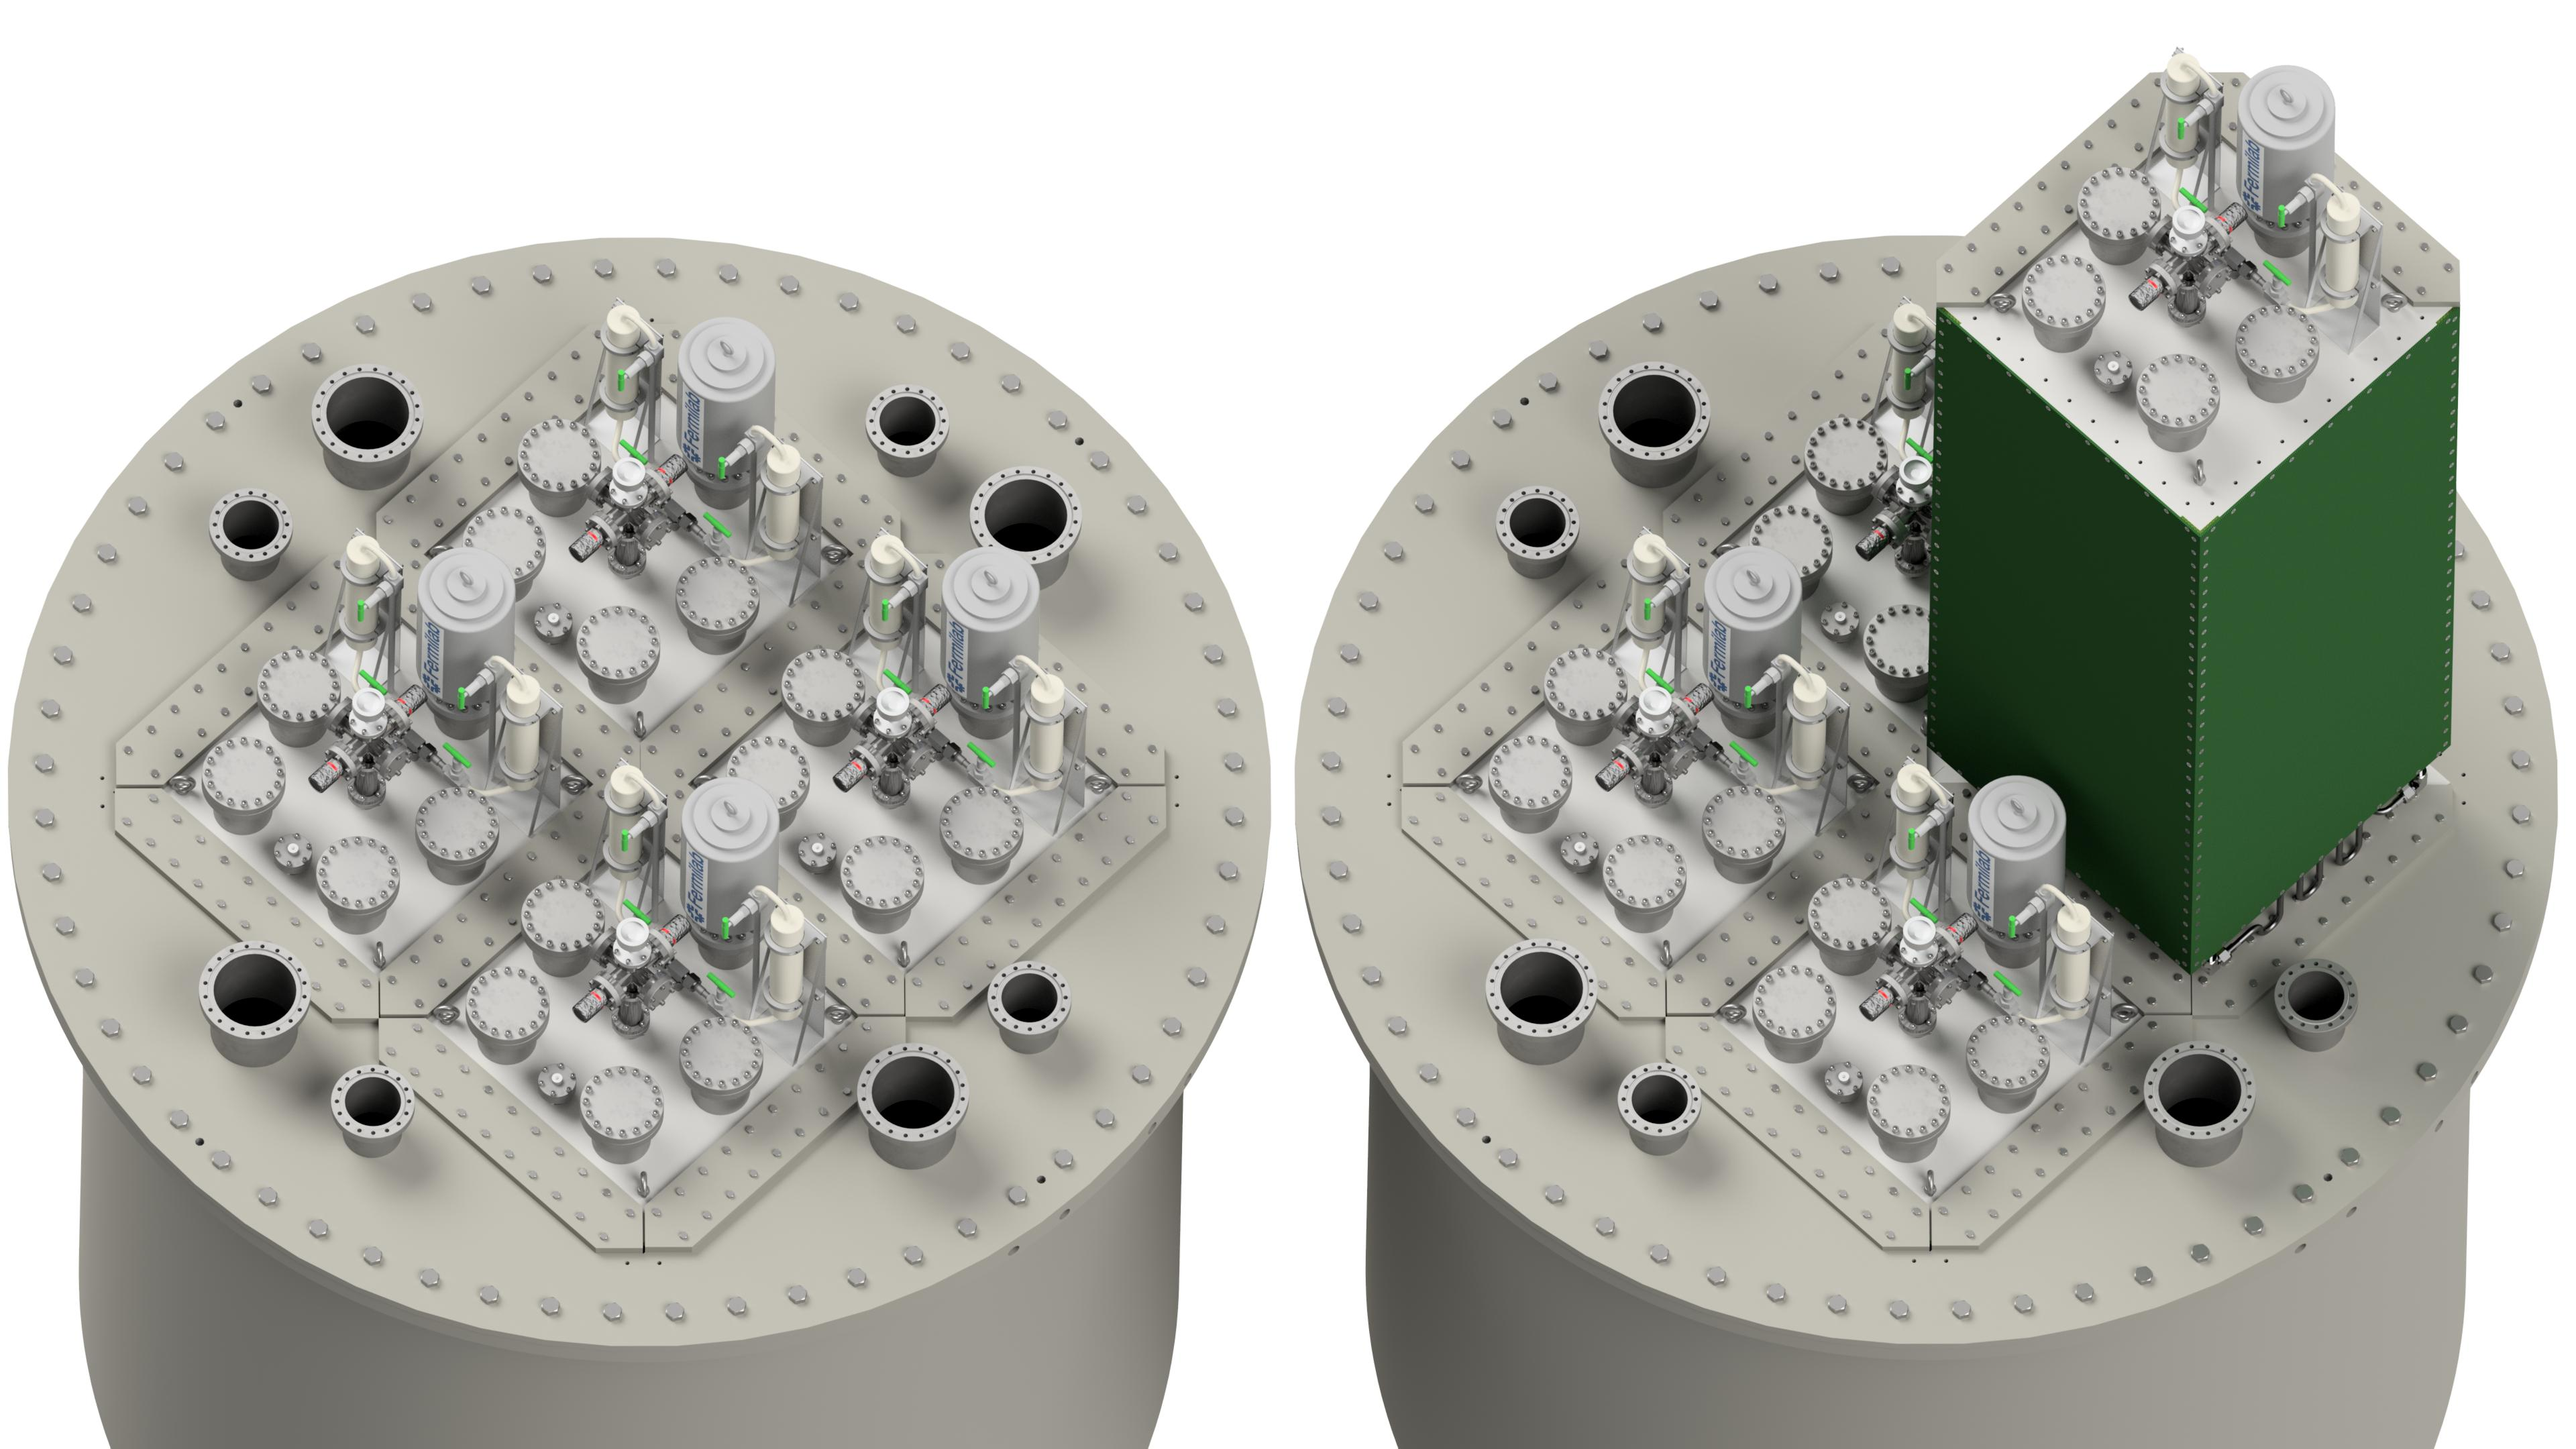
\includegraphics[width=\textwidth]{plots/BathAndModule.png}
\caption{Illustration of the ArgonCube 2x2 Demonstrator module. The four modules are visible, with one of them is partly extracted, on the right. This figure has been reproduced from Ref.~\cite{argoncube_loi}.}
\label{fig:2x2_extraction}
\end{figure}

Individual modules can be extracted or reinserted into a common LAr bath as needed, as is illustrated in Figure~\ref{fig:2x2_extraction}. Pressure inside the modules is kept close to the bath pressure putting almost no hydrostatic force on the module walls, which allows them to be thin, to minimize the inactive material in the walls. The purity of the LAr is maintained within each module independently, as will be described below. As a result, the argon surrounding the modules needs not meet as stringent purity requirements as the argon inside. Under normal operation conditions all modules are inserted with only clearance distances between modules. Cooling power to the bath is supplied by cryocoolers located in unistrumented volumes at the side of the detector called service volumes, and LN2 circulated through lines on the outer surface of the inner cryostat vessel.

\begin{figure}[tbp]
  \centering
  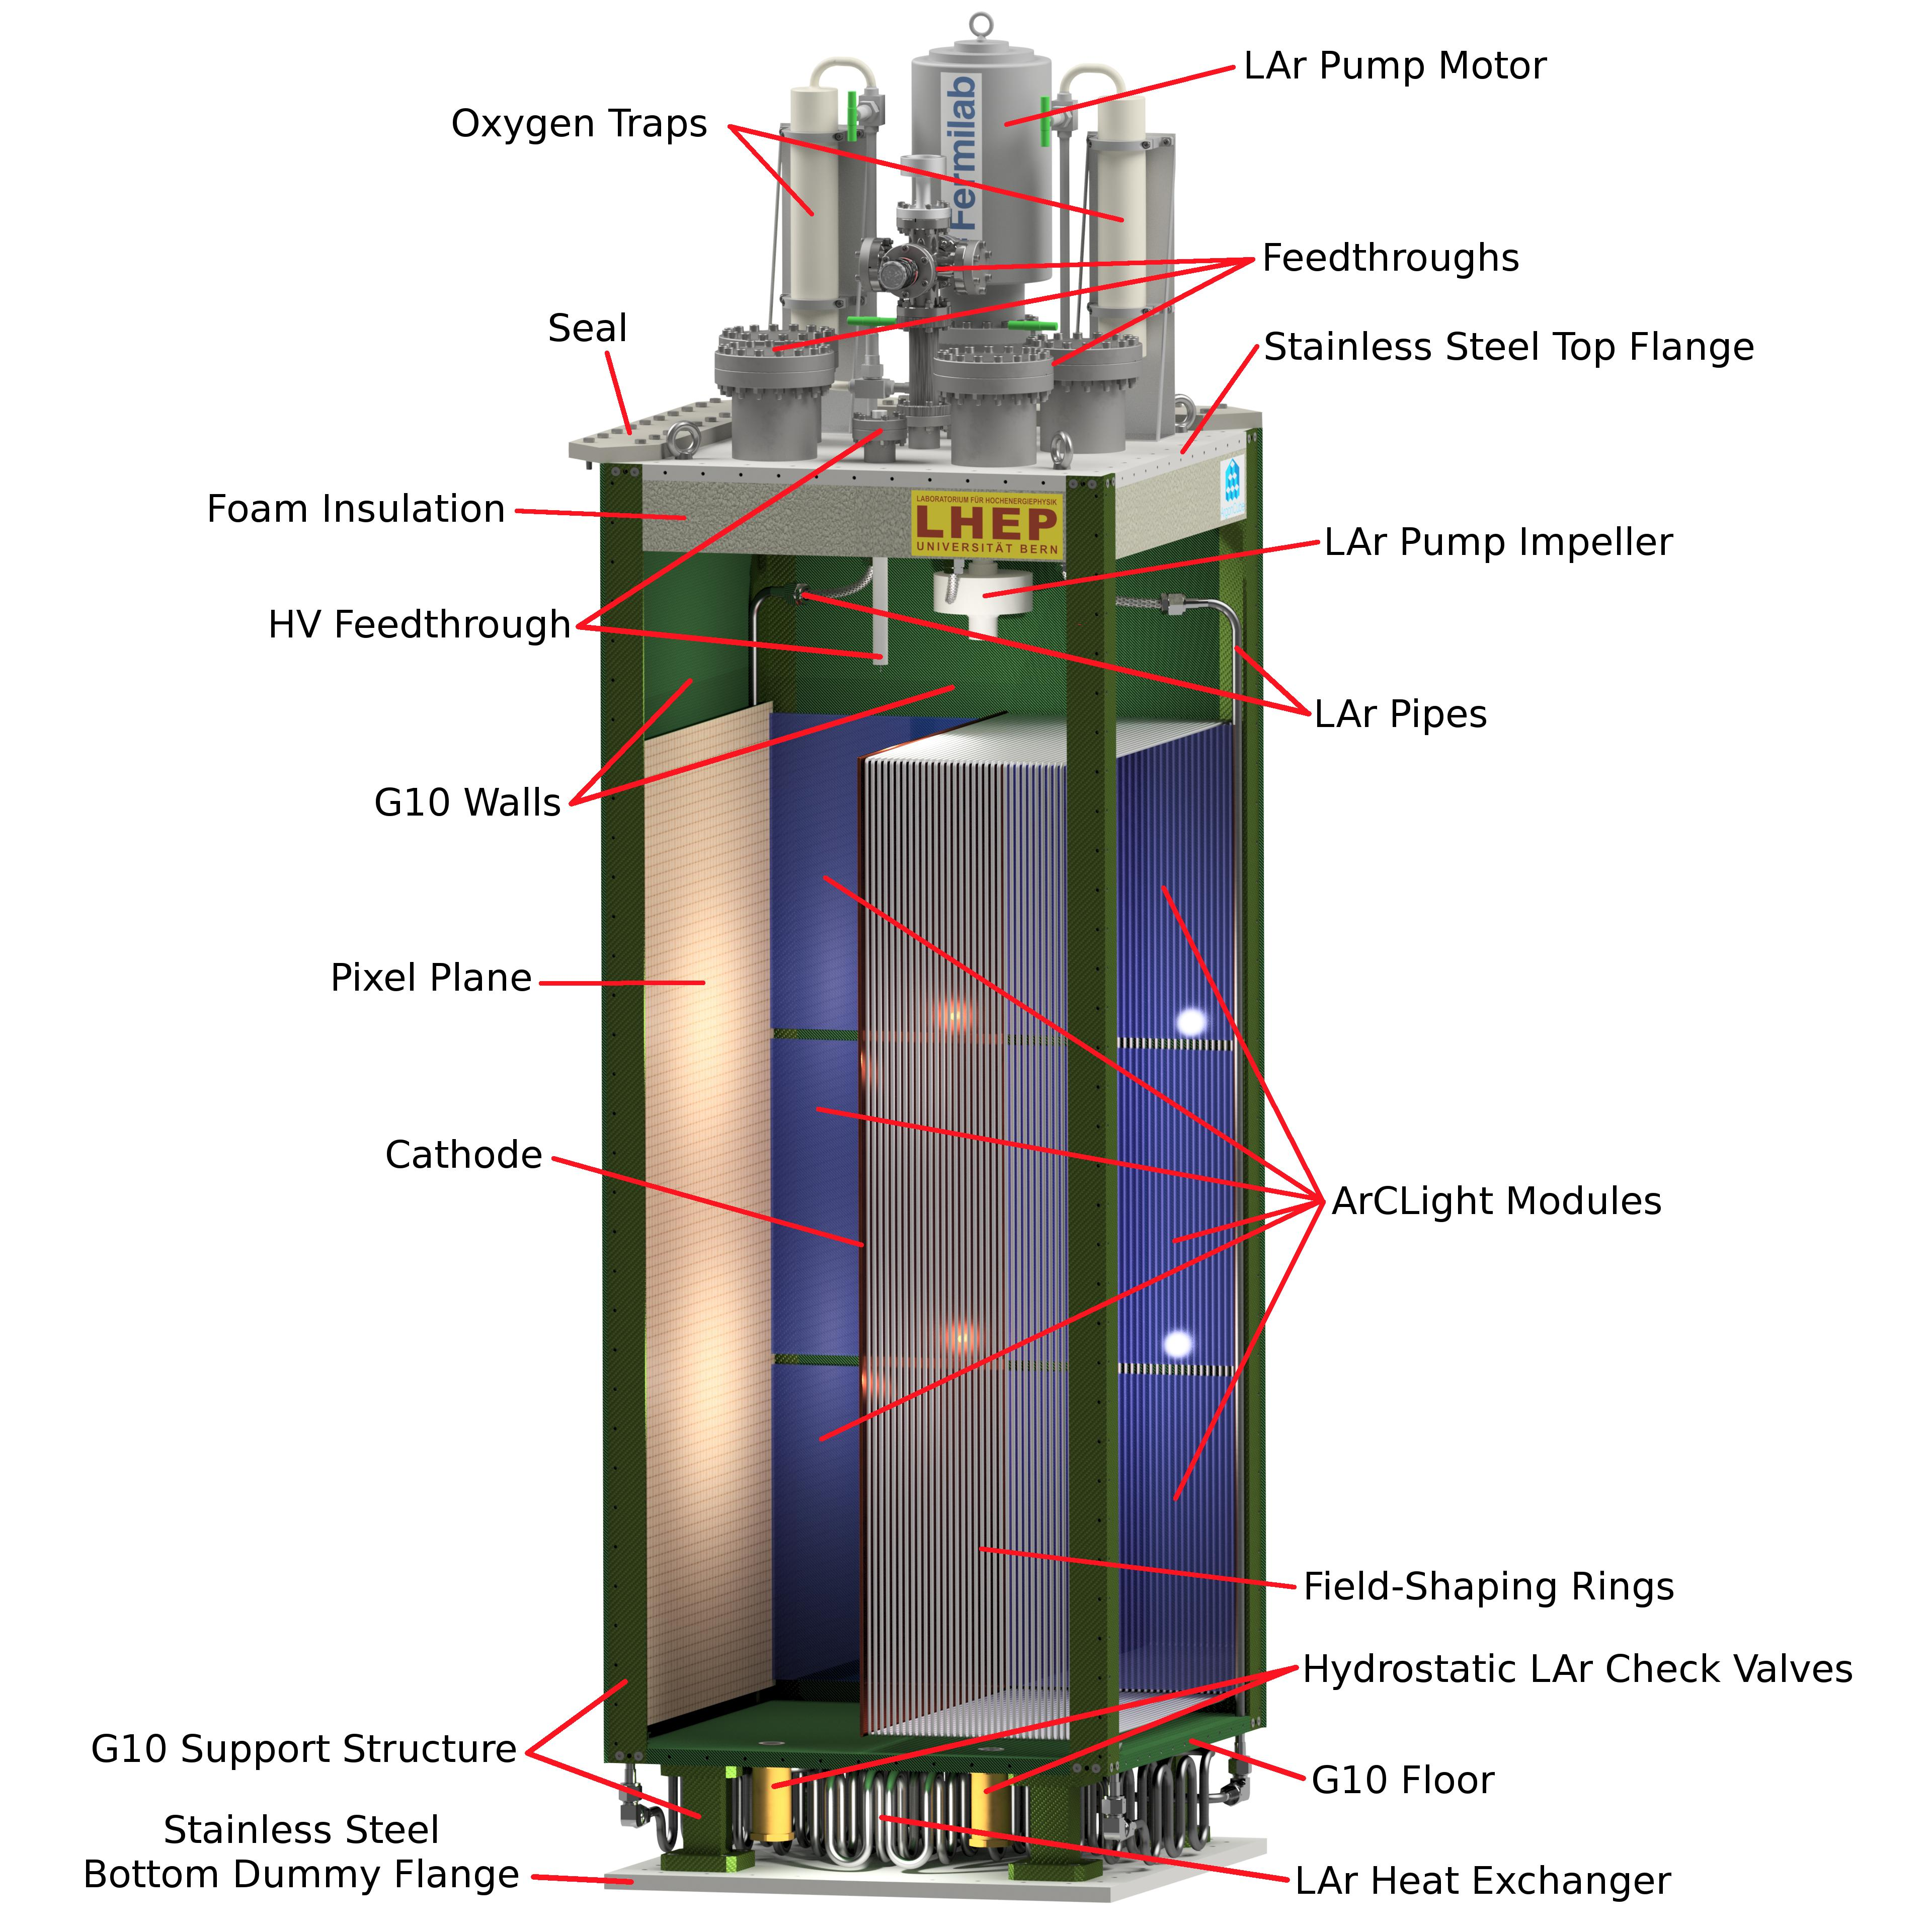
\includegraphics[width=0.8\textwidth]{plots/Normal-Module-4K_labelled.png}
  \caption[ArgonCube module engineering drawing]{Cutaway drawing of a \SI{0.67 x 0.67 x 1.81}{\metre} ArgonCube module for the 2x2 Demonstrator module. For illustrative purposes the drawing shows traditional field shaping rings instead of a resistive field shell. Note, G10 walls will completely seal the module, isolating it from the neighbouring modules and the outer liquid argon bath.}
  \label{fig:ac_module}
\end{figure}

A cutaway drawing of an individual 2x2 module is shown in Figure~\ref{fig:ac_module}. The side walls of each module are made from \SI{1}{\centi\metre} G10 sheets, to which the resistive field shell is laminated. G10's electromagnetic radiation length ($X_{\mathrm{0}} = \SI{19.4}{\centi\metre}$) and hadronic interaction length ($\lambda_{\mathrm{int}} = \SI{53.1}{\centi\metre}$)~\cite{pdg_g10} are both comparable to LAr (14.0~cm and 83.7~cm respectively), making G10 structures in LAr almost transparent for passing particles, allowing for a performance comparable to a monolithic detector. G10 provides a strong dielectric, capable of \SI{200}{\kilo\volt\per\centi\metre} at \SI{1}{\centi\metre} thick~\cite{G10Breakdown}. This dielectric shielding eliminates the need for a clearance volume between the TPCs and the cryostat, while also shielding the TPC from field breakdowns in a neighbouring module. 

The module is split into two TPCs by a central cathode made of an additional resistive layer on a G10 substrate. The segmented drift length does not require a high cathode voltage, and minimizes stored energy. For the 2x2 module footprint of \SI{0.67 x 0.67}{\metre} and an electric field of \SI{1}{\kilo\volt\per\centi\metre} a cathode potential of only \SI{33}{\kilo\volt} is required. The HV is brought into the module using a commercially available feedthrough. Operating a LArTPC at this voltage is challenging, but feasible, without a prohibitive loss of active volume~\cite{argontube}.

The detector is oriented such that the cathodes are parallel to the beam. This minimizes the load on the readout electronics by spreading the event over more channels and reducing the required digitization rate for hit channels. In turn, this reduces the heat load generated at the charge readout and prevents localized boiling.


During module insertion and extraction, the argon flow is controlled by hydrostatic check valves located at the module bottom, which require a minimal differential pressure to open. Purity inside each module is maintained by means of continuous LAr recirculation through oxygen traps. Dirty argon is sucked in at the module top and then pushed through the oxygen traps, clean argon is first routed through a heat exchanger, located below the module inside the outer bath, for cooling and then re-enters the module at the base of the active volume. For optimal heat transport the argon flow is directed along the cold electronics. To prevent dirty argon from the bath entering the modules their interior is held at a slight overpressure, just below the opening pressure of the check valves. For the 2x2 Demonstrator each module will have its own pump and filters, this will not be the case for the ND. In the ND, a more extensive LAr infrastructure will be employed with LAr extracted and filtered in a plant separate to the detector.  

ArgonCube offers true 3D tracking information using the LArPix pixelated charge readout and cryogenic electronics~\cite{larpix}, which are used to amplify and digitize the single-pixel signals in the cold to avoid any analogue multiplexing, and produce unambiguous 3D information. Pixelated anode planes are located on the two module walls parallel to the cathode. The baseline design is for a 5 mm pixel pitch. The LArPix electronics, and a summary of their associated R\&D work, are described in Ref.~\cite{larpix}.

\begin{figure}[!ht]
\centering
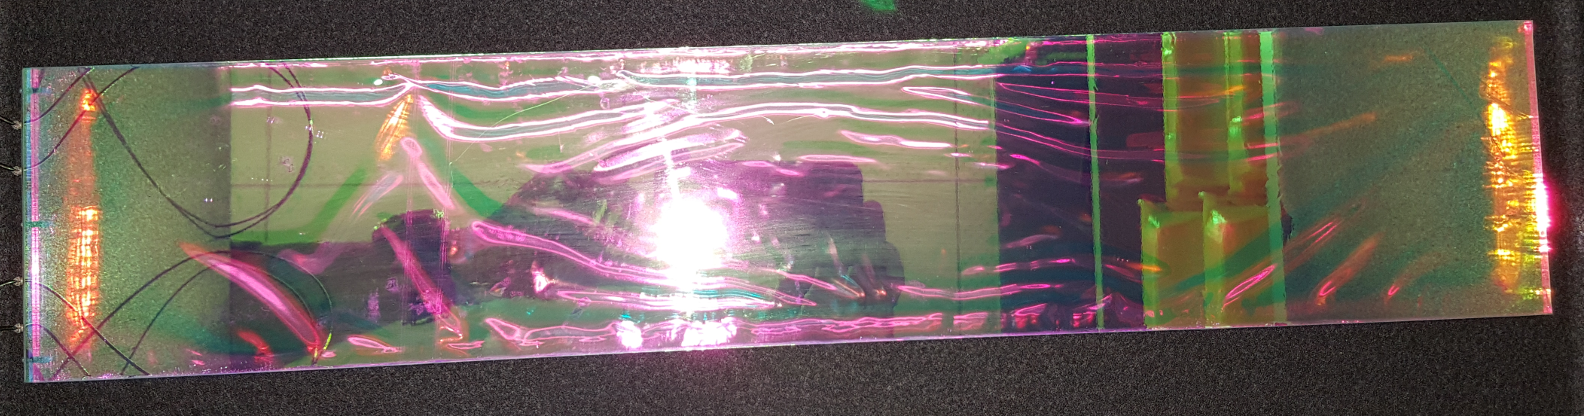
\includegraphics[width=0.75 \linewidth]{plots/1Film50x10.png}
\caption{A prototype ArgonCube light readout paddle built at the University of Bern. The paddle is 50~cm long and 10~cm wide, with four SiPMs coupled to one end. Reproduced from Ref.~\cite{argoncube_loi}.}
\label{fig:arclight}
\end{figure}

With LArPix, the reconstruction issues in a high rate environment are drastically simplified with respect to traditional projective wire readout TPCs. However, the charge readout window (drift time) is \SI{137}{\micro\second} and the beam spill is \SI{10}{\micro\second}, so to correctly reconstruct events overlapping in this window, scintillation signals need to be correctly matched to charge signals (flash matching). If these are correctly matched, the prompt scintillation light defines the time at which ionization electrons start to drift, and the time it takes to register charge on the anode plane along with the electric field strength allow give you enough information to reconstruct the third spatial co-ordinate (along the drift direction). In a modular detector, this problem can easily be simplified using an opaque cathode and module walls, which contains scintillation light in each TPC (half module), and effectively reduce the event pile-up. Furthermore, attenuation due to Rayleigh scattering, $6.6\times10^{-1}$~m~\cite{Rayleigh}, is much less of a problem than in large monolithic detectors given maximum photon propagation distances of only \SI{0.3}{\metre}. It is desirable to have a large area photon detection system to maximize the utility of scintillation light signals in the detector. However, the downside to modularization is the dead regions between adjacent TPCs, which introduce gaps in the reconstruction, so any light detection system must be compact. The solution pursued for the ArgonCube effort is ArCLight~\cite{arclight}, which is a very compact dielectric light trap that allows for light collection from a large area, inside high electric fields. An example ArCLight sheet is shown in Figure~\ref{fig:arclight}. These sheets are mounted on the walls of the module, inside the field shell, aligned with the drift direction, between the anode and the cathode. The additional dead volume of a few \si{\milli\metre} is similar to the one caused by the charge readout in the perpendicular direction.


\todo{James, can you comment on the 2x2 needs from the external infrastructure point of view?}

\subsection{Downstream tracking detectors}
\label{sec:tracking_detectors}
As well as an ArgonCube-like LAr component, the recommendations from the DUNE Near Detector Concept Study Group~\cite{dune_ndcsg} are for there to be additional, downstream tracking detectors in the DUNE ND to tag and measure the energies of particles which exit the downstream face of the LAr detector, and a magnetized component to identify the sign of muons (and other particles). It would therefore enhance the utility of ProtoDUNE-ND, as an intermediate-scale test of the DUNE ND, to include prototypes for these detectors. It would also enhance any additional possible physics outputs from ProtoDUNE-ND, as many events in the high-energy NuMI ME beamline will not be fully contained in the ArgonCube 2x2 Demonstrator module (examples can be seen in Figures~\ref{fig:argonbox_event_display} and~\ref{fig:leaky_event}). Two downstream tracking options considered  by the DUNE Near Detector Concept Study Group are the Three Dimensional Scintillator Tracker (3DST), and the High-Pressure gaseous argon TPC (HPgTPC).

The 3DST is a fully active plastic scintillator detector made of a large number of optically independent 1x1x1 cm$^{3}$ cubes read out in three orthogonal directions by wavelength shifting fibers~\cite{3dst}. The 3DST is envisioned as an upgrade to the plastic scintillator detectors read out in two dimensions used by T2K~\cite{t2k-fgd,t2k-ingrid}, NOvA~\cite{nova} and MINERvA~\cite{minerva-nim}, which will provide better angular resolution. Unfortunately, after consultation with the 3DST steering group, it was found that a large scale prototype suitable for ProtoDUNE-ND will not be available on the required timescale. If the situation changes, we note the desirability of including such a prototype in the proposed ProtoDUNE-ND effort.

The HPgTPC is a high-pressure argon gas TPC which will operate inside a magnetic field~\cite{dune_ndcsg}. Its purpose is two-fold. Firstly, it acts as a downstream tracker for particles exiting the LAr detector, with a superior dE/dx resolution, and the ability to measure the sign and momentum of particles in the magnetic field. Secondly, it offers a lower threshold, higher resolution argon target detector than the LAr component, which may help constrain certain aspects of the model. The HPgTPC needs to be coupled with a further downstream ECal to detect escaping photons, and to provide fast timing to differentiate tracks from multiple interactions. Although a HPgTPC prototype is not ready at the time of writing this proposal, it is expected that a prototype will be produced during ProtoDUNE-ND operation, so the program should be flexible enough to incorporate a new detector component. A downstream ECal is required for the HPgTPC in order to provide fast timing to differentiate different interactions, and to detect photons which will not convert in the argon gas.

As all potential DUNE ND designs identified in Ref.~\cite{dune_ndcsg} include a fast scintillator component, and a 3DST module will not be available on the timescale of ProtoDUNE-ND, it is desirable to see whether elements of the existing MINERvA detector in the NuMI hall can be re-purposed, as the MINERvA experiment will stop taking data in summer 2019, before ProtoDUNE-ND will get underway. This possibility is discussed separately in Section~\ref{sec:MINERvA}, following discussions with members of MINERvA who have expressed an interest in joining the ProtoDUNE-ND effort.

As it is expected that the ProtoDUNE-ND setup may need to be reconfigured, with the addition of more components over time, and because DUNE-PRISM is now the baseline ND design, it is desirable to include a moveable cryogenic system for the ArgonCube 2x2 Demonstrator in ProtoDUNE-ND, which would allow the future moveable cryogenics for DUNE-PRISM to be tested.


\section{ProtoDUNE-ND detector physics studies}
\label{sec:detector-physics-studies}
Basic detector stability checks will be performed with a period of detector operation in Bern before moving the ArgonCube 2x2 Demonstrator module to Fermilab. These tests will include extraction and re-insertion tests of individual modules into the LAr bath, and checks that the LAr purity is sufficient. However, local tests can only be performed using cosmic muons, which have limited utility beyond basic detector stability checks. In this section, we identify a number of key detector physics questions which could be answered by the ProtoDUNE-ND test, and would help inform the final design of the DUNE ND, and aid in developing reconstruction algorithms suitable for neutrino interactions.

In order to check the feasibility of these studies, two different simulations were used. Firstly, high statistics GENIE Monte Carlo samples were produced, in order to compare basic properties of neutrino interactions expected in the LBNF and NuMI ME beamlines. Secondly, GENIE events were used to seed a basic GEANT4 simulation, using the ArgonBox\footnote{\url{https://github.com/dadwyer/argon_box}} software, in order to get a basic understanding of event shape and containment. In the latter simulation, events were simulated in a very large (200 m $\times$ 200 m $\times$ 200 m) box of LAr, and were then distributed randomly inside a volume with the correct spatial dimensions of the ArgonCube 2x2 Demonstrator module. Although the 2x2 geometry was not included in the simulation, this gives an acceptable estimate of the expected event rates and containment for the studies described below, as these do not depend significantly on the detailed geometry of the detector. Note that for all ArgonBox studies shown here, the NuMI on-axis forward horn current (neutrino-enhanced) beam was used. Examples of the ArgonBox simulation with the basic ArgonCube 2x2 Demonstrator geometry superimposed can be seen in Figure~\ref{fig:argonbox_event_display} for a number of different neutrino energies.

\begin{figure}[htb]
  \centering
  \subfloat[$E_{\nu}$ = 2.60 GeV] {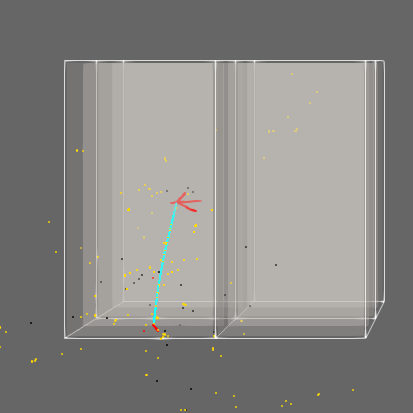
\includegraphics[width=0.45\textwidth]{{plots/EventDisplays/2.60GeV_square_crop}.png}}\hspace{25pt}
  \subfloat[$E_{\nu}$ = 3.36 GeV] {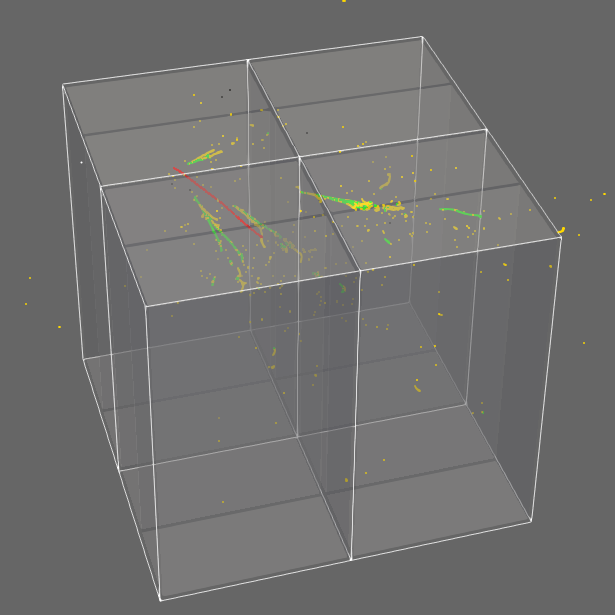
\includegraphics[width=0.45\textwidth]{{plots/EventDisplays/3.36GeV_square_crop}.png}}\\
  \subfloat[$E_{\nu}$ = 4.83 GeV] {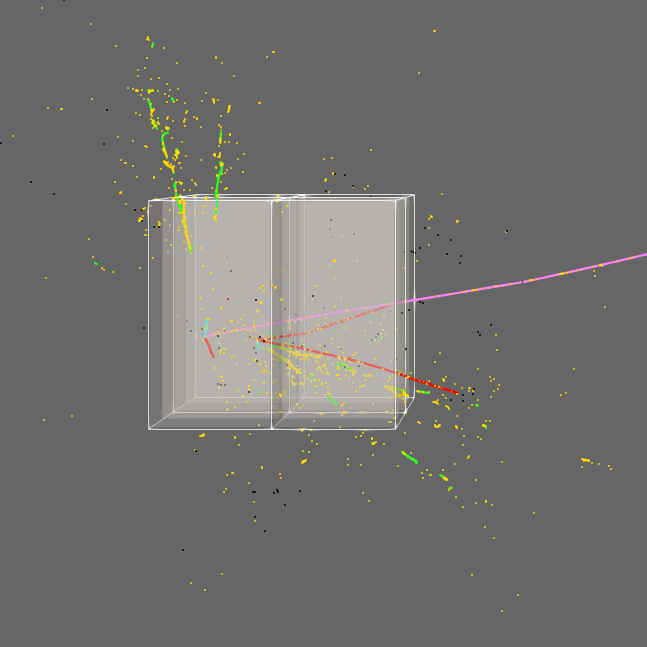
\includegraphics[width=0.45\textwidth]{{plots/EventDisplays/4.83GeV_square_crop}.png}}\hspace{25pt}
  \subfloat[$E_{\nu}$ = 9.37 GeV] {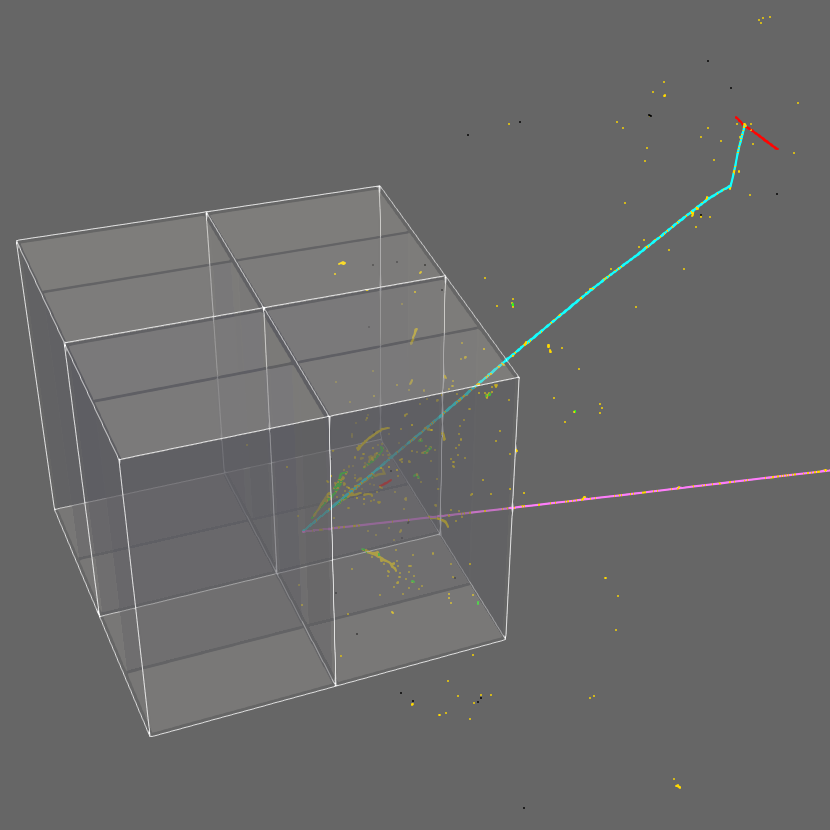
\includegraphics[width=0.45\textwidth]{{plots/EventDisplays/9.37GeV_square_crop}.png}}
  \caption{Example $\nu_{\mu}$--argon ArgonBox simulated events for a number for different incident neutrino energies, where the energy deposits in a bulk volume of LAr are color-coded according to the particle type: $\pi^{\pm}$ --- blue; $\mu^{\pm}$ --- purple; $e^{+}$ --- green; $e^{-}$ --- yellow; proton --- red; recoiling nuclei --- black. The event vertices are randomly placed within the active volume of the 2x2 Demonstrator module, the geometry for which is superimposed on these images, but which is not simulated by ArgonBox.}
  \label{fig:argonbox_event_display}
\end{figure}

The example event displays shown in Figure~\ref{fig:argonbox_event_display} give a basic idea of how NuMI ME energy events (in FHC) would look in the ArgonCube 2x2 Demonstrator module. Although many of the tracks and showers are not contained, some fraction are, which is discussed in more detail for the detector physics studies described below. It also suggests that some fraction of the events seen in the ArgonCube 2x2 Demonstrator module would be fully contained in the active volume, or fully contained except for the outgoing muon, which may open the way for some interesting physics studies beyond the detector physics described in this document. However, any possible utility in this direction would be severely limited without a downstream tracker to contain higher momentum hadronic components, and to tag the muon. This makes the case for adding an additional ProtoDUNE-ND test module for a HPTPC downstream tracker even stronger, or if that proves not to be possible on the timescale of this test, utilizing parts of the existing MINERvA or MINOS-ND detectors in the experimental hall as is described in Section~\ref{sec:MINERvA_MINOS}.

\begin{figure}[htb]
  \centering
  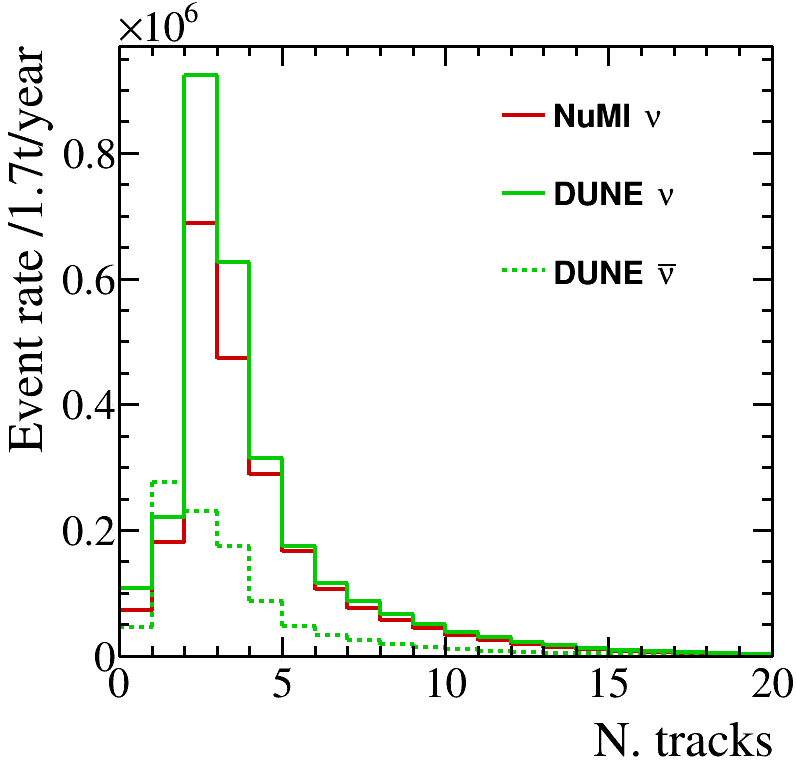
\includegraphics[width=0.5\textwidth]{plots/2x2_ntracks_all.png}
  \caption{The expected yearly rates of minimum and highly ionizing particles expected in the 2x2 Demonstrator module's 1.7t LAr volume for the NuMI ME and LBNF fluxes, produced using GENIE v2.12.10 with the ``ValenciaQEBergerSehgalCOHRES'' configuration~\cite{genie}.}
  \label{fig:track_multiplicity}
\end{figure}
In order to be a relevant test for the full ArgonCube near detector, which will be in the LBNF beamline, it is useful to verify that the basic properties of the events are similar, despite the NuMI ME beam being somewhat higher energy than the planned LBNF beam (as shown in Figure~\ref{fig:beam_options}). Figure~\ref{fig:track_multiplicity} shows the expected multiplicity of minimum or highly ionizing tracks at the vertex for both the LBNF and NuMI ME beams, in neutrino and antineutrino mode, produced with the GENIE generator. The track multiplicities are similar, which indicates that the scale of the reconstruction problem is similar, and the proposed ProtoDUNE-ND test will be a useful benchmark for developing the ArgonCube reconstruction software.

\begin{figure}[htb]
  \centering
  \subfloat[$\mu^{\pm}$] {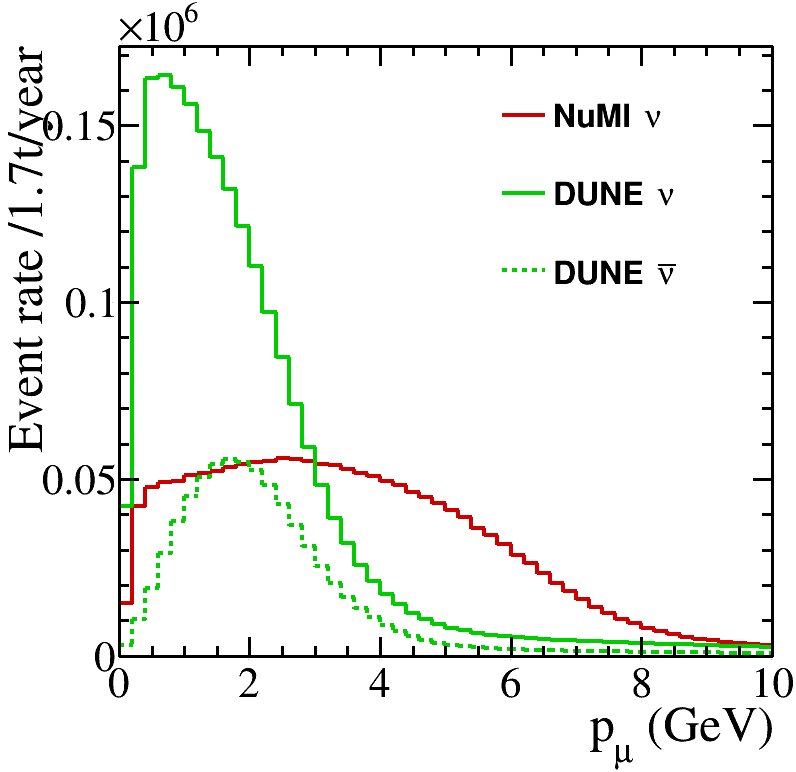
\includegraphics[width=0.5\textwidth]{plots/2x2_muon_mom_all.png}}
  \subfloat[Protons]    {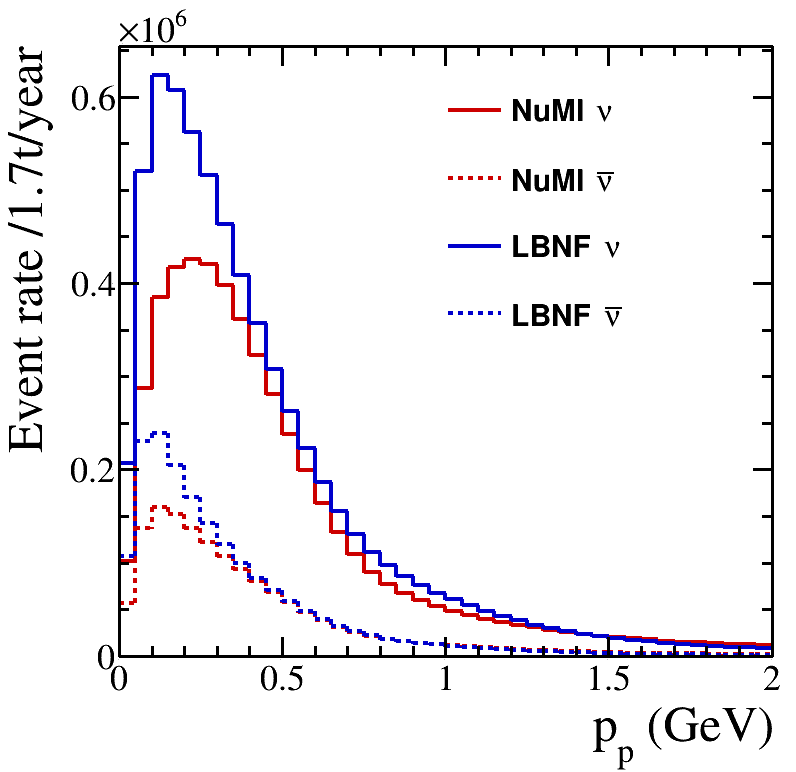
\includegraphics[width=0.5\textwidth]{plots/2x2_proton_mom_all.png}}\\
  \subfloat[$\pi^{+}$]   {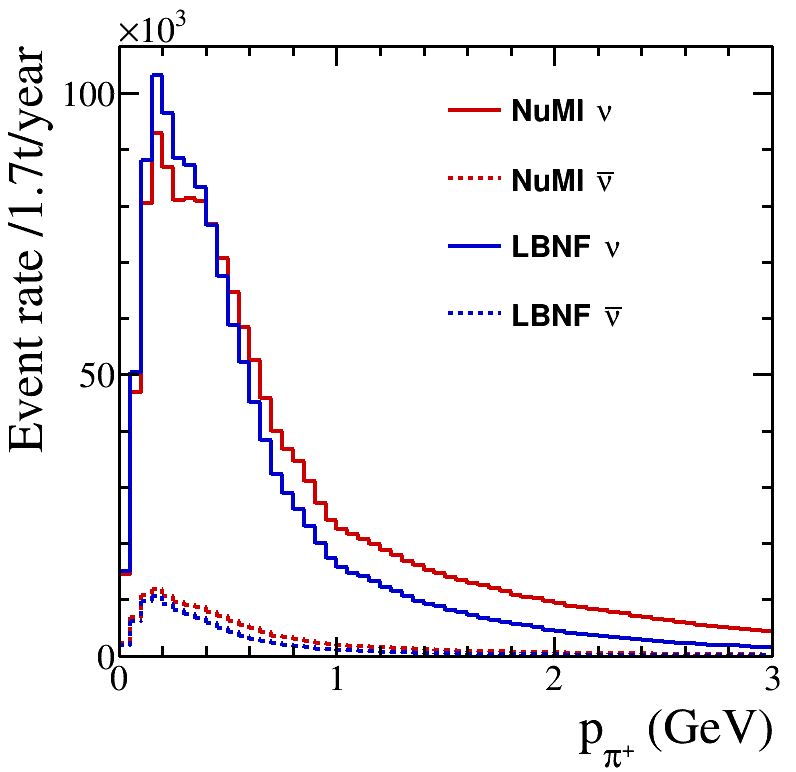
\includegraphics[width=0.5\textwidth]{plots/2x2_piplus_mom_all.png}}
  \subfloat[$\pi^{-}$]   {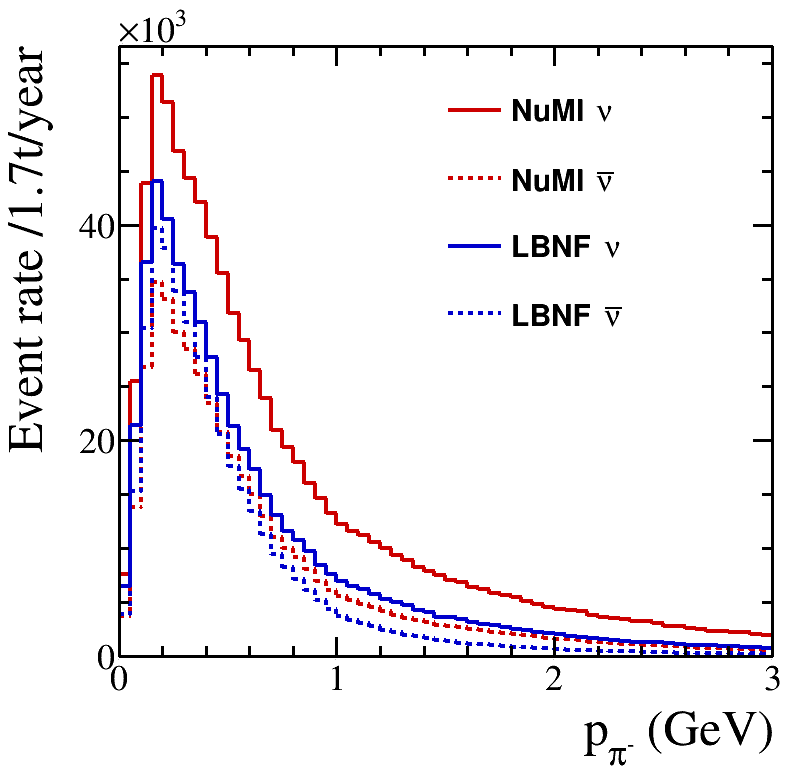
\includegraphics[width=0.5\textwidth]{plots/2x2_piminus_mom_all.png}}  
  \caption{The expected yearly rates of various particles produced at the vertex, as a function of their momentum, expected in the 2x2 Demonstrator module's 1.7t LAr volume for the NuMI ME and LBNF fluxes, produced using GENIE v2.12.10 with the ``ValenciaQEBergerSehgalCOHRES'' configuration~\cite{genie}. Note that every relevant particle from each event is included.}
  \label{fig:momenta}
\end{figure}
In Figure~\ref{fig:momenta}, the momenta of various particles coming from the initial neutrino--argon vertex are compared for the LBNF and NuMI ME beams. As expected, the energy distributions of all of the particles are slightly broader for the NuMI ME flux, but there are significant numbers of events in the NuMI sample which have particle kinematics typical of the LBNF sample. The NuMI sample would therefore be an efficient tool for studying the performance of the ArgonCube detector in the LBNF beam.

In the full 7 $\times$ 5 module ArgonCube detector and the more intense LBNF beamline, with $\sim$14.7 interactions per \SI{10}{\micro\second} beam spill makes for a very high-multiplicity environment. The entire spill will effectively occur instantaneously in the \SI{220}{\micro\second} drift window. Issues with tracks overlapping from separate neutrino interactions are mitigated by the fully-3D readout, but association of all hits to a specific neutrino interaction can still be challenging. For charged tracks, which are spatially connected to their respective neutrino interaction vertices, this association is straightforward.  However, many events contain photons and neutrons, which produce significant energy deposits that are detached from the rest of the event, and may even occur in a different ArgonCube module. Here, the ArCLight light-readout system, with the ability to measure prompt scintillation light with nanosecond resolution, will play a crucial role to associate particle tracks with the correct interaction vertices. Additionally, the relatively small size of the ArgonCube 2x2 Demonstrator module means that relatively few of the tracks will be contained, making particle identification (PID) studies challenging, except for the cases listed below. Although other detectors are not included in the ArgonBox simulation, the lack of containment and PID capabilities mean that including another subdetector in the ProtoDUNE-ND setup is essential for any detector response measurements as a function of charge or momentum.


\subsection{Combining light and charge signals}
An important challenge is to develop automated event reconstruction software with the ArgonCube detector. The pixel readout removes the ambiguities present for projective wire readout TPCs, but the reconstruction software for the latter has benefited from several years of development for the MicroBooNE~\cite{microboone} and ICARUS experiments~\cite{icarus}. Although strides forward for pixel readout TPCs have been made in the PixLAr experiment (where pixel planes were introduced to the LArIAT experiment~\cite{lariat}), the reconstruction problem for charge particle scattering in a small TPC is much simpler than for the ProtoDUNE-ND or DUNE ND environments. Additionally, the reconstructed track position along the drift direction, and the suppression of cosmic backgrounds within the beam window, will be performed using information from the ArcLight light collection system. Checking that the light and charge signals can be combined in the full-size ArgonCube modules, in a comparably noisy environment to the DUNE ND, is an essential test of the ArgonCube design.

\subsection{Neutron identification}
\label{sec:2x2_neutron}
Neutrons present a particular challenge for neutrino energy reconstruction in DUNE and other long-baseline neutrino oscillation experiments. Neutrino oscillations are a function of neutrino energy, but this cannot be reconstructed on an event by event basis because neutrons carry away some fraction of the energy, and are not directly observable. Figure~\ref{fig:neutron_kinematics} shows the expected neutron rate as a function of multiplicity and momentum for the LBNF and NuMI ME beamlines.
\begin{figure}[htb]
  \centering
  \subfloat[Neutron multiplicity]   {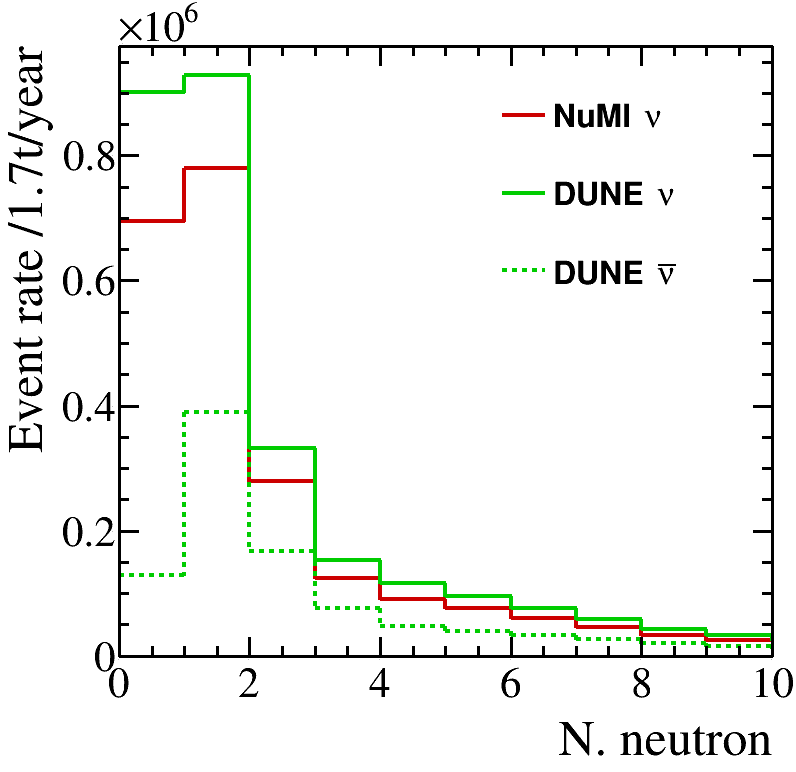
\includegraphics[width=0.5\textwidth]{plots/2x2_nneutron_all.png}}
  \subfloat[Neutron momentum]       {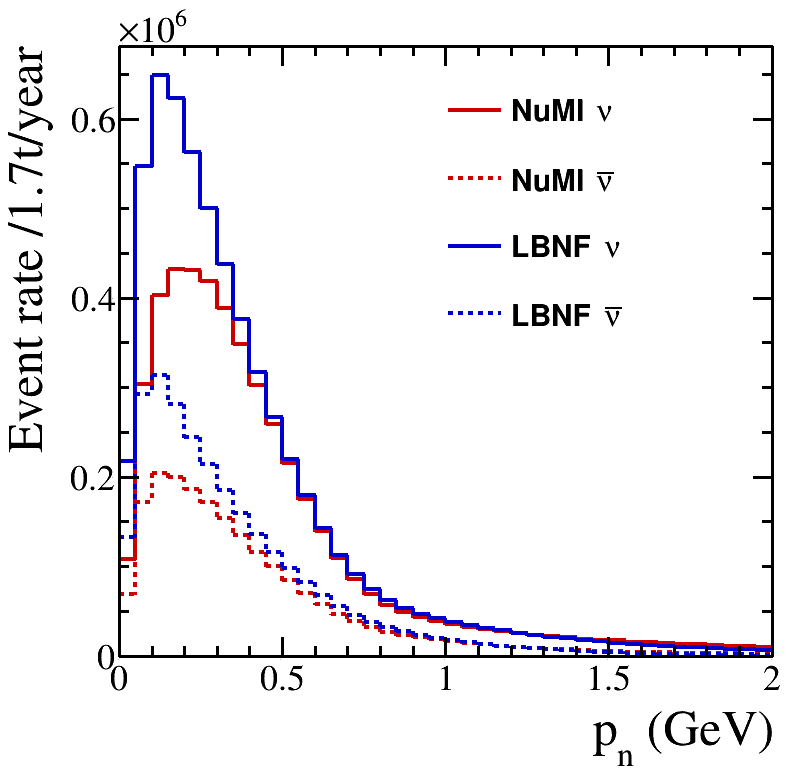
\includegraphics[width=0.5\textwidth]{plots/2x2_neutron_mom_all.png}}  
  \caption{The expected yearly rates of neutrons produced at the vertex, as a function of event multiplicity and their momentum, expected in the 2x2 Demonstrator module's 1.7t LAr volume for the NuMI ME and LBNF fluxes, produced using GENIE v2.12.10 with the ``ValenciaQEBergerSehgalCOHRES'' configuration~\cite{genie}. Note that every neutron from each event is included in the momentum distribution.}
  \label{fig:neutron_kinematics}
\end{figure}

There are two possible ways to identify the presence of neutrons in an event:
\begin{enumerate}
\item Detection of slow neutrons with kinetic energies of $\mathcal{O}$~keV through neutron capture. This is usually achieved by applying a neutron affine coating, e.g. gadolinium, to the detector walls. The radiation emitted from excited nuclei after having captured a neutron is interaction-specific and thereby serves as an indicator for slow neutrons.
\item Detection of fast neutrons with kinetic energies from $\mathcal{O}$~1 MeV-- 1 GeV through recoiling charge particles after a collision of a neutron with a nucleus. The recoiling particle can be the nucleus as a whole, or, if the neutron exceeds the nuclear binding energy ($\sim$~5~MeV for an argon nucleus), a knock-out proton or heavier nuclear fragments like deuterons.
\end{enumerate}
For oscillation experiments, fast neutrons are a much greater issue, as they may carry away a significant fraction of the neutrino energy in an event. It is, therefore, of great interest to investigate the potential of LAr experiments to tag these missing neutron with neutron-induced recoils. Investigating the neutron tagging rate in ProtoDUNE-ND will provide useful information for DUNE sensitivity studies as it will in the ProtoDUNE-ND, this provides an opportunity to investigate how well charge and light signals can be combined.

The values for pixel pitch and ArCLight threshold used in the following studies are taken from the DUNE ND proposal~\cite{argoncube_loi}, although not identical to the 2x2, they are sufficiently close for the purpose of this work.  

\begin{figure}[htbp]
  \centering
  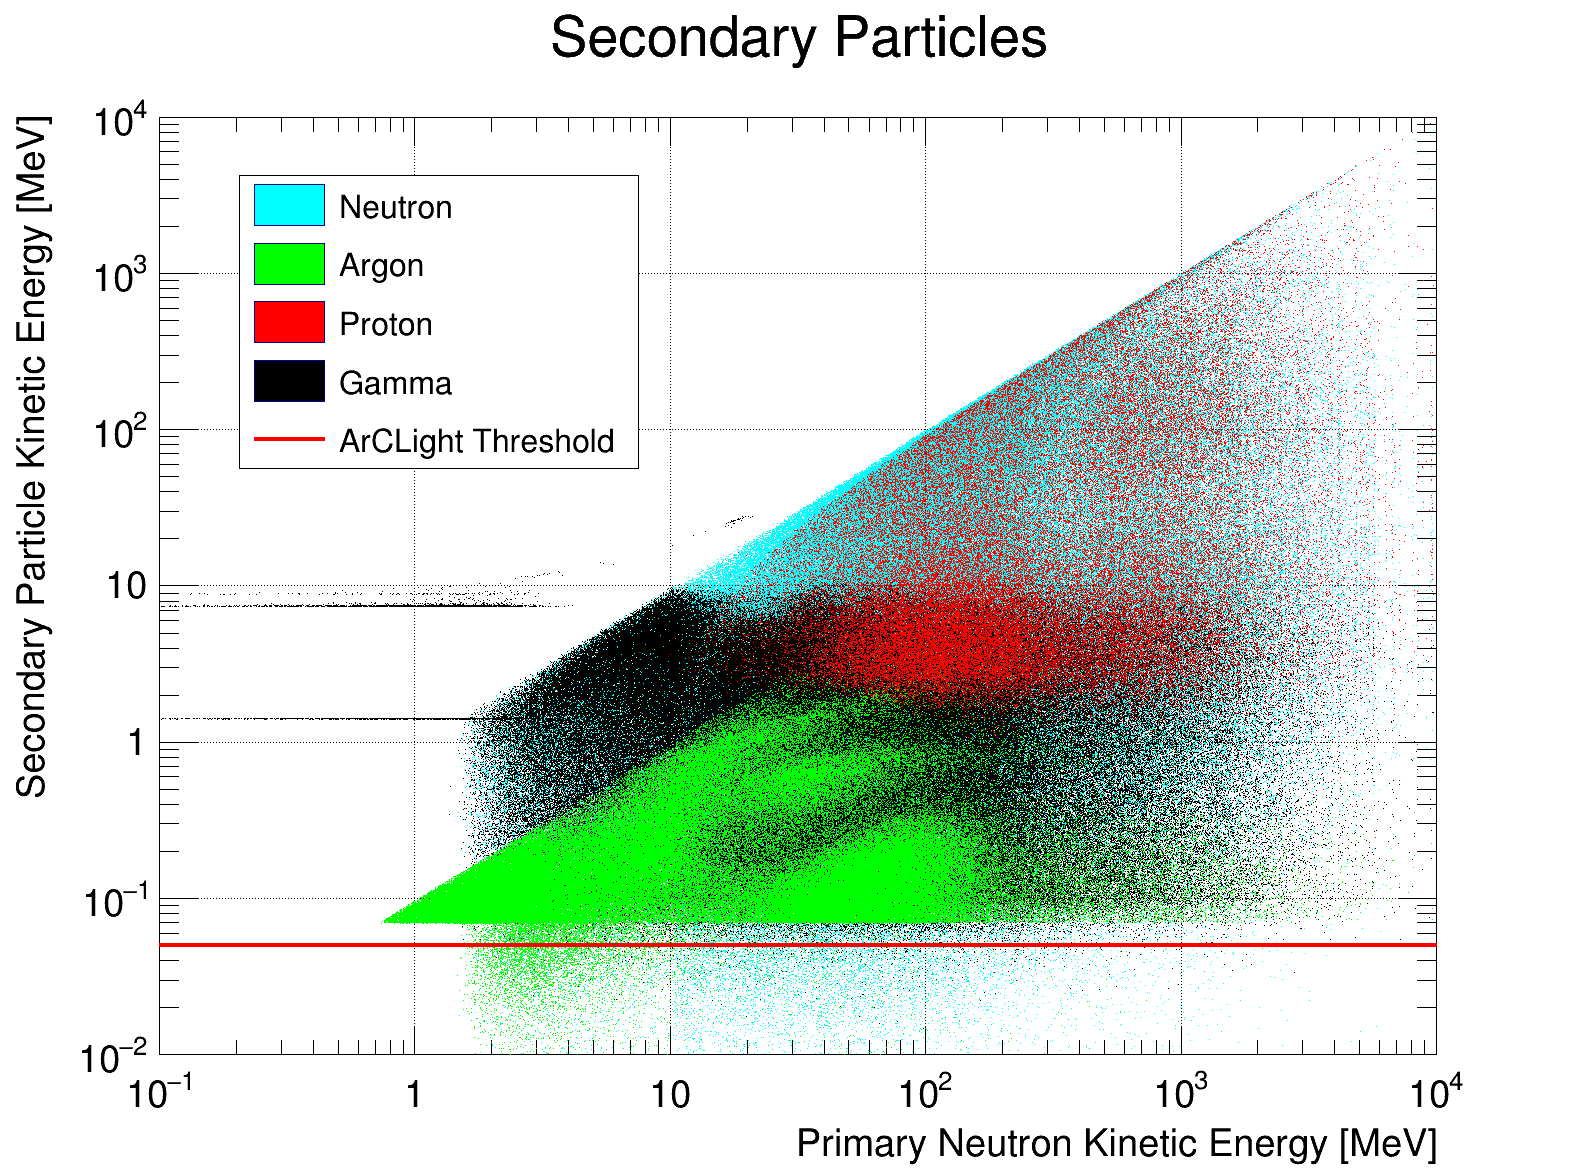
\includegraphics[width=0.8\textwidth]{plots/primary_neutron_recoils.png}
  \caption{Kinetic-energy distribution of secondary particles with respect to incident neutron kinetic energy for neutron interactions in LAr, shown for 100,000 simulated neutrino events (which may have more than one neutron produced at the vertex).}
  \label{fig:neutron_recoils}
\end{figure}
Figure~\ref{fig:neutron_recoils} shows the kinetic energy of secondary particles after the interaction of a primary neutron in LAr. The horizontal red line gives the energy threshold for the detection of these secondary particles with ArCLight~\cite{arclight}, assuming a conversion of 40k photons per MeV. Clearly, both recoiling argon nuclei and recoiling protons have kinetic energies well above the ArCLight detection threshold. While recoiling argon nuclei show typical energies between 100~keV and 1~MeV, recoiling protons show energies $>$~1~MeV, up to several GeVs.

\begin{figure}[htbp]
  \centering
  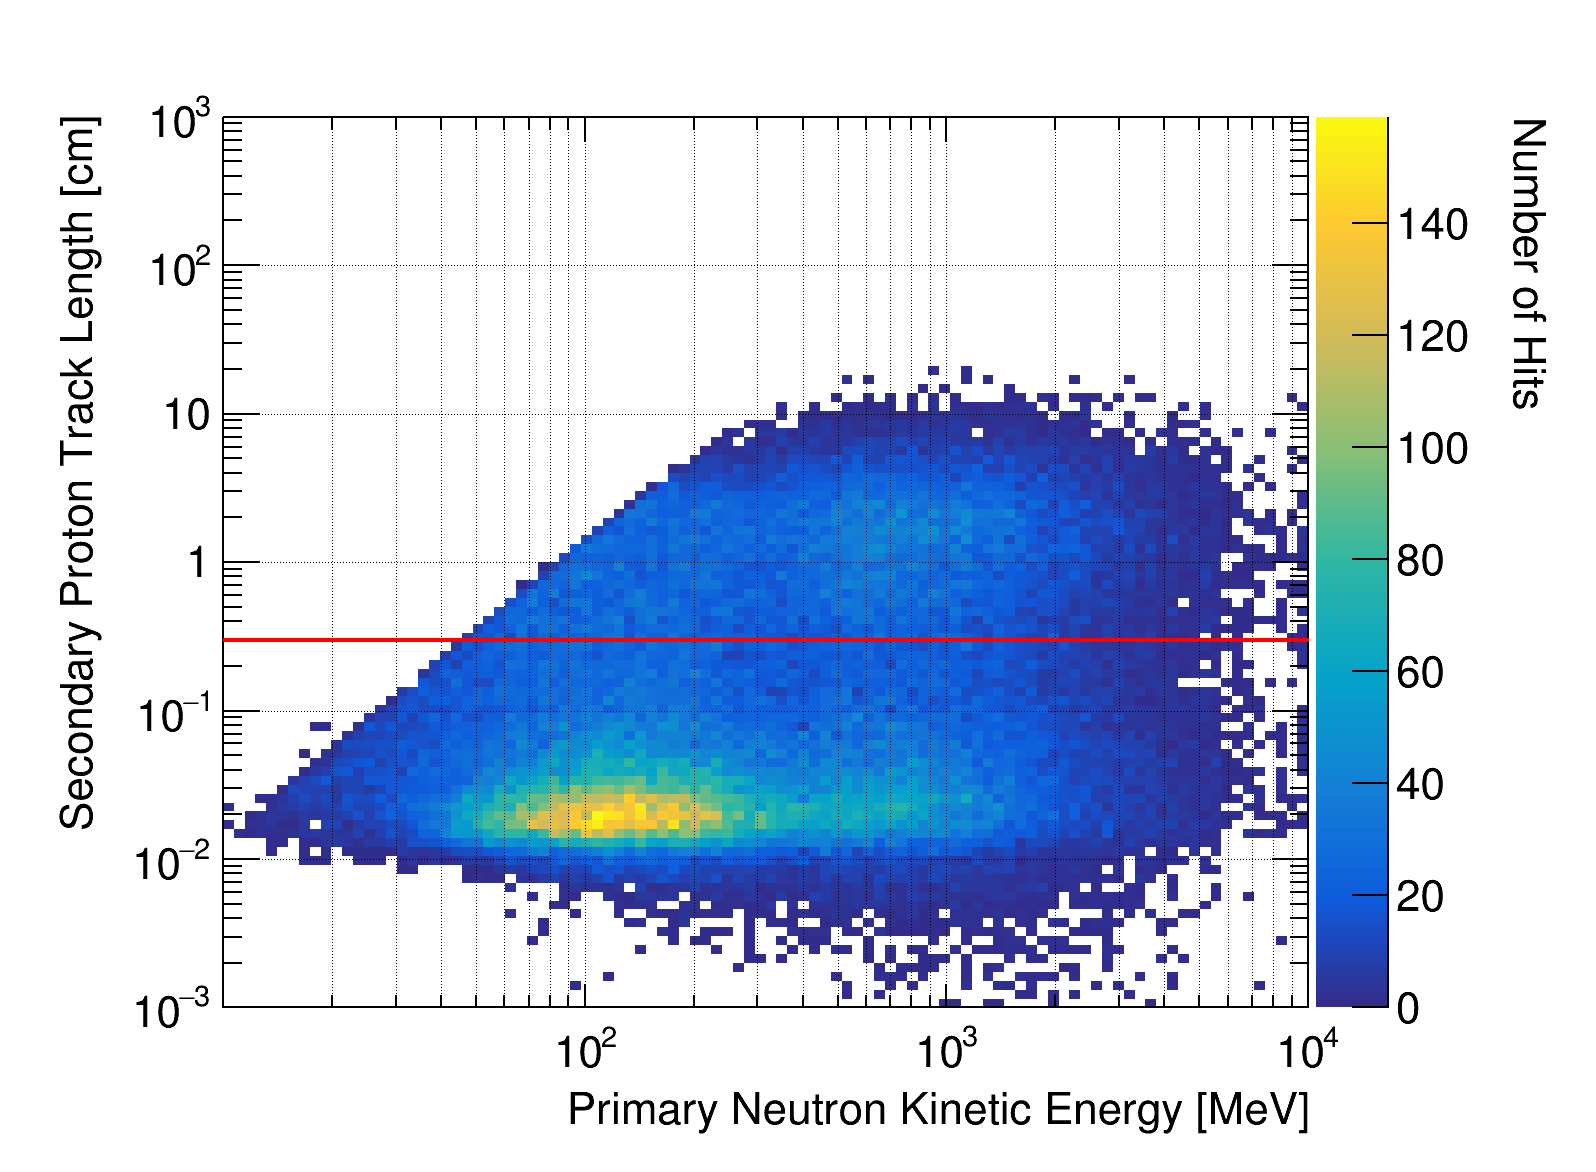
\includegraphics[width=0.8\textwidth]{plots/proton_track_length.png}
  \caption{Track length of recoiling protons for neutrons produced in 100,000 neutrino interactions. About 30\% of all recoils are resolvable as tracks with the LArPix pixel charge-readout system.The vast majority of neutron recoils contain no direction information, and will be detected only as single pixel hits.}
  \label{fig:proton_length}
\end{figure}

Given the LArPix $\sim$~3~mm pixel-pitch (see Section~\ref{sec:2x2-design}), the minimum reconstructable track length in ArgonCube is also $\gtrsim$~3~mm. Figure~\ref{fig:proton_length} shows the track length of recoiling protons with respect to the primary neutron kinetic energy. Recoiling protons can, depending on their energy, produce tracks which are up to $\sim$10~cm long. About 30~\% of all recoiling protons are resolvable by the pixelated charge readout, which correspond to protons that are knocked out of a nucleus by primary neutrons with energies $\gtrsim$~50~MeV.

\begin{figure}[htbp]
  \centering
  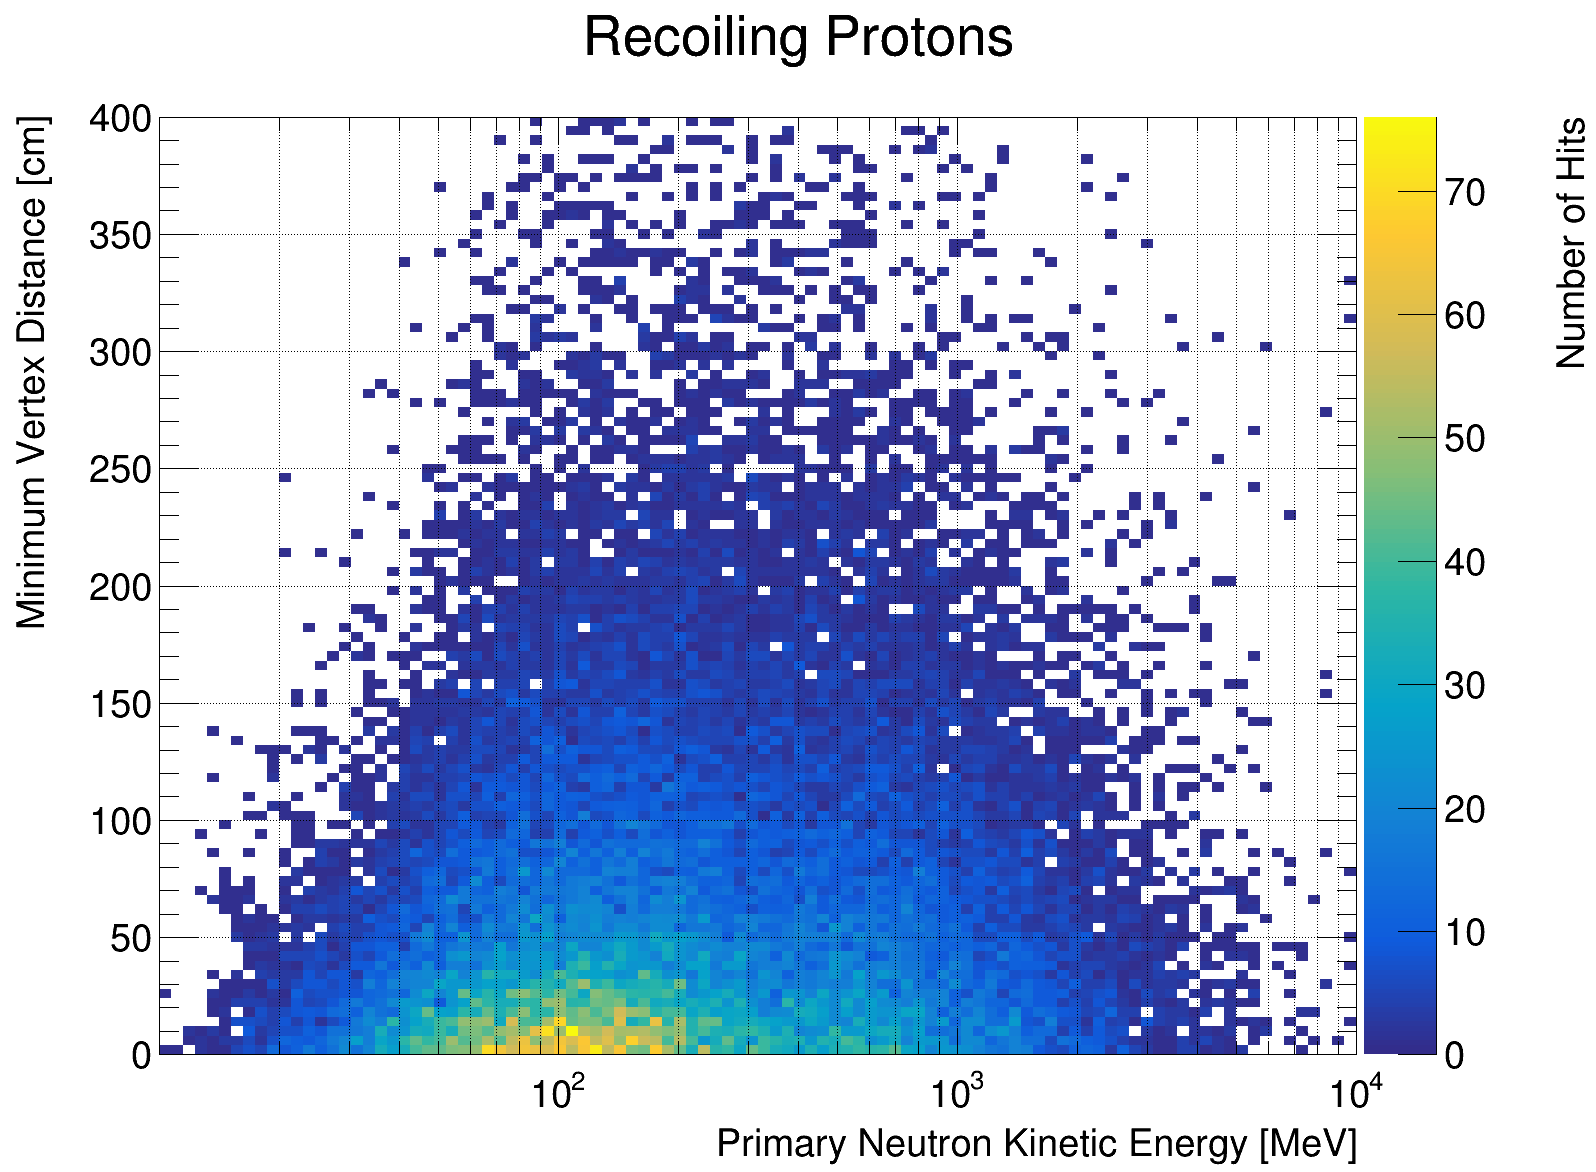
\includegraphics[width=0.8\textwidth]{plots/min_dist_vtx_proton_recoil.png}
  \caption{The minimum distance between the neutrino vertex and the neutron-induced proton track, as a function of neutron kinetic energy. Produced with 100,000 initial neutrino events simulated by ArgonBox.}
  \label{fig:min_dist_proton}
\end{figure}
Figure~\ref{fig:min_dist_proton} shows the minimum distance between the neutrino vertex and the neutron-induced proton track, as a function of neutron kinetic energy. The majority of proton recoils occur within 1 m, so many neutron-induced proton recoils will be contained within the 2x2 Demonstrator module.

%\FloatBarrier
\subsection{Reconstruction in a modular environment}
The module walls of the ArgonCube design produce gaps in particle tracks traversing multiple modules. This is not the same as dead wires in classic LArTPC readouts, as it results in only $\mathcal{O}\left(10\right)\,\mathrm{mm}$ gaps in energy deposits, rather than affecting sensitivity over large areas of charge readout. Algorithms to join such segmented tracks already exist~\cite{pandora}, but have not been adapted to the ArgonCube design. Simple track matching efficiencies across modules can be calculated using cosmics, which will be an essential first step. However, for events with many tracks produced at the vertex (see Figure~\ref{fig:track_multiplicity}), a detailed study of the reconstruction performance given the module walls will need to be carried out. ProtoDUNE-ND provides an opportunity to do so, and to check that the reconstruction behaves as expected, before moving to the full DUNE ND deployment of ArgonCube.

\begin{figure}[htb]
  \centering
  \subfloat[EM shower]       {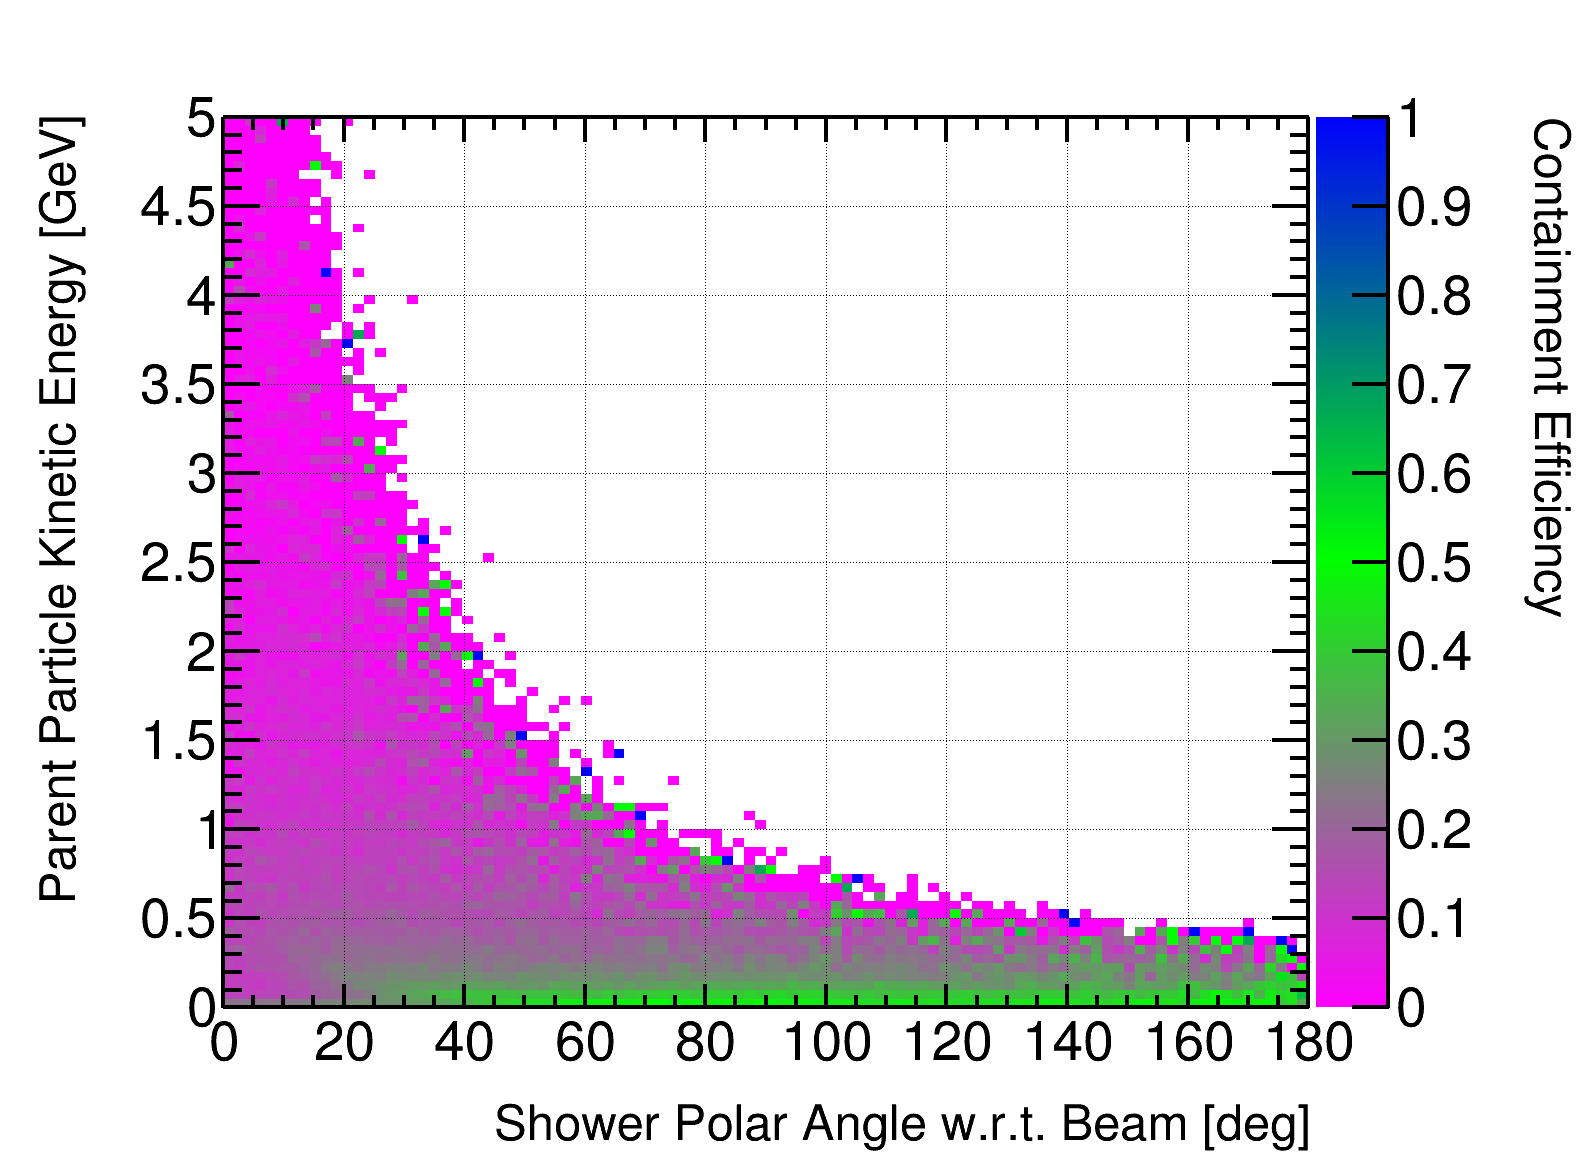
\includegraphics[width=0.5\textwidth]{plots/2x2_minerva_plots/EM_cont_eff_2x2.png}}
  \subfloat[Hadronic shower] {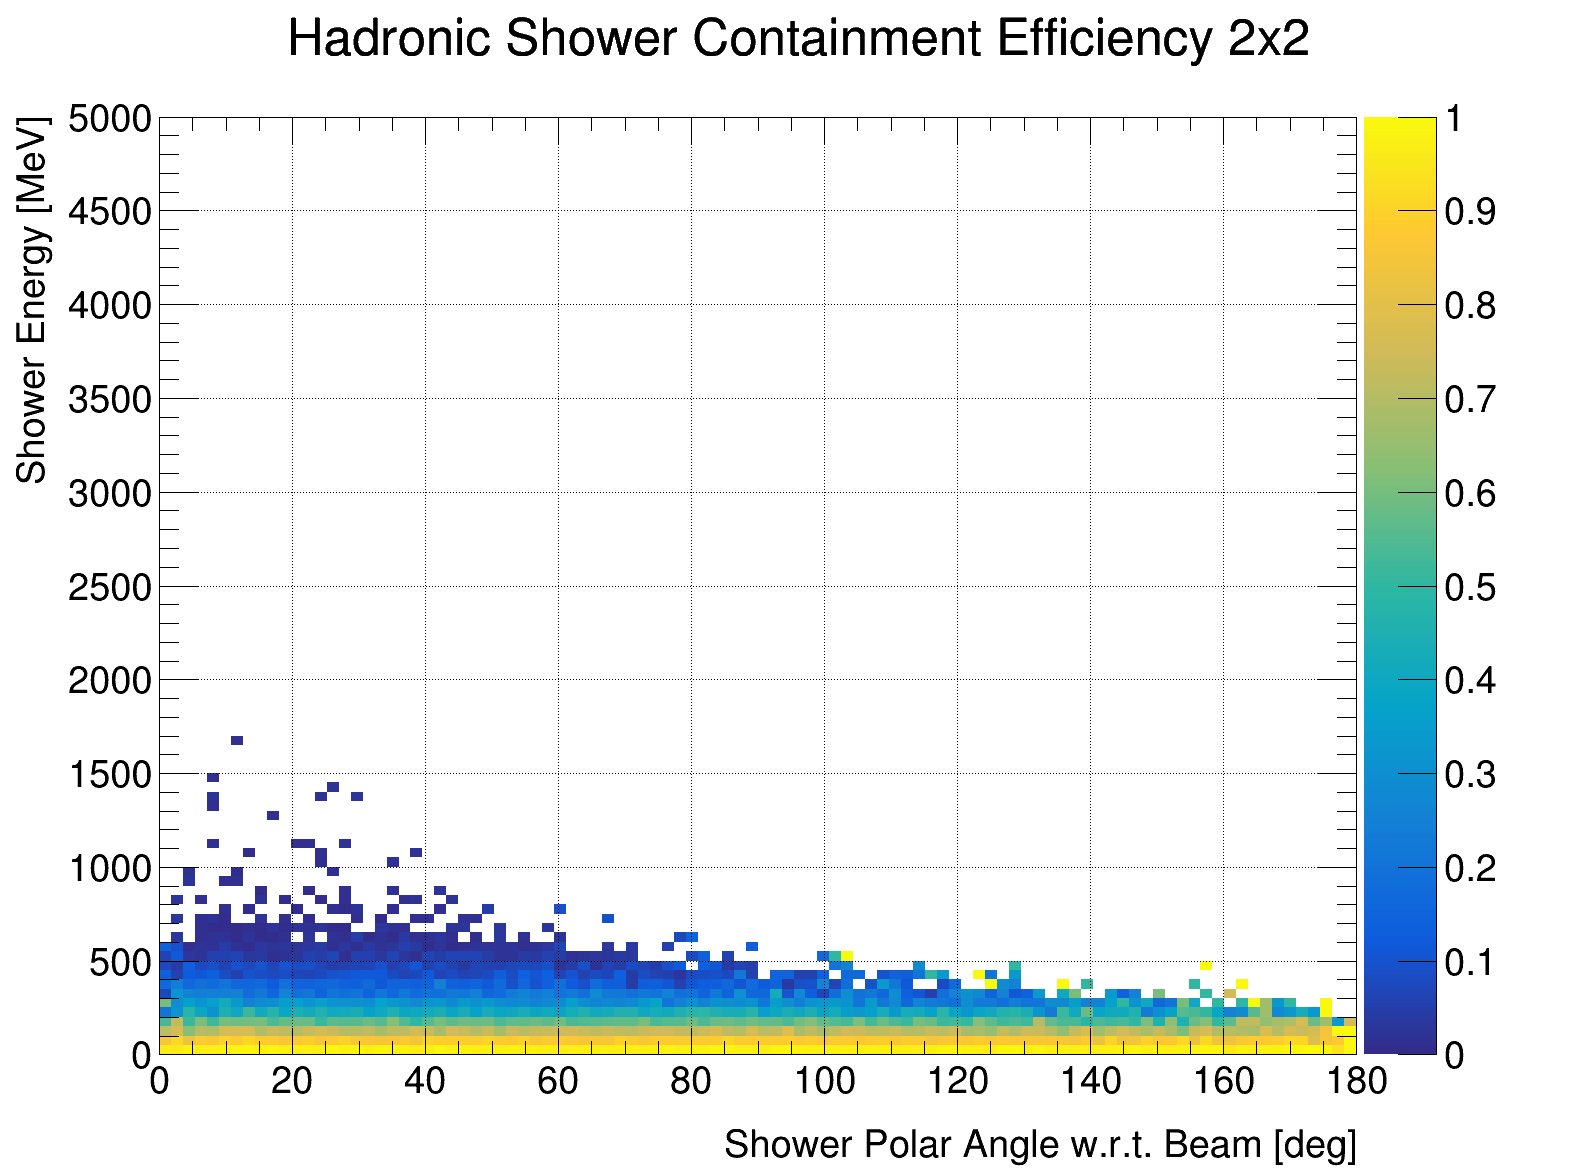
\includegraphics[width=0.5\textwidth]{plots/2x2_minerva_plots/H_cont_eff_2x2.png}}
  \caption{Containment efficiency for EM and hadronic showers produced by an interaction within the ArgonCube 2x2 active volume, as a function of initiator particle energy and angle w.r.t the incoming beam direction. Note that if $\geq 90$\% of energy is deposited within the 2x2 active volume, it is classed as contained.}
  \label{fig:2x2_shower_containment}
\end{figure}
This problem becomes significantly more complicated for electro-magnetic (EM), or hadronic, showers which cross modules. ProtoDUNE-ND will provide an opportunity to develop reconstruction software, and check how well it performs for realistic shower energies for neutrino interactions which cover the neutrino energy range of interest for the LBNF beamline. At these energies, shower development is known to be problematic, and shower reconstruction in LAr is a significant challenge. Additionally, in order to test how well the reconstruction can identify shower depth, a sample of fully contained showers would be extremely useful. Figure~\ref{fig:2x2_shower_containment} shows the efficiency to fully contain EM-showers or hadronic showers produced by an interaction within the ArgonCube 2x2 active volume, as a function of initiator particle energy and angle w.r.t the incoming beam direction. Note that if $\geq 90$\% of energy is deposited within the 2x2 active volume, it is classed as contained. 

\subsection{$\pi^{0}$ reconstruction}
A more quantitative measure of how well EM showers can be reconstructed in the modularized ArgonCube detector could be possible using $\pi^{0} \rightarrow \gamma\gamma$ decays (which have a branching ratio of 98.8\%~\cite{pdg_2018}), in which both decay photons produce a shower, and are contained in the active volume of the detector. Combining the information on the two showers, and attempting to reconstruct the invariant mass peak of the $\pi^{0}$ provides a measurement of the EM shower resolution. We note that Dalitz decay, $\pi^{0} \rightarrow \gamma e^{+} e^{-}$ (with a branching ratio of 1.2\%~\cite{pdg_2018}) may also be an interesting sample in such a high statistics environment, as only a single photon has to convert in the LAr. However, this sample was not considered further in this initial study.

\begin{figure}[htb]
  \centering
  \subfloat[$\pi^{0}$ multiplicity]   {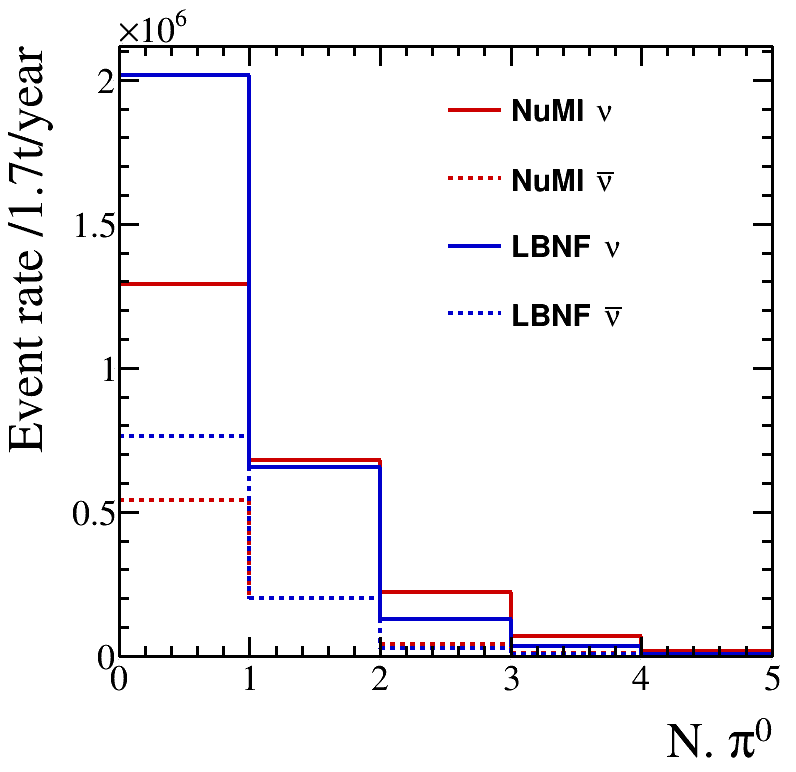
\includegraphics[width=0.5\textwidth]{plots/2x2_npi0_all.png}}
  \subfloat[$\pi^{0}$ momentum] {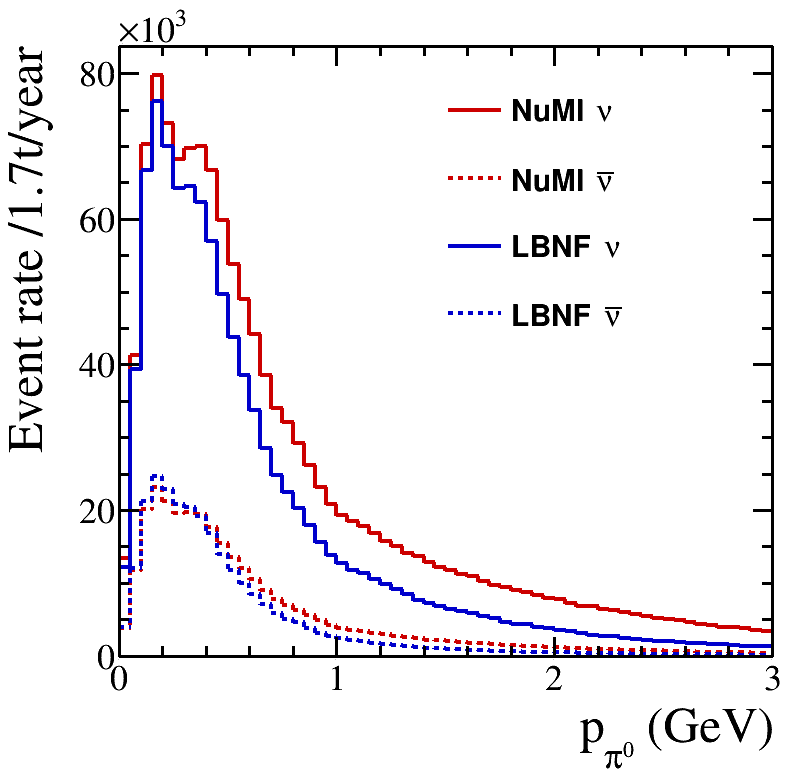
\includegraphics[width=0.5\textwidth]{plots/2x2_pi0_mom_all.png}}  
  \caption{The expected yearly rates of $\pi^{0}$'s produced at the vertex, as a function of event multiplicity and their momentum, expected in the 2x2 Demonstrator module's 1.7t LAr volume for the NuMI ME and LBNF fluxes, produced using GENIE v2.12.10 with the ``ValenciaQEBergerSehgalCOHRES'' configuration~\cite{genie}. Note that every $\pi^{0}$ from each event is included in the momentum distribution.}
  \label{fig:pi0_kinematics}
\end{figure}
Figure~\ref{fig:pi0_kinematics} shows the expected $\pi^{0}$ production rate in the active volume of the 2x2 Demonstrator module in the LBNF and NuMI ME beamlines, as a function of $\pi^{0}$ multiplicity in each event and $\pi^{0}$ momentum. There are, of course, some qualifiers for this study. Many photon-induced showers will not be contained, and those which are will be lower energy than many EM showers expected in the DUNE ND. Figure~\ref{fig:pi0_containment_2x2} shows the efficiency for containing both photon-induced showers from a primary $\pi^{0}$ decay in the ArgonCube 2x2's active volume, shown for all $\pi^{0}$'s produced inside that volume. As expected, the efficiency is low for high energy pions, but it will still be possible to reconstruct a large fraction of the lower momentum $\pi^{0}$'s from Figure~\ref{fig:pi0_kinematics}. Overall, this study shows that this $\pi^{0}$ mass peak reconstruction will be a worthwhile study at ProtoDUNE-ND.

\begin{figure}[htb]
  \centering
  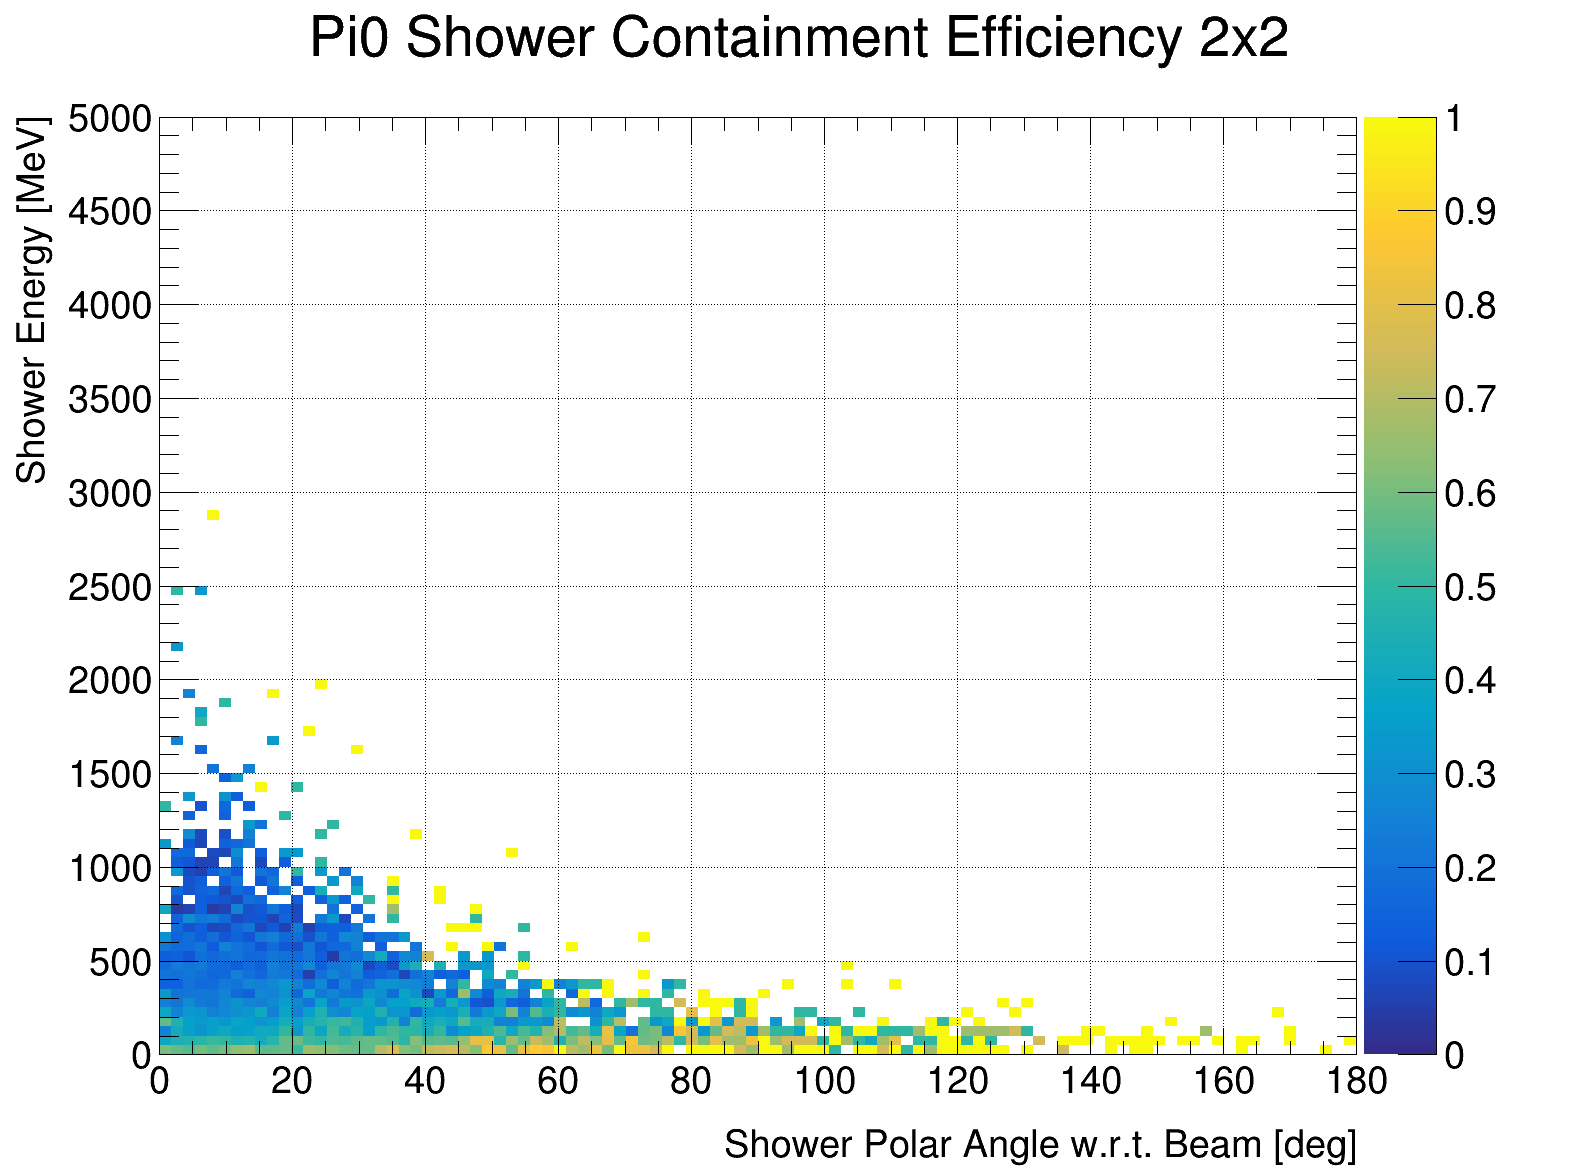
\includegraphics[width=0.5\textwidth]{plots/2x2_minerva_plots/Pi0_cont_eff_2x2.png}
  \caption{Efficiency for containing both photon-induced showers from $\pi^{0}$ decays in the ArgonCube 2x2 module, as a function of the $\pi^{0}$ kinetic energy and angle w.r.t the incoming neutrino direction. Containment is defined as $\geq$90\% of the energy being deposited in an active volume of a detector, and all primary $\pi^{0}$'s produced inside the 2x2's active volume are included.}
  \label{fig:pi0_containment_2x2}
\end{figure}
Two further issues for this study are apparent. Firstly, events with more than one $\pi^{0}$ introduce a problem: even if two EM showers are fully contained, they may not come from the same $\pi^{0}$ decay. Secondly, of those $\pi^{0}$ decays for which both photons are fully contained, the initial $\pi^{0}$ is likely to have a low momentum, which is likely to exclude some fraction of the higher invariant mass events. However, despite these challenges, a measure of EM shower resolution from ProtoDUNE-ND would be very useful for DUNE ND design studies, so this possibility is worth investigating further.

Studies have shown that a 3D-charge readout will improve reconstruction of $\pi^{0}$ showers by removing energy deposits from events crossing the shower~\cite{Damian}. However, as for any LArTPC a first step for the 2x2 will be to demonstrate electron-photon separation near the vertex.    

%\FloatBarrier
\subsection{Space charge and electric field uniformity}
\label{sec:efield}
A concern for LAr detectors in a high intensity beam is the build up of space charge --- long-lived argon ions which drift slowly towards the cathode --- and possible affects on the uniformity of the electric field which may accumulate over time. In currently operating and near-future LAr detectors~\cite{Ereditato:2014lra, Antonello:2015lea}, both cosmic tracks and UV lasers are used to calibrate for distortions in the electric field. Both the UV laser track and high energy cosmic muons are expected to leave straight tracks in the detector. If the drift field is not uniform across the detector, ionization electrons produced along the length of this track will not drift at the same speed, or with a constant direction, and will result in a distorted track at the readout plane. By comparing the reconstructed and expected track, a map of the electric field distortion can be built up for calibration purposes.

Assuming that the 2x2 Demonstrator module is equipped with scintillator panels to tag cosmic tracks using a timing coincidence between two sides of the detector, and reasonable spatial resolution on those scintillator paddles, electric field distortions could be measured in the 2x2 Demonstrator module. By looking at beam-on, and beam-off data, it would be possible to look at the possible affect of space charge build-up over time due to the high event rate in the NuMI beam. If significant space charge build-up were observed, this would inform the future ArgonCube design for the DUNE ND, as a higher drift field strength would be required.

Additionally, although the electric-field uniformity of the resistive field shell will be checked in a small scale LAr TPC at Bern, a check of the electric-field uniformity and stability over time for full-size ArgonCube modules would be a valuable final validation of the design.

\subsection{Cosmic and Rock Muon suppression}
\label{sec:cosmic-suppression}

The DUNE ND is located underground with a \SI{50}{\metre} overburden, that reduces the cosmic flux by orders of magnitude compared to surface detectors. The cosmic rate in MINERvA is \SI{18}{\hertz}, for $\sim$\SI{6}{\metre\squared}.  For the ArgonCube 2x2, the $\sim$\SI{150}{\micro\second} readout window, assuming $\sim$\SI{2}{\metre\squared}, the rate of cosmics muons is 0.001 per readout window. Reading out around spills only, will result in a coincident cosmic muon once every 20 minutes.
In DUNE ND we expect $\sim$10 rock muons per spill, which will be on average $\sim$\SI{1}{\micro\second} apart in time. They are unlikely to overlap any neutrino activity in 3D, but the fast timing will provide an additional handle.
A key design choice for the DUNE ND is whether or not a muon tagging system is required --- for example, a series of scintillator planes surrounding the LAr TPC, as for SBND and MicroBooNE~\cite{CRT}. The proposed ProtoDUNE-ND test experiment can help inform this design choice, assuming that the ArgonCube 2x2 Demonstrator module is equipped with scintillator paddles.

By using the scintillator paddles to tag cosmic or rock events using a timing coincidence, methods for rejecting them can be validated independently. For example, we expect that the good timing resolution and light localization from ArcLight will allow cosmics out of the beam window to be rejected with a high efficiency. Additionally, if a cosmic muon traverses a pixel plane, or an ArcLight plane, we would expect to see a large charge deposition or a large number of photoelectrons measured, which could be an additional way to reject cosmic muons. Both of these methods can be validated with ProtoDUNE-ND.

\subsection{Reconstruction with multiple subdetectors}
Because the ArgonCube 2x2 Demonstrator module is relatively small, many events from the NuMI ME beam will not be contained. Figure~\ref{fig:leaky_event} shows a neutral current event where many pions are produced, but in which the pions and subsequent hadronic showers extend far beyond the detector. Such events are likely to be uncontained even in the full ArgonCube component of the DUNE ND. In charged-current events, the muon will be uncontained most of the time. For this reason, and because it is not possible to magnetize the large LAr component, a magnetized tracking detector is proposed downstream of ArgonCube in the DUNE ND. A test module for the HPTPC is hoped to be included as part of the ProtoDUNE-ND effort as described in Section~\ref{sec:tracking_detectors}. With multiple subdetectors included in ProtoDUNE-ND, multi-detector reconstruction capabilities can be developed and tested. Additionally, if the sign and momentum of escaping hadrons and muons can be measured, it may be possible to make physics measurements with ProtoDUNE-ND, which would be beneficial to the overall DUNE program. For that reason, if no downstream tracker is available, it would be highly desirable to utilize the proximity of the MINERvA and MINOS-ND detectors, and try to minimize the distance between the ArgonCube 2x2 Demonstrator module and those detectors, in order to use them as downstream trackers.
\begin{figure}[htb]
  \centering
  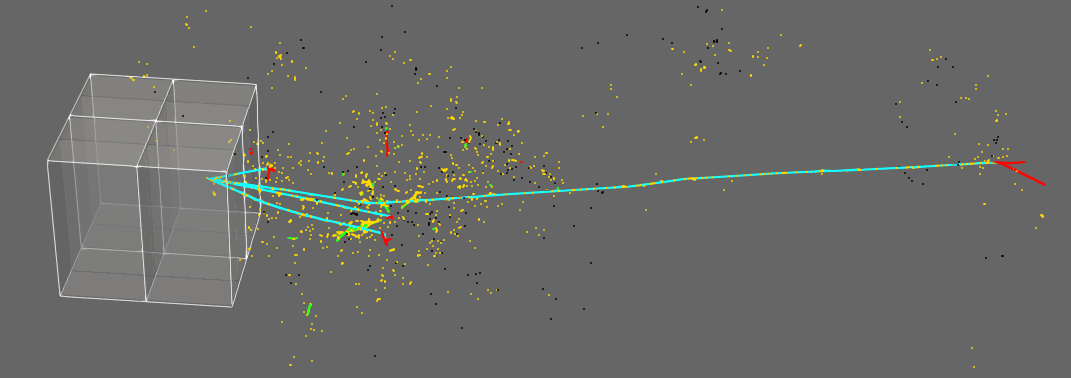
\includegraphics[width=0.8\textwidth]{{plots/EventDisplays/8.17GeV_rectangle_crop}.png}
  \caption{Example ArgonBox simulated event for an 8.17 GeV $\nu_{\mu}$--argon neutral-current multi-pion interaction, in which the pions are not contained in the module. Energy deposits in a bulk volume of LAr are color-coded according to the particle type: $\pi^{\pm}$ --- blue; $\mu^{\pm}$ --- purple; $e^{+}$ --- green; $e^{-}$ --- yellow; proton --- red; recoiling nuclei --- black. The event vertex was randomly placed inside the active volume of the 2x2 Demonstrator module, the geometry for which is superimposed on these images, but which is not simulated by ArgonBox.}
  \label{fig:leaky_event}
\end{figure}
\FloatBarrier

\section{Incorporating other detector prototypes into ProtoDUNE-ND}
\label{sec:MINERvA_MINOS}

\begin{figure}[htb]
	\centering
	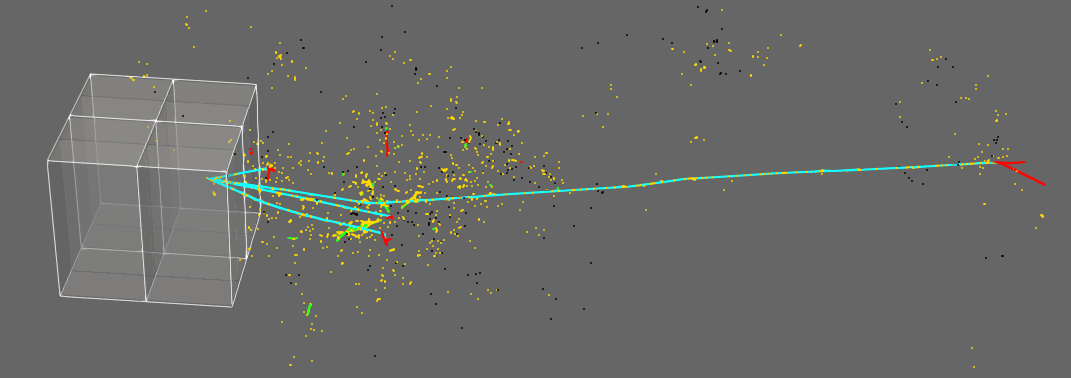
\includegraphics[width=0.8\textwidth]{{plots/EventDisplays/8.17GeV_rectangle_crop}.png}
	\caption{Example ArgonBox simulated event for an 8.17 GeV $\nu_{\mu}$--argon neutral-current multi-pion interaction, in which the pions are not contained in the module. Energy deposits in a bulk volume of LAr are color-coded according to the particle type: $\pi^{\pm}$ --- blue; $\mu^{\pm}$ --- purple; $e^{+}$ --- green; $e^{-}$ --- yellow; proton --- red; recoiling nuclei --- black. The event vertex was randomly placed inside the active volume of the ArgonCube 2x2 Demonstrator, the geometry for which is superimposed on these images, but which is not simulated by ArgonBox.}
	\label{fig:leaky_event}
\end{figure}
Given the ArgonCube 2x2 Demonstrator's size and the relatively high energy NuMI ME beam, many events will not be contained in the 2x2 alone. Figure~\ref{fig:leaky_event} shows a neutral current event where many pions are produced, but in which the pions and subsequent hadronic showers extend far beyond the detector. Indeed, many such events would not be contained in the full ArgoNCube deployment at the DUNE ND, in the LBNF beamline, and for charged-current events, the muon will be uncontained most of the time. For this reason, and because it is not possible to magnetize the large LAr component, further, magnetized, tracking detectors are proposed downstream of ArgonCube in the full DUNE ND complex, and the requirement to tag side-escaping particles is discussed in Ref.~\cite{dune_ndcsg}. Broadly speaking, three additional subdetector options are considered for the DUNE-ND design, in addition to ArgonCube~\cite{dune_ndcsg}, as introduced in Section~\ref{sec:tracking_detectors}: a scintillator tracking detector; a magnetized low-density tracking detector; and a Cosmic Ray Tagging (CRT) system.

Prototypes for these detectors are also being planned, and the ProtoDUNE-ND complex is intended to evolve over time to accommodate them. As has been remarked, the cryogenic system for the ArgonCube 2x2 will be moveable to test key components of the DUNE-PRISM technical design, which will allow ProtoDUNE-ND to be easily reconfigured to accommodate any future prototype detectors. In this section, we discuss how adding those additional detectors will enhance the neutrino engineering studies possible with the ArgonCube 2x2 Demonstrator alone. With multiple subdetectors included in ProtoDUNE-ND, multi-detector reconstruction capabilities can be developed and tested. Additionally, if the sign and momentum of escaping hadrons and muons can be measured, it may be possible to make physics measurements with ProtoDUNE-ND, which would be beneficial to the overall DUNE program.

\subsection{Scintillator tracking detector}
\label{sec:minerva}
Two distinct scintillator options are currently being considered for the DUNE ND design, as introduced in Section~\ref{sec:tracking_detectors}. A large, fully active, Three-Dimensional Scintillator Tracker (3DST), and scintillator components downstream of the HPgTPC to tag escaping neutral particles. %As discussed in Section~\ref{sec:detector-physics-studies}, a large fraction of particles will not be contained in the 2x2 alone. A downstream scintillator detector would recover many of these particles, and would make it possible to benchmark the 2x2 response to a wider range of particle energies, and therefore the expected DUNE phase-space.

To investigate the effect that adding a scintillator component, and generically a downstream tracking detector, to ProtoDUNE-ND, a simulation was performed where a generic scintillator box was included downstream of the ArgonCube 2x2 Demonstrator. Neutrino interactions are generated in the ArgonCube active volume, and propagated through an approximation of the ArgonCube 2x2 demonstrator and scintillator block.  The scintillator detector used is simply a rectangular box, \SI[product-units=repeat]{1.4x1.4}{\metre\squared} in the dimensions transverse to the beam, making it large enough to cover the downstream face of the 2x2 active volume. In the beam direction, the scintillator is split into 

, and~\todo{how long?}  The simulation includes the most downstream 12 modules (24 planes) of the tracker region, as well as the full downstream ECAL and HCAL regions.  The rectangular box represents the central part of the MINERvA inner detector, and is large enough to cover the entire ArgonCube active volume. An example event is shown in Figure~\ref{fig:2x2+MINERvA_event}, and can be compared with 2x2 only events in Figures~\ref{fig:argonbox_event_display} and~\ref{fig:leaky_event}. Note that this simulation only included the ArgonCube cryostat and MINERvA detector components, no material was included outside these (so escaping particles simply leave without ever re-interacting). This is unlike the previously described ArgonBox simulation, where a large box of argon was simulated (so escaping particles still re-interact). Events were again distributed uniformly throughout the ArgonCube active volume.
\begin{figure}[htb]
  \centering
  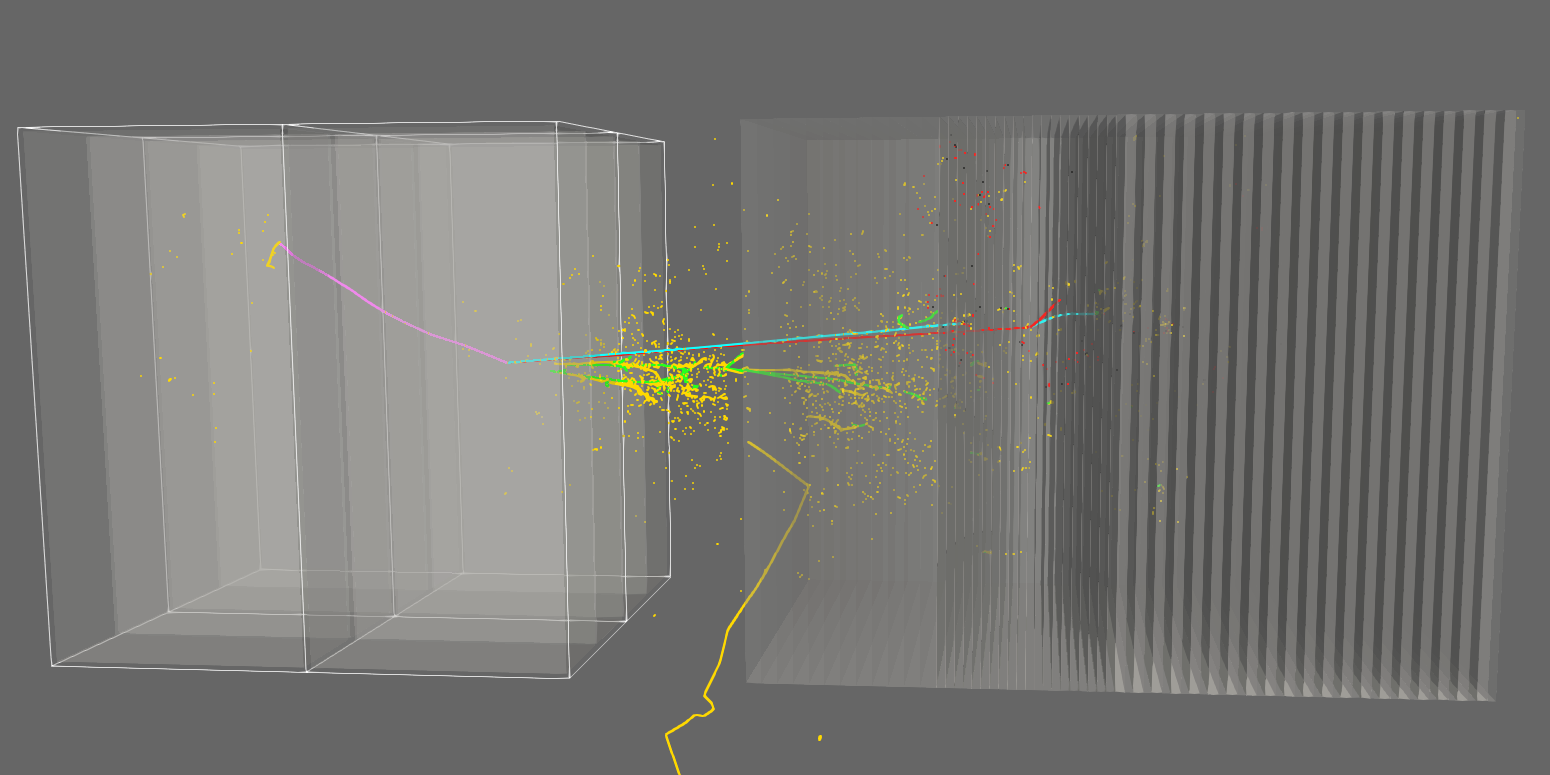
\includegraphics[width=0.8\textwidth]{{plots/Event_Displays_2x2_MINERvA/MINERvA_full_e70_rectangle_crop}.png}
  \caption{Example simulated event for a 7.0 GeV $\nu_{\mu}$--argon charged-current interaction, in which particles not contained in the ArgonCube 2x2 enter the scintillator block detector. Energy deposits are color-coded according to the particle type: $\pi^{\pm}$ --- blue; $\mu^{\pm}$ --- purple; $e^{+}$ --- green; $e^{-}$ --- yellow; proton --- red; recoiling nuclei --- black. The event vertex was randomly placed inside the active volume of the 2x2 Demonstrator module.}
  \label{fig:2x2+MINERvA_event}
\end{figure}

In the following, we discuss potential detector physics studies, or improvements to detector physics studies previously discussed in the ArgonCube 2x2-only case (in Section~\ref{sec:detector-physics-studies}), incorporating elements of the MINERvA detector downstream of the ArgonCube 2x2 module.

\subsubsection{Track matching}
All DUNE ND designs considered in Ref.~\cite{dune_ndcsg} include some fast scintillator component, downstream of the LAr ArgonCube component, and downstream of a low-density GAr TPC tracker, to tag escaping particles, photons, and possibly neutrons. There is a significant reconstruction challenge in matching the escaping tracks from the LAr component, with the signals in the scintillator, given the slow charge readout in the LAr TPC, and the high multiplicity DUNE-ND environment.

\begin{figure}[htb]
  \centering
  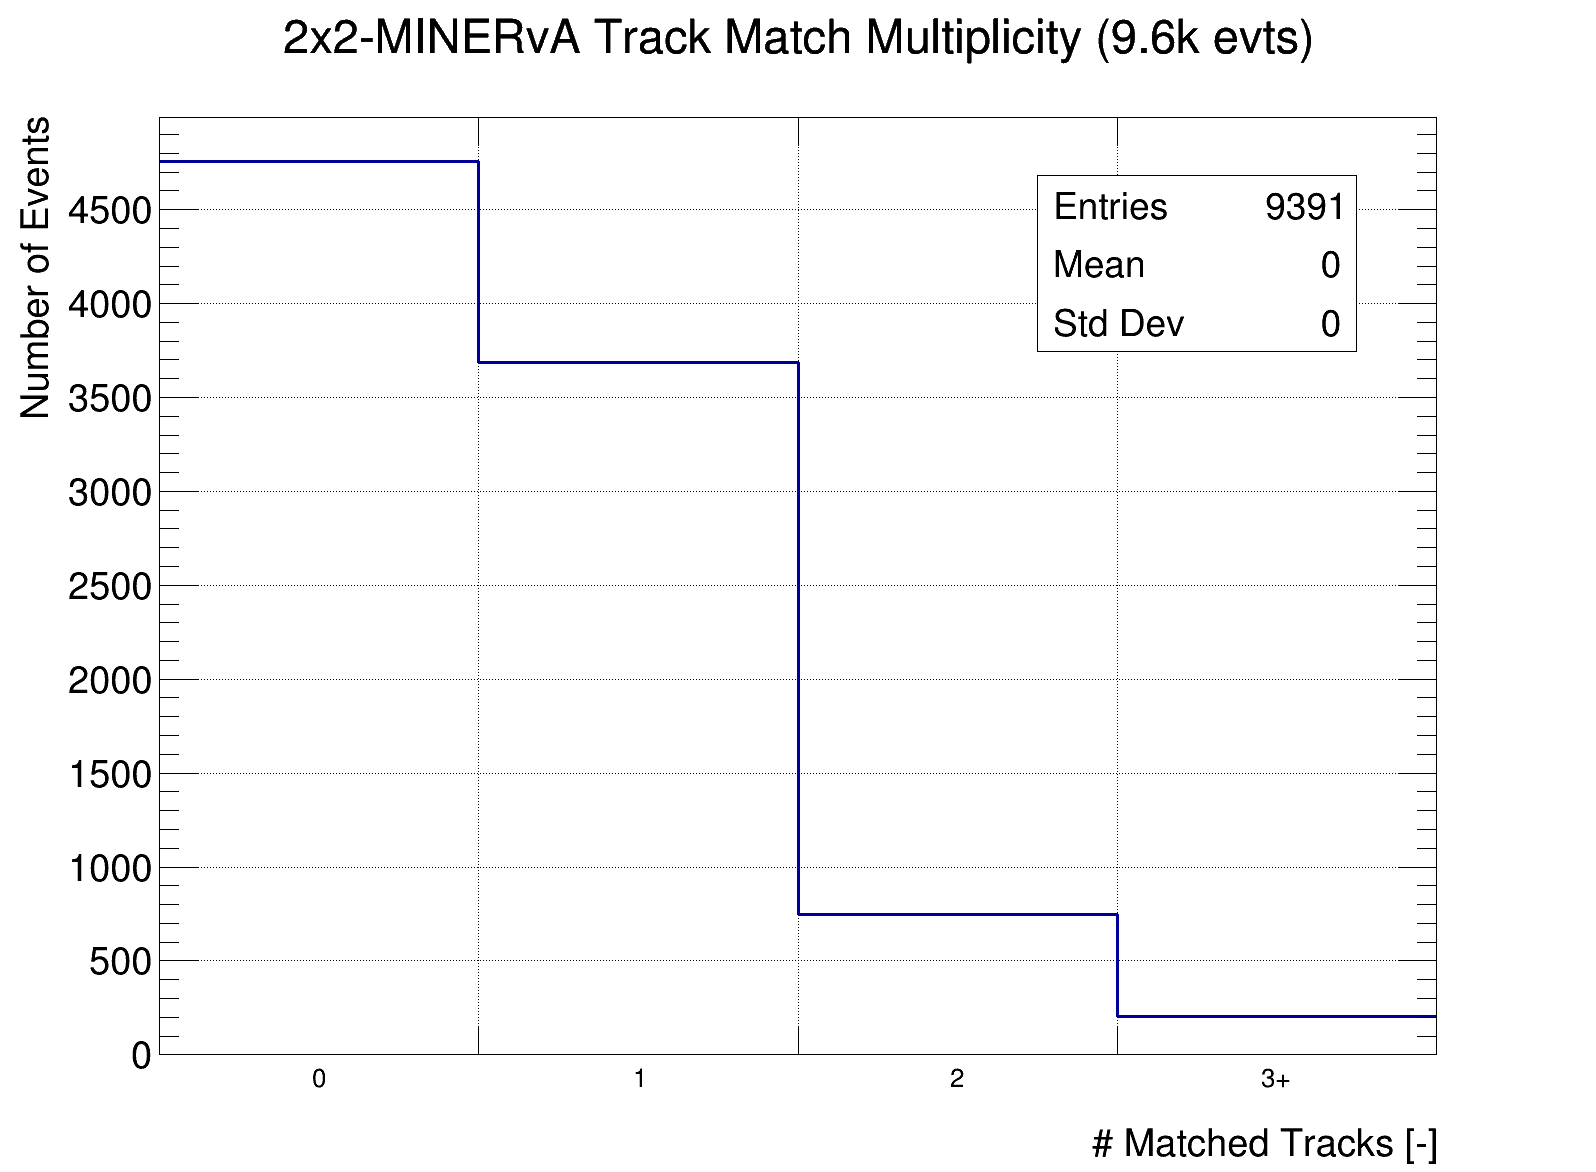
\includegraphics[width=0.6\textwidth]{plots/2x2_minerva_plots/track_mathch_multiplicity.png}
  \caption{Simulated number of true tracks produced by simulated GENIE interactions in the ArgonCube 2x2 active volume, which deposit energy in both the 2x2 module, and the MINERvA component positioned downstream of the 2x2.}
  \label{fig:track_multiplicity_min}
\end{figure}
Many tracks produced in the LAr volume are not contained by the ArgonCube 2x2 module, and the majority will escape downstream. In Figure~\ref{fig:hadronic_containment}, the multiplicity of tracks which deposit charge in both the ArgonCube 2x2 module and the MINERvA component, included in the simulation described above, are shown. Full DUNE-ND events are likely to have an even higher LAr to scintillator track multiplicity due to the pile-up in the much larger 35 t ArgonCube LAr detector. But it is clear from Figure~\ref{fig:track_multiplicity_min} that including MINERvA elements in the ProtoDUNE-ND tests would provide useful data with which to start tackling this reconstruction problem.

\begin{figure}[htb]
  \centering
  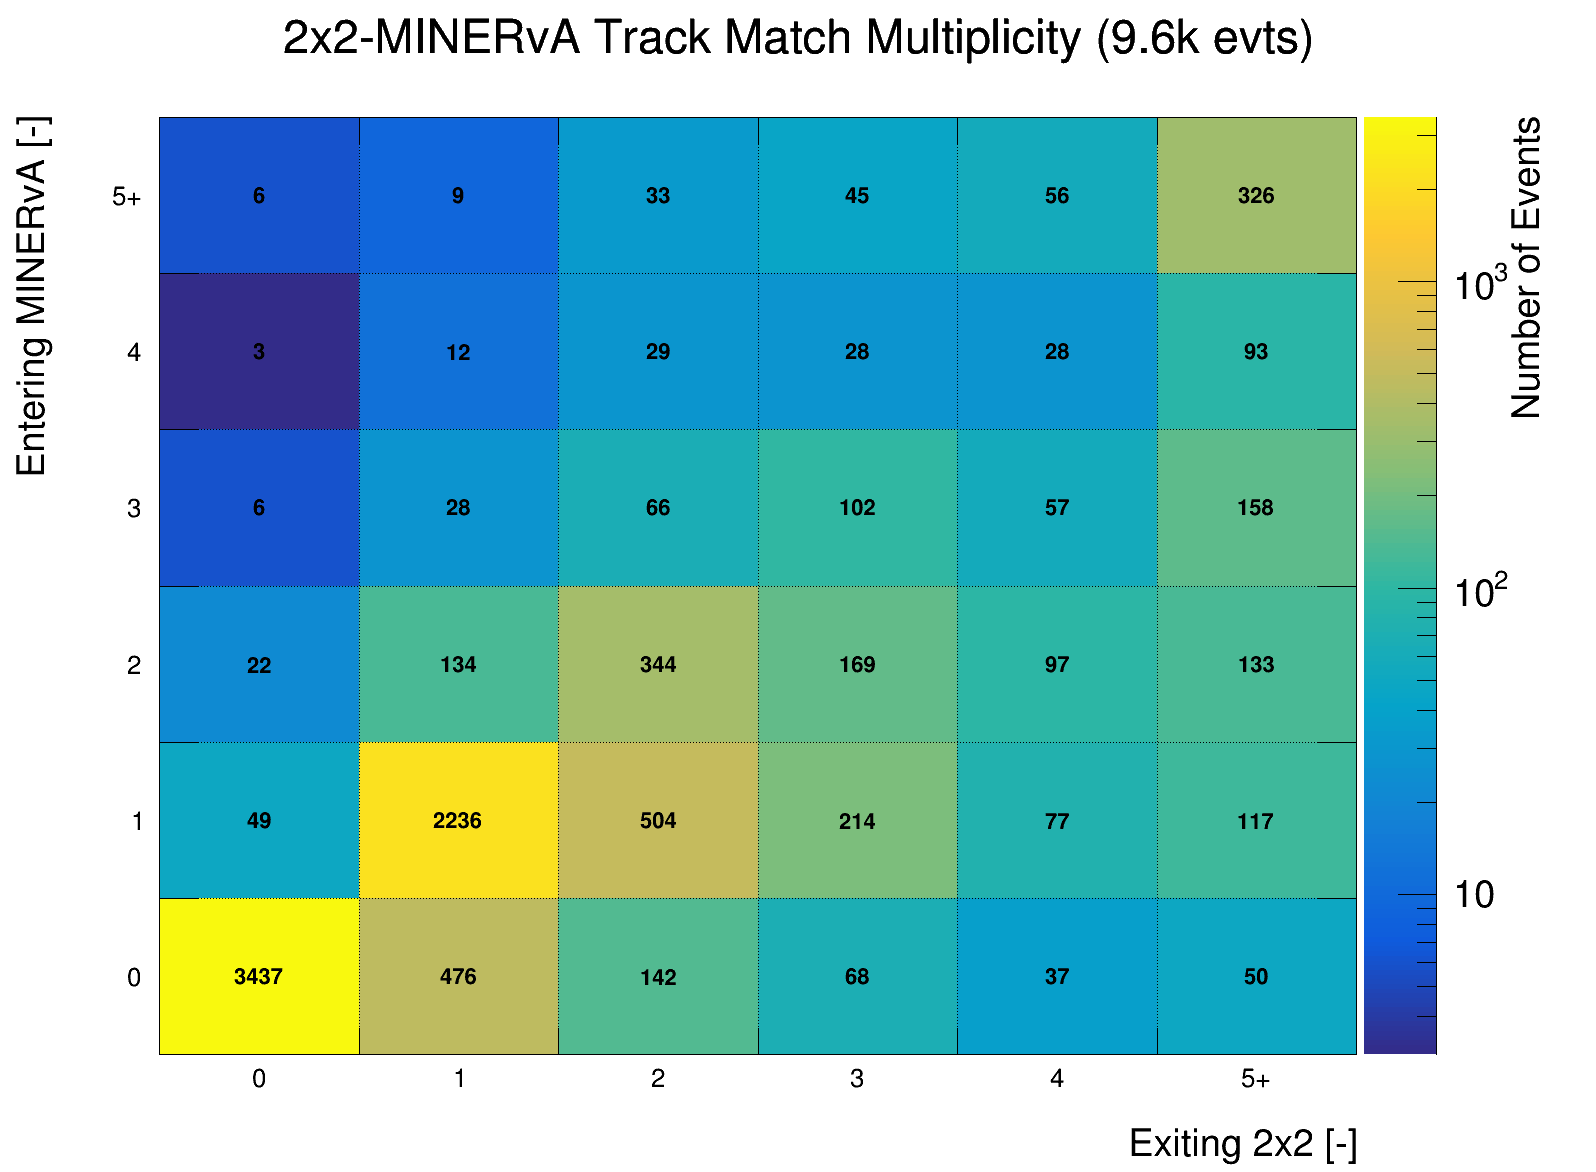
\includegraphics[width=0.6\textwidth]{plots/2x2_minerva_plots/track_mathch_topo.png}
  \caption{Simulated number of true tracks produced by simulated GENIE interactions in the ArgonCube 2x2 active volume, which exit the downstream face of the 2x2 module, relative to the number of tracks which enter the upstream face of the downstream MINERvA component, event by event.}
  \label{fig:track_multiplicity_topo}
\end{figure}
As can be seen from the event display shown in Figure~\ref{fig:2x2+MINERvA_event}, events in which tracks escaping the 2x2 active volume may re-interact in the surrounding LAr bath before entering the MINERvA component included in this simulation, thus making the event more confusing, and difficult to assess reconstruction performance with. Figure~\ref{fig:track_multiplicity_topo} shows the multiplicity of tracks exiting the downstream face of the 2x2 active volume downstream, compared with the number of tracks entering the upstream face of the MINERvA component included in the simulation. The distribution is fairly diagonal, suggesting that although complicated event topologies exist, the events will not be too confused to use for these studies. Note also that this problem could be dramatically reduced by partially instrumenting the dead region between the two detectors.

\subsubsection{Acceptance studies}
\label{sec:minerva-acceptance}
The inclusion of MINERvA in ProtoDUNE-ND will improve the acceptance of particles for various studies. Here, we show how the efficiency for contained events compares for the 2x2+MINERvA setup desribed above, with MINERvA components located downstream of the ArgonCube 2x2 Demonstrator module, and for the 2x2-only case.

\begin{figure}[htb]
  \centering
  \subfloat[2x2-only]    {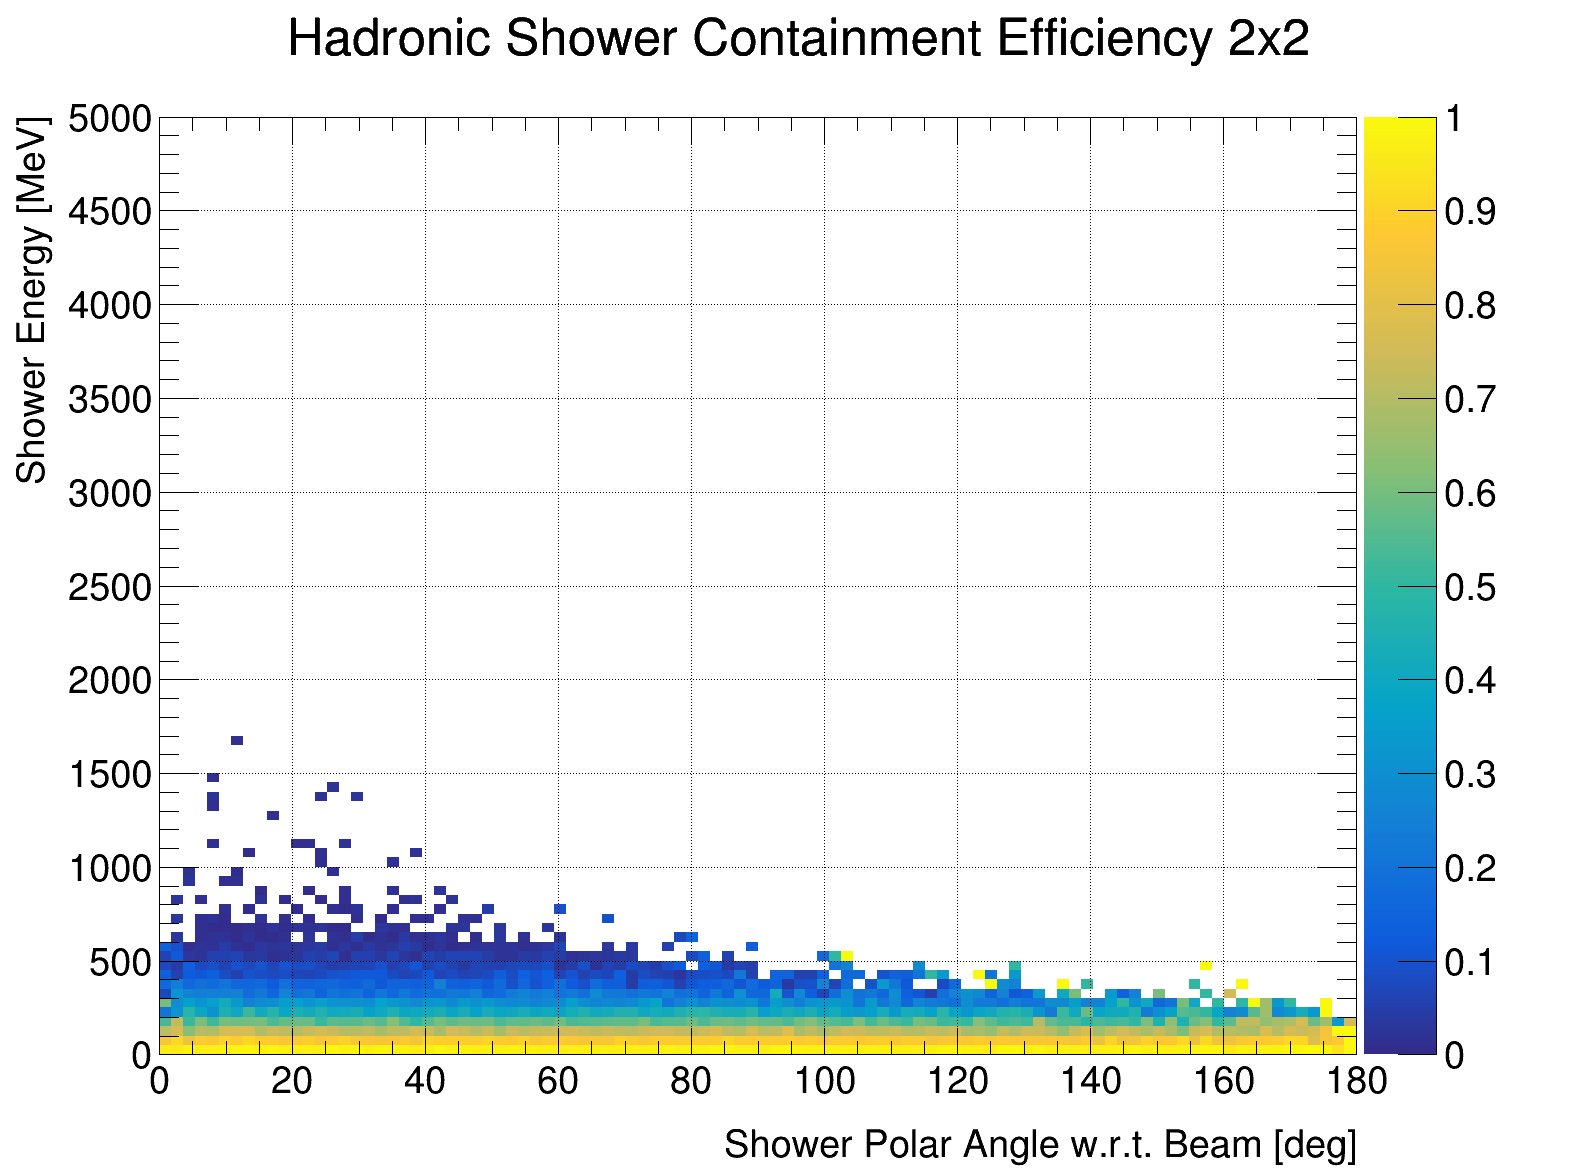
\includegraphics[width=0.45\textwidth]{plots/2x2_minerva_plots/H_cont_eff_2x2.png}}
  \subfloat[2x2+MINERvA] {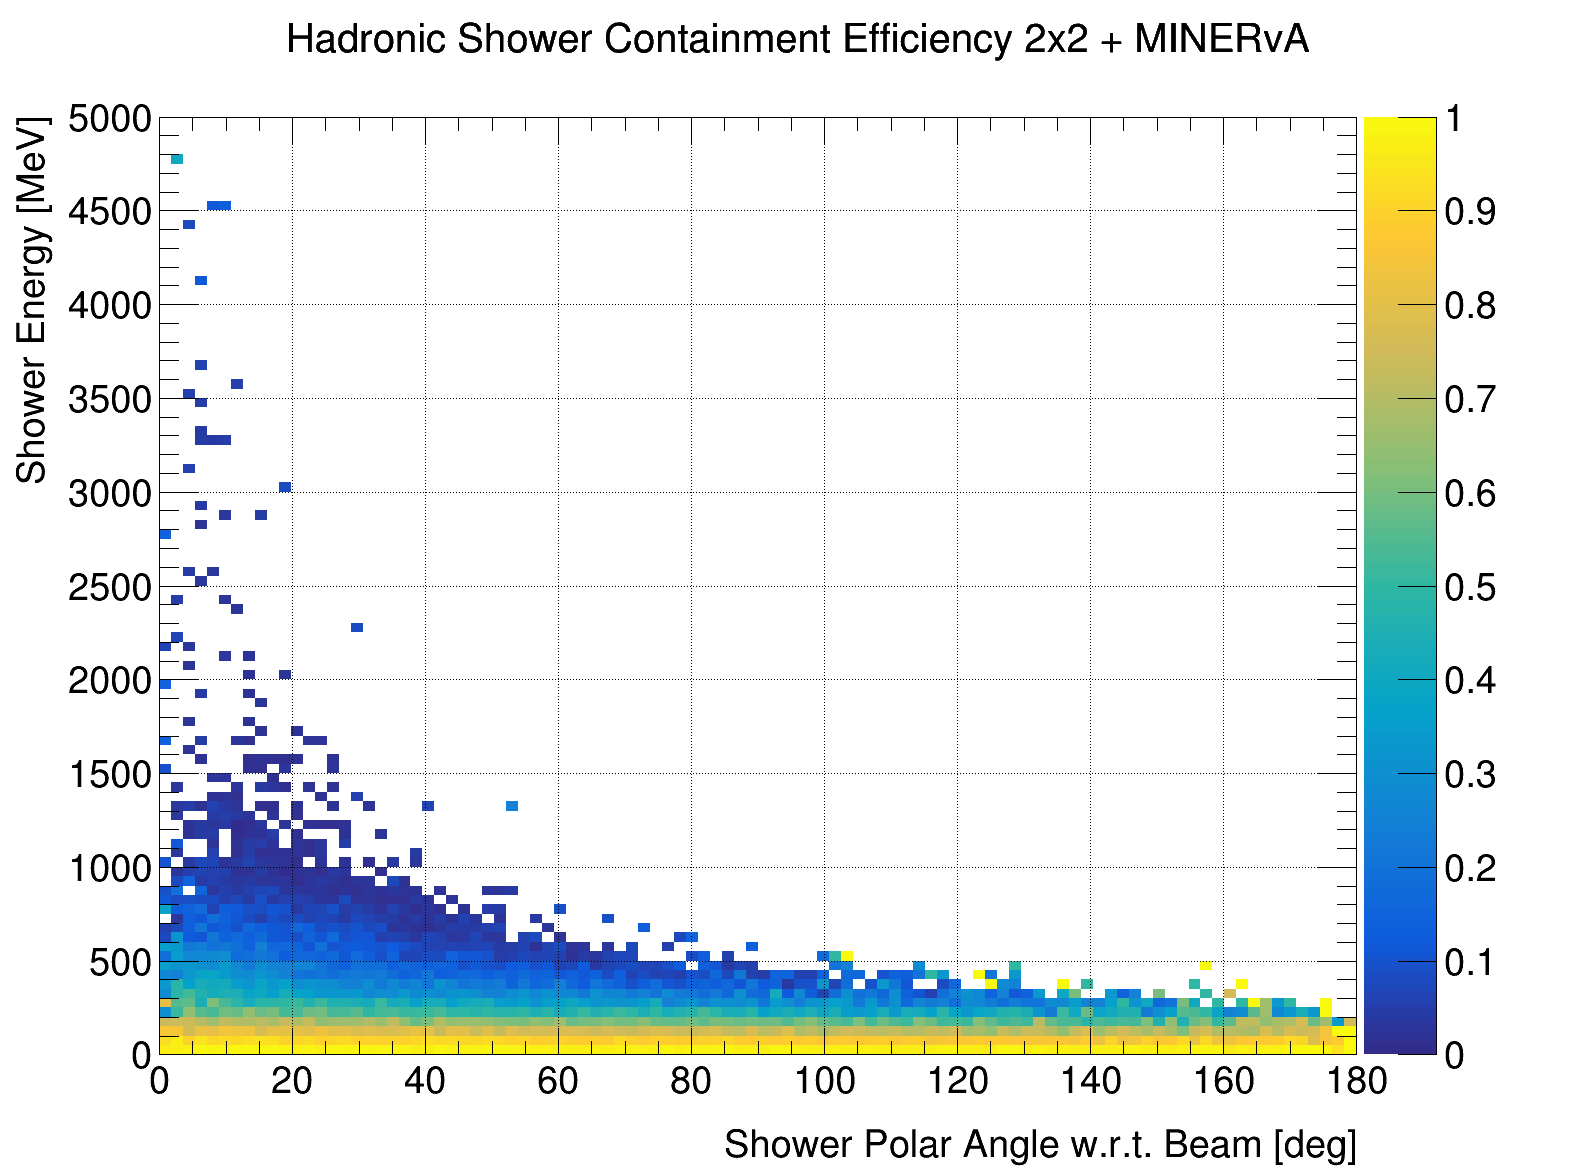
\includegraphics[width=0.45\textwidth]{plots/2x2_minerva_plots/H_cont_eff_2x2_MINERvA.png}}
  \caption{Efficiency for containing hadronic showers, in the 2x2-only, and 2x2+MINERvA, as a function of hadronic shower energy and angle w.r.t the incoming neutrino direction. Containment is defined as $\geq$90\% of the energy being deposited in an active volume of a detector.}
  \label{fig:hadronic_containment}
\end{figure}
In Figure~\ref{fig:hadronic_containment}, the containment of hadron-induced showers is shown as a function of the true energy of the shower, and its angle w.r.t the incoming neutrino beam direction. Showers are defined as being contained when $\geq$90\% of the true energy of the shower is deposited inside the active 2x2 volume, or the MINERvA component if applicable. As expected, including a MINERvA component downstream of the 2x2 module increases the efficiency for angles $\theta \lesssim 30^{\circ}$, which dramatically increases the containment of high energy $E \gtrsim 0.5$ GeV hadronic showers, which tend to be forward-going.

\begin{figure}[htb]
  \centering
  \subfloat[2x2-only]    {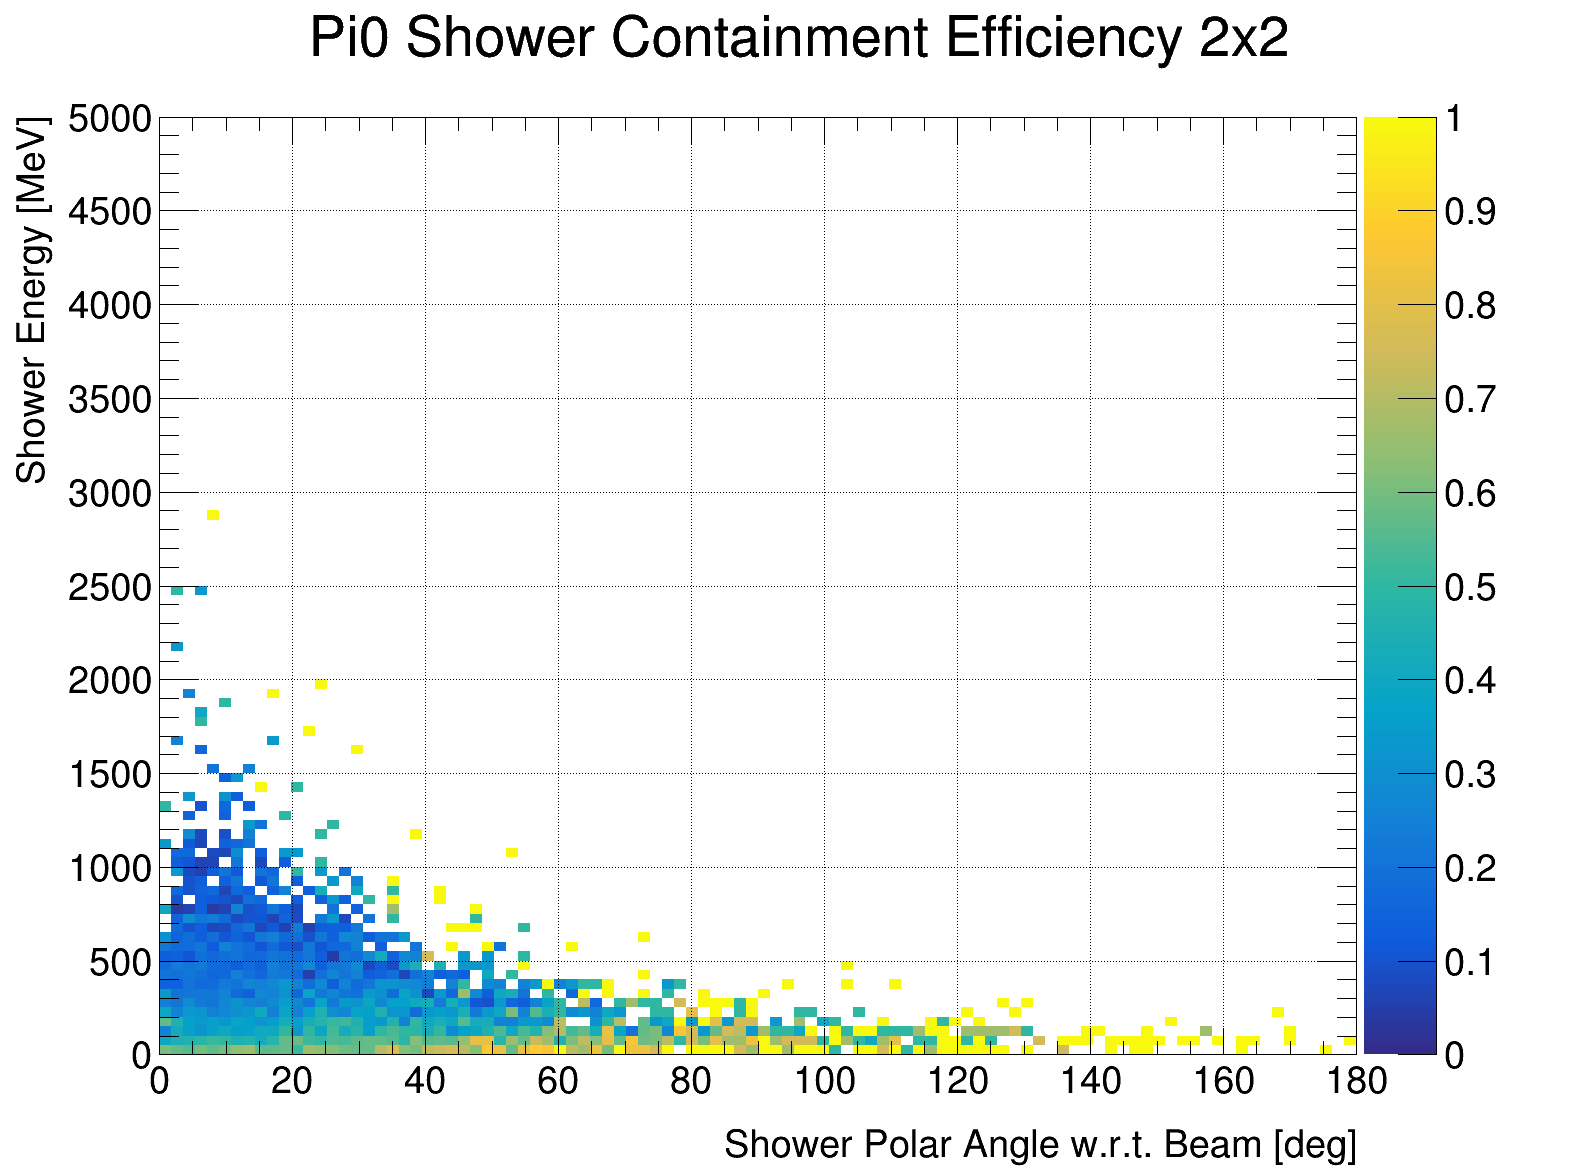
\includegraphics[width=0.45\textwidth]{plots/2x2_minerva_plots/Pi0_cont_eff_2x2.png}}
  \subfloat[2x2+MINERvA] {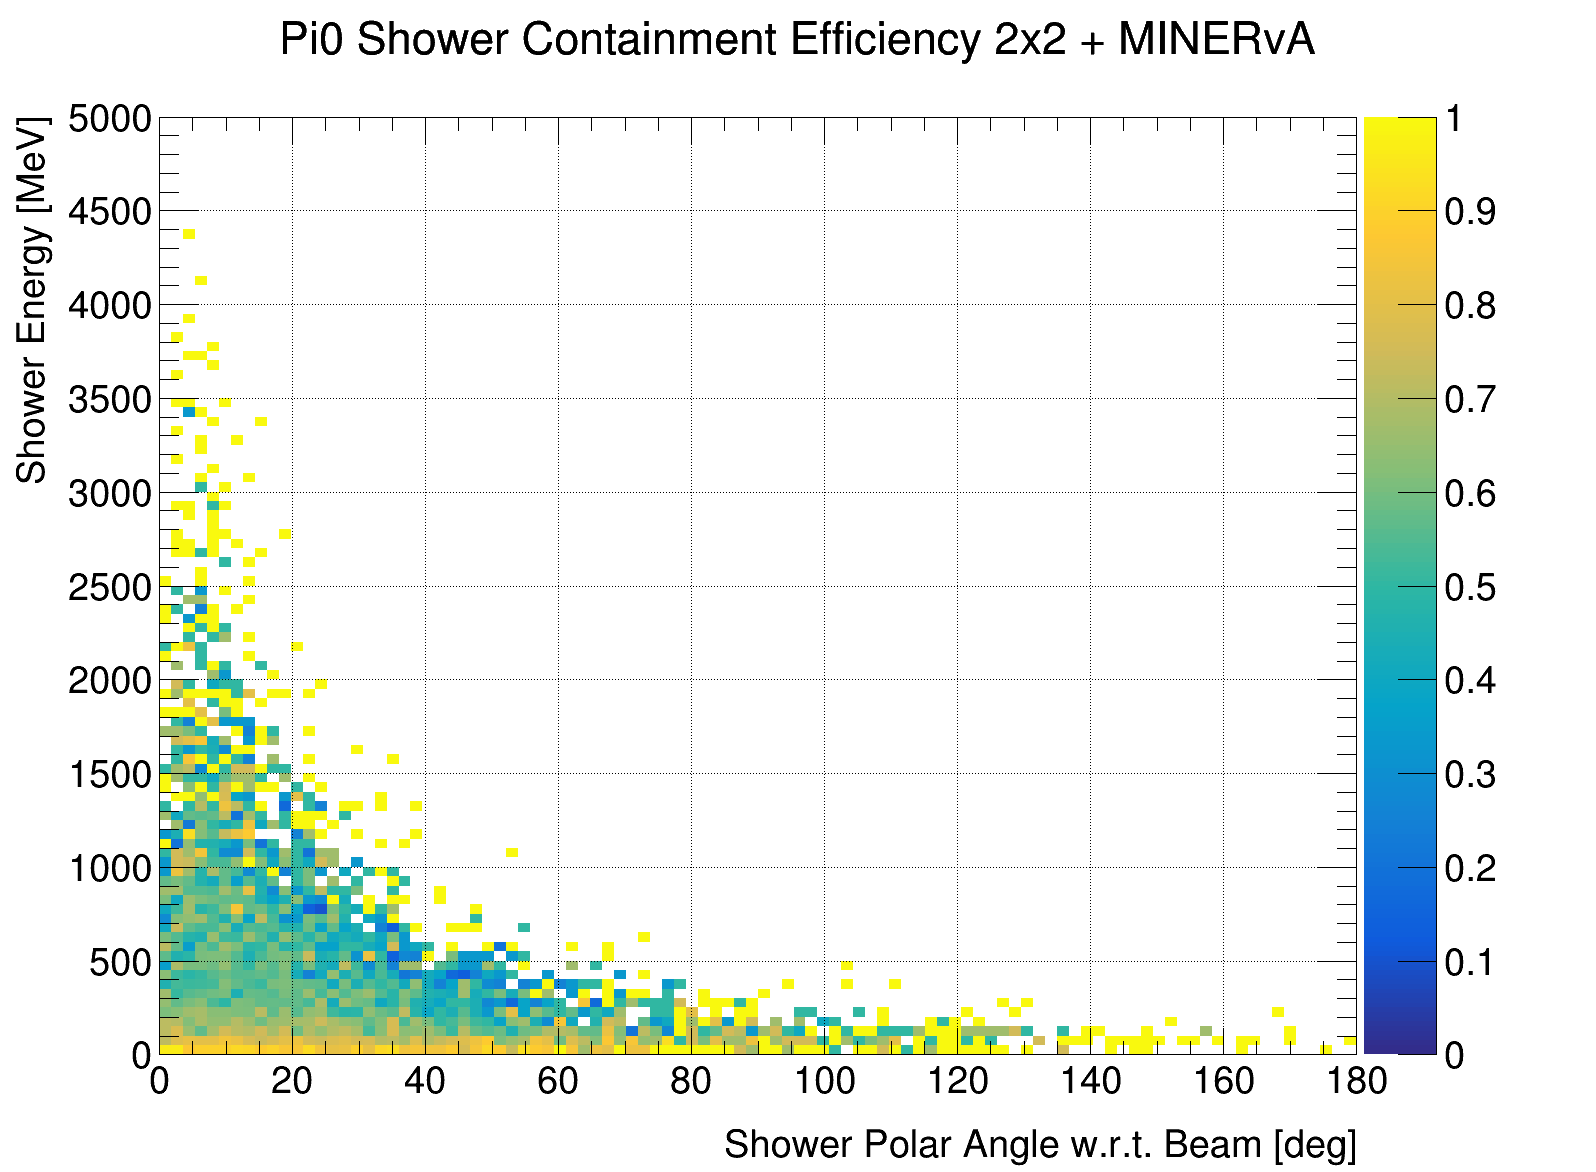
\includegraphics[width=0.45\textwidth]{plots/2x2_minerva_plots/Pi0_cont_eff_2x2_MINERvA.png}}
  \caption{Efficiency for containing both photon-induced showers from $\pi^{0}$ decays, in the 2x2-only, and 2x2+MINERvA, as a function of the $\pi^{0}$ kinetic energy and angle w.r.t the incoming neutrino direction. Containment is defined as $\geq$90\% of the energy being deposited in an active volume of a detector.}
  \label{fig:pi0_containment}
\end{figure}
As discussed previously in this note, as the 2x2 module will not be placed in a test beam prior to installation in the NuMI beam at Fermilab, measurements in which the energy scale of the 2x2 can be calibration will be vital to assess the quality of energy reconstruction in the detector. The containment of both photons from a $\pi^{0}$ decay provides an appropriate in situ measurment of the energy reconstruction capabilities. In Figure~\ref{fig:pi0_containment}, the efficiency to contain 90\% of the energy from both photon-induced showers from a $\pi^{0}$ decay within the active volume of the 2x2, or the MINERvA component if relevant, is shown as a function of the $\pi^{0}$ kinetic energy and angle w.r.t the incoming neutrino beam. There is a significant increase in efficiency for all kinetic energies above a few hundred MeV, particularly for high energy ($E_{\pi^{0}} \gtrsim 1$ GeV) pions, which are produced in the forward direction. Although the dead space between the ArconCube 2x2 active volume and the MINERvA component complicates this picture somewhat, it is clear that including a large portion of MINERvA would give much greater statistics for this benchmark test of the ArgonCube detector performance.

\subsubsection{Neutron tagging studies}

\begin{figure}[htb]
  \centering
  \subfloat[2x2]    {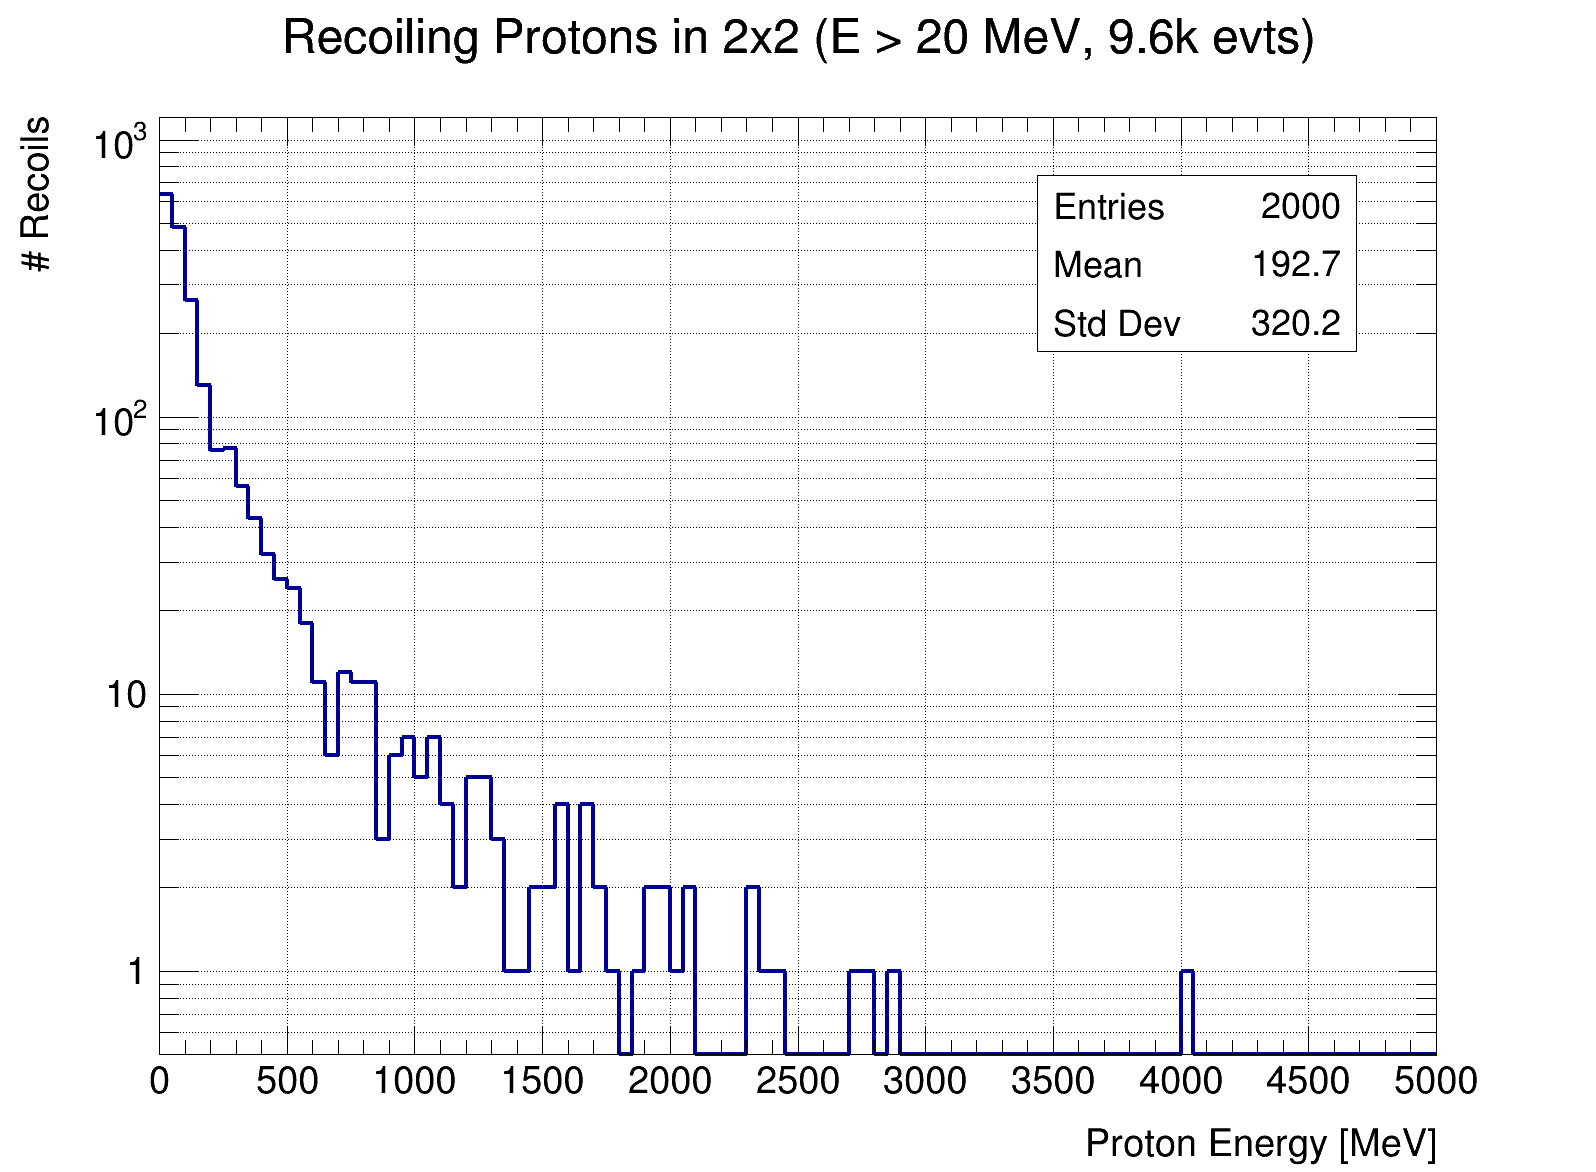
\includegraphics[width=0.45\textwidth]{plots/2x2_minerva_plots/recoils_vs_E_proton_2x2.png}}
  \subfloat[MINERvA] {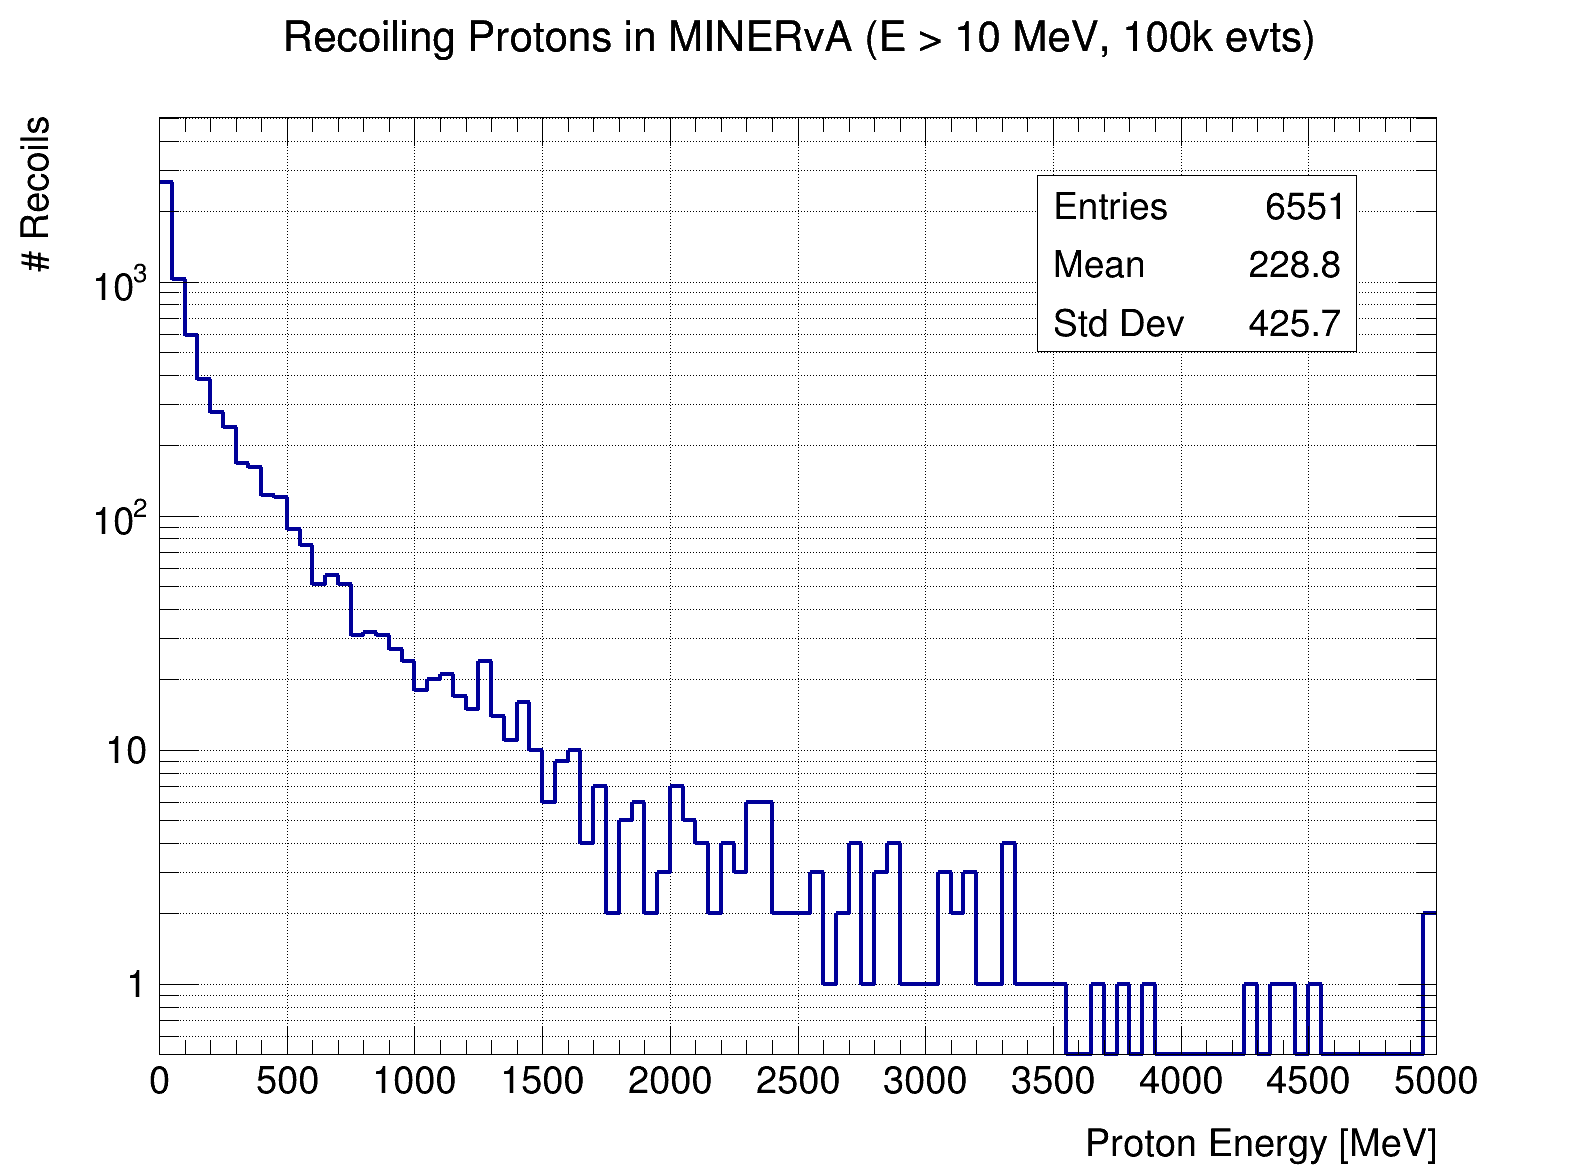
\includegraphics[width=0.45\textwidth]{plots/2x2_minerva_plots/recoils_vs_E_proton_MINERvA.png}}
  \caption{Number of neutron-induced proton recoils as a function of proton energy, which originate from an interaction vertex in the 2x2 active volume, seen in both the 2x2 ative volume, and the downstream MINERvA detector.}
  \label{fig:neutron_tag_minerva}
\end{figure}

As discussed in Section~\ref{sec:2x2_neutron}, one key detector physics goal with ProtoDUNE-ND is to determine whether neutron-induced proton recoils can be identified in a LAr TPC, specifically in ArgonCube. The ability to identify and measure neutrons produced in neutrino interactions is of great interest to DUNE.  At the far detector recoil protons can be identified and easily associated to the neutrino interaction.  However, at the near detector, confusion due to multiple neutrino interactions in the same beam spill poses a unique challenge.  Because neutrons can travel $\mathcal{O}\left(1\right)\,\mathrm{m}$ in LAr without interacting, and proton recoils from fast neutrons typically deposit energy on a single pixel and thus contain no directionality, event association is not possible without matching the charge deposit to an ArCLight optical flash with fast timing resolution.
 
Additionally, it may be possible to measure the neutron energy from time of flight in the DUNE ND using the ECAL with very fast, sub-nanosecond timing resolution. This will require matching muon tracks from either the LAr or HPGAR TPCs to hits in the ECAL to reconstruct the neutrino interaction vertex time with high precision, and also identify and timestamp a subsequent neutron interaction in the scintillator tiles of the ECAL. This would give the DUNE ND unprecedented ability to make measurements of the neutron energy spectrum in neutrino-argon interactions. This technique has not been tested in a high rate environment. Because the neutrons may propagate for $\mathcal{O}\left(10\right)\,\mathrm{ns}$, even a very fast detector may suffer from confusion due to pile-up.

MINERvA can detect neutron-induced proton recoils down to energies of a few MeV, and measure the 3D position of a recoil with a threshold of 20~MeV.  MINERvA has an established neutron reconstruction and a relatively well-understood detector response.  As shown in Fig. 24, it will be possible to reconstruct neutrons originating in the LAr of the ArgonCube 2x2 Demonstrator by their interactions in MINERvA. The ability to match both muons and neutrons originating in LAr to a fast-timing scintillator detector would be a direct test of the feasibility of this technique in DUNE ND. This has profound impact on the design of the ECAL, which would need to be optimized for both EM and neutron reconstruction if this technique is demonstrated to be viable. 
 
 
\FloatBarrier
\subsection{Magnetized low-density tracking detector}
The DUNE ND will employ a downstream tracking detector to measure forward, high-energy muons, and will be sufficiently wide as to contain muons at high angles.  However, for wide-angle muons, tracks will only be contained when the vertex is far from the edges, and will often exit the TPC and not be reconstructed.  This sample could be recovered if the muon momentum can be measured reliably from multiple coulomb scattering (MCS). The far detector will also use MCS for muons which exit the detector.

Such measurements have been carried out in a LAr TPC by MicroBooNE~\cite{Abratenko:2017nki}, although the momentum range is somewhat limited as the only validation sample available is composed of muons which stop in the detector, for which a momentum by range measurement can be made. However, such measurements may be more challenging in a modular TPC such as ArgonCube, where tracks are necessarily broken into segments which are read out separately, and then combined in downstream software.

Although there are only four modules in the ArgonCube 2x2 Demonstrator, each is split into two TPCs, so tracks which exit the downstream face of the 2x2 module may be sampled by up to four independent charge readout planes. With a downstream detector capable of making a precise muon momentum measurement, it would be possible to demonstrate that multiple coulomb scattering will be a viable technique for making momentum measurements in the full ArgonCube deployment in the DUNE ND. Given the hard muon momentum spectrum expected in the NuMI on-axis beam (shown in Figure~\ref{fig:momenta}), it would be hard to make a reliable momentum measurement with a small demonstrator tracker module, or indeed with the MINERvA components proposed in Section~\ref{sec:minerva}, as few would be contained. Such measurements could be made, in the MINOS-ND, which is capable of making momentum measurements for all relevant muon momenta by curvature, or by range.


\section{Cosmic Ray Tagger}

In practice, these panels could be used to better identify a sample of fully contained neutrino events for the studies outlined in Sections~\ref{sec:minerva-acceptance}. Additionally, these cosmic ray tagging modules could then be used to validate space charge build-up and electric field uniformity studies outlined in Section~\ref{sec:efield}, and the cosmic suppression studies described in Section~\ref{sec:cosmic-suppression}, for which an additional scintillator panel would be required.

\subsection{Space charge and electric field uniformity}
\label{sec:efield}
A concern for LAr detectors in a high intensity beam is the build up of space charge --- long-lived argon ions which drift slowly towards the cathode --- and possible affects on the uniformity of the electric field which may accumulate over time. In currently operating and near-future LAr detectors~\cite{Ereditato:2014lra, Antonello:2015lea}, both cosmic tracks and UV lasers are used to calibrate for distortions in the electric field. Both the UV laser track and high energy cosmic muons are expected to leave straight tracks in the detector. If the drift field is not uniform across the detector, ionization electrons produced along the length of this track will not drift at the same speed, or with a constant direction, and will result in a distorted track at the readout plane. By comparing the reconstructed and expected track, a map of the electric field distortion can be built up for calibration purposes.

Assuming that the ArgonCube 2x2 Demonstrator is equipped with scintillator panels to tag cosmic tracks using a timing coincidence between two sides of the detector, and reasonable spatial resolution on those scintillator paddles, electric field distortions could be measured in the 2x2 Demonstrator module. By looking at beam-on, and beam-off data, it would be possible to look at the possible affect of space charge build-up over time due to the high event rate in the NuMI beam. If significant space charge build-up were observed, this would inform the future ArgonCube design for the DUNE ND, as a higher drift field strength would be required.

Additionally, although the electric-field uniformity of the resistive field shell will be checked in a small scale LAr TPC at Bern, a check of the electric-field uniformity and stability over time for full-size ArgonCube modules would be a valuable final validation of the design.

\subsection{Cosmic and Rock Muon suppression}
\label{sec:cosmic-suppression}

The DUNE ND is located underground with a \SI{50}{\metre} overburden, that reduces the cosmic flux by orders of magnitude compared to surface detectors. The cosmic rate in MINERvA (currently in the MINOS ND hall where ProtoDUNE-ND will be sited) is \SI{18}{\hertz}, for $\sim$\SI{6}{\metre\squared}. For the ArgonCube 2x2, in the $\sim$\SI{150}{\micro\second} readout window, assuming $\sim$\SI{2}{\metre\squared}, the rate of cosmics muons is 0.001 per readout window. Reading out around spills only, will result in a coincident cosmic muon once every 20 minutes.
In DUNE ND we expect $\sim$10 rock muons per spill, which will be on average $\sim$\SI{1}{\micro\second} apart in time. They are unlikely to overlap any neutrino activity in 3D, but the fast timing will provide an additional handle.
A key design choice for the DUNE ND is whether or not a muon tagging system is required --- for example, a series of scintillator planes surrounding the LAr TPC, as for SBND and MicroBooNE~\cite{CRT}. The proposed ProtoDUNE-ND test experiment can help inform this design choice, assuming that the ArgonCube 2x2 Demonstrator module is equipped with scintillator paddles.

By using the scintillator paddles to tag cosmic or rock events using a timing coincidence, methods for rejecting them can be validated independently. For example, we expect that the good timing resolution and light localization from ArcLight will allow cosmics out of the beam window to be rejected with a high efficiency. Additionally, if a cosmic muon traverses a pixel plane, or an ArcLight plane, we would expect to see a large charge deposition or a large number of photoelectrons measured, which could be an additional way to reject cosmic muons. Both of these methods can be validated with ProtoDUNE-ND.

\section{Outlook and timeline}
\label{sec:outlook}
To provide some context for the aggressive schedule of the ArgonCube 2x2 Demonstrator and ProtoDUNE-ND: the Conceptual Design Report for the DUNE ND will be submitted in April of 2019, with the Technical Design Report to be submitted in April of the following year~\cite{dune_dates}, with installation due to begin in 2025. 

The 2x2 construction and commissioning will take place in Bern, before the detector is moved to Fermilab. To date, the various technologies have been demonstrated in small test stands, the next step is to test the module construction techniques. Once these tests are complete, the technologies can be scaled to populate a 2x2 module. The following is a very simplified timeline indicating the major milestones and contributing institutes:      

\begin{itemize}
\item {\bf December 2018:}
\begin{itemize}
\item Bern: Complete cryostat instrumentation and infrastructure: for cryogenic control systems and slow control monitoring. 
\item LBNL: LArPix V2 design to vendor. Packaging test with LArPix V1.
\end{itemize}
\item {\bf January 2019:} 
\begin{itemize}
	\item Bern: Test of first module, demonstrate purity can be maintained, confirm material choices, optimize cooling control and slow monitoring system.   
	\item LBNL: LArPix V2 review meeting. LArPix V2 Production.
	\item SLAC: Review resistive-shell TPC construction techniques. Review HV supply and distribution options.   
	\item FNAL: Control system development (PLC). Determine cryogenic infrastructure requirements at FNAL (ODH), and cost 
	estimate.  
\end{itemize}
\item {\bf February 2019:} FNAL: Cryogenic review meeting.  
\item {\bf March 2019:} Bern: Deploy FNAL PLC. Collaboration meeting, finalize module design and outline construction workload across collaboration.    
\item {\bf April 2019:} 
\begin{itemize}
	\item Rochester: Review rock-muon tagger. Finalize design concept of beam trigger and high level DAQ (event builder). 
	\item FNAL: Review MINOS ND hall installation concept.  
\end{itemize}
\item {\bf June 2019:} Collaboration: Preliminary MINOS ND hall installation plan.
\item {\bf July 2019:} 
\begin{itemize}
	\item LBNL: Testing of LArPix V2 on pixel PCB.   
	\item SLAC: Finalize TPC construction method.
	%\item Rochester: Review design options for movable 2x2 platform and sump.  
\end{itemize}
\item {\bf September 2019:} Collaboration work at Bern: Module component delivery to Bern, QA/QC.
\item {\bf October/November 2019:} Collaboration work at Bern: Module construction begins.
\item {\bf December 2019:} 
\begin{itemize}
	\item Collaboration work at Bern: Cosmic run  2x2, DAQ tests and develop simple reconstruction tools.   
	\item FNAL: Review installation design.  
\end{itemize}
\item {\bf January 2020:}
\begin{itemize}
	\item Bern: Shipping to FNAL.
	\item Rochester at FNAL: Trigger/DAQ electronics installation and commissioning. 
\end{itemize}
\item {\bf February 2020:} Collaboration work at FNAL: 2x2 assembly and installation.
\item {\bf May 2020:} Collaboration work at FNAL: 2x2 commissioning.    
\item {\bf October 2020:} Collaboration work at FNAL: Beginning of beam data. Calibrations and data analysis.

\end{itemize}

\section{Conclusions}
\label{sec:conclusions}

In this work, we have outlined the detector physics potential of the ProtoDUNE-ND testbench experiment in the MINOS-ND hall at Fermilab, which is intended to be a ``neutrino engineering'' test. At the heart of ProtoDUNE-ND sits the ArgonCube 2x2 Demonstrator module, which is currently being commissioned, and will be moved to Fermilab by early 2020. The set-up of ProtoDUNE-ND is intended to be flexible, to allow for new modules testing different aspects of the future DUNE-ND design to be installed at different times. This is facilitated by the moveable cryogenic support systems which need to be tested for the DUNE-PRISM baseline design concept, and which will allow the ArgonCube 2x2 to be moved, and the ProtoDUNE-ND arrangement to be reconfigured as a result. The detector physics studies outlined in this document will provide vital inputs to the full-scale DUNE-ND design, and provide a much-needed intermediate scale test, scaling up the small R\&D tests which have already been carried out, and allowing for long-term stability tests to be carried out.

In this document, we have also outlined the detector physics case for incorporating elements of the soon to be decommissioned MINERvA detector into the ProtoDUNE-ND setup, provided all infrastructure and resource availability needs can be met. All DUNE-ND designs considered in Ref.~\cite{dune_ndcsg} include some fast scintillator detector, but no prototype is foreseen at this time for ProtoDUNE-ND. MINERvA components would fill that gap, and provide an essential test of combined reconstruction across different detectors will very different readout technology and times. Additionally, we briefly discussed the possibility to include the MINOS-ND into ProtoDUNE-ND, which is due to be decommissioned along with the MINERA experiment in mid-2019. In combination, using elements of MINERvA and MINOS-ND in ProtoDUNE-ND would allow us to contain all particles in a large fraction of events, and provide a realistic test of the energy recontruction capabilities of the final DUNE-ND. This would be invaluable for DUNE-ND design studies, and would enhance the impact of the ProtoDUNE-ND test.


\printbibliography

%\begin{acknowledgments}
%Thanks for all the \$\$\$
%\end{acknowledgments}


%\bibliography{bibliography.bib}% Produces the bibliography via BibTeX.

%\appendix
%\input{an_appendix}

\end{document}
